\documentclass[12pt]{article}
\usepackage[english]{babel}
\usepackage[utf8x]{inputenc}
\usepackage{amsmath}
\usepackage{graphicx}
\usepackage[colorinlistoftodos]{todonotes}
\usepackage{array}
\usepackage{multirow}
\usepackage{tabularx}
\usepackage{textcomp}
\usepackage{gensymb}
\usepackage{listings}
\usepackage{courier}
\usepackage{fancyhdr}
\usepackage{nameref}
\usepackage{pdflscape}
\usepackage{rotating}
\usepackage{csvsimple}
\usepackage{longtable}
\usepackage{pdfpages}

\makeatletter
\newcommand*{\currentname}{\@currentlabelname}
\makeatother

\newcommand*{\frontmatter}{\pagenumbering{roman}}
\newcommand*{\mainmatter}{
    \pagenumbering{arabic}
    \pagestyle{fancy}
    \fancyhf{}
    \lhead{DynaSaRR}
    \rhead{\currentname}
    \renewcommand{\footrulewidth}{0.5pt}
    \rfoot{Page \thepage}
}
\newcommand*{\backmatter}{
    \pagenumbering{Roman}
    \thispagestyle{plain}
}

\fancypagestyle{mylandscape}{%
  \fancyhf{}% Clear header/footer
  \fancyfoot{% Footer
    \makebox[\textwidth][r]{% Right
      \rlap{\hspace{\footskip}% Push out of margin by \footskip
        \smash{% Remove vertical height
          \raisebox{\dimexpr.5\baselineskip+\footskip+.5\textheight}{% Raise vertically
            \rotatebox{90}{\thepage}}}}}}% Rotate counter-clockwise
  \renewcommand{\headrulewidth}{0pt}% No header rule
  \renewcommand{\footrulewidth}{0pt}% No footer rule
}
\graphicspath{ {Images/} }

 %%%%%%%%%%%%%%%%%%%%%%%%%%%%%%%%%%%%%%%%%%%%%%%%%%%%%%%%%%%%%%%%%%%%%%%%%%%%%%%% 
%%% ~ Arduino Language - Arduino IDE Colors ~                                  %%%
%%%                                                                            %%%
%%% Kyle Rocha-Brownell | 10/2/2017 | No Licence                               %%%
%%% -------------------------------------------------------------------------- %%%
%%%                                                                            %%%
%%% Place this file in your working directory (next to the latex file you're   %%%
%%% working on).  To add it to your project, place:                            %%%
%%%     %%%%%%%%%%%%%%%%%%%%%%%%%%%%%%%%%%%%%%%%%%%%%%%%%%%%%%%%%%%%%%%%%%%%%%%%%%%%%%%% 
%%% ~ Arduino Language - Arduino IDE Colors ~                                  %%%
%%%                                                                            %%%
%%% Kyle Rocha-Brownell | 10/2/2017 | No Licence                               %%%
%%% -------------------------------------------------------------------------- %%%
%%%                                                                            %%%
%%% Place this file in your working directory (next to the latex file you're   %%%
%%% working on).  To add it to your project, place:                            %%%
%%%     %%%%%%%%%%%%%%%%%%%%%%%%%%%%%%%%%%%%%%%%%%%%%%%%%%%%%%%%%%%%%%%%%%%%%%%%%%%%%%%% 
%%% ~ Arduino Language - Arduino IDE Colors ~                                  %%%
%%%                                                                            %%%
%%% Kyle Rocha-Brownell | 10/2/2017 | No Licence                               %%%
%%% -------------------------------------------------------------------------- %%%
%%%                                                                            %%%
%%% Place this file in your working directory (next to the latex file you're   %%%
%%% working on).  To add it to your project, place:                            %%%
%%%    \input{arduinoLanguage.tex}                                             %%%
%%% somewhere before \begin{document} in your latex file.                      %%%
%%%                                                                            %%%
%%% In your document, place your arduino code between:                         %%%
%%%   \begin{lstlisting}[language=Arduino]                                     %%%
%%% and:                                                                       %%%
%%%   \end{lstlisting}                                                         %%%
%%%                                                                            %%%
%%% Or create your own style to add non-built-in functions and variables.      %%%
%%%                                                                            %%%
 %%%%%%%%%%%%%%%%%%%%%%%%%%%%%%%%%%%%%%%%%%%%%%%%%%%%%%%%%%%%%%%%%%%%%%%%%%%%%%%% 

\usepackage{color}
\usepackage{listings}    
\usepackage{courier}

%%% Define Custom IDE Colors %%%
\definecolor{arduinoGreen}    {rgb} {0.17, 0.43, 0.01}
\definecolor{arduinoGrey}     {rgb} {0.47, 0.47, 0.33}
\definecolor{arduinoOrange}   {rgb} {0.8 , 0.4 , 0   }
\definecolor{arduinoBlue}     {rgb} {0.01, 0.61, 0.98}
\definecolor{arduinoDarkBlue} {rgb} {0.0 , 0.2 , 0.5 }

%%% Define Arduino Language %%%
\lstdefinelanguage{Arduino}{
  language=C++, % begin with default C++ settings 
%
%
  %%% Keyword Color Group 1 %%%  (called KEYWORD3 by arduino)
  keywordstyle=\color{arduinoGreen},   
  deletekeywords={  % remove all arduino keywords that might be in c++
                break, case, override, final, continue, default, do, else, for, 
                if, return, goto, switch, throw, try, while, setup, loop, export, 
                not, or, and, xor, include, define, elif, else, error, if, ifdef, 
                ifndef, pragma, warning,
                HIGH, LOW, INPUT, INPUT_PULLUP, OUTPUT, DEC, BIN, HEX, OCT, PI, 
                HALF_PI, TWO_PI, LSBFIRST, MSBFIRST, CHANGE, FALLING, RISING, 
                DEFAULT, EXTERNAL, INTERNAL, INTERNAL1V1, INTERNAL2V56, LED_BUILTIN, 
                LED_BUILTIN_RX, LED_BUILTIN_TX, DIGITAL_MESSAGE, FIRMATA_STRING, 
                ANALOG_MESSAGE, REPORT_DIGITAL, REPORT_ANALOG, SET_PIN_MODE, 
                SYSTEM_RESET, SYSEX_START, auto, int8_t, int16_t, int32_t, int64_t, 
                uint8_t, uint16_t, uint32_t, uint64_t, char16_t, char32_t, operator, 
                enum, delete, bool, boolean, byte, char, const, false, float, double, 
                null, NULL, int, long, new, private, protected, public, short, 
                signed, static, volatile, String, void, true, unsigned, word, array, 
                sizeof, dynamic_cast, typedef, const_cast, struct, static_cast, union, 
                friend, extern, class, reinterpret_cast, register, explicit, inline, 
                _Bool, complex, _Complex, _Imaginary, atomic_bool, atomic_char, 
                atomic_schar, atomic_uchar, atomic_short, atomic_ushort, atomic_int, 
                atomic_uint, atomic_long, atomic_ulong, atomic_llong, atomic_ullong, 
                virtual, PROGMEM,
                Serial, Serial1, Serial2, Serial3, SerialUSB, Keyboard, Mouse,
                abs, acos, asin, atan, atan2, ceil, constrain, cos, degrees, exp, 
                floor, log, map, max, min, radians, random, randomSeed, round, sin, 
                sq, sqrt, tan, pow, bitRead, bitWrite, bitSet, bitClear, bit, 
                highByte, lowByte, analogReference, analogRead, 
                analogReadResolution, analogWrite, analogWriteResolution, 
                attachInterrupt, detachInterrupt, digitalPinToInterrupt, delay, 
                delayMicroseconds, digitalWrite, digitalRead, interrupts, millis, 
                micros, noInterrupts, noTone, pinMode, pulseIn, pulseInLong, shiftIn, 
                shiftOut, tone, yield, Stream, begin, end, peek, read, print, 
                println, available, availableForWrite, flush, setTimeout, find, 
                findUntil, parseInt, parseFloat, readBytes, readBytesUntil, readString, 
                readStringUntil, trim, toUpperCase, toLowerCase, charAt, compareTo, 
                concat, endsWith, startsWith, equals, equalsIgnoreCase, getBytes, 
                indexOf, lastIndexOf, length, replace, setCharAt, substring, 
                toCharArray, toInt, press, release, releaseAll, accept, click, move, 
                isPressed, isAlphaNumeric, isAlpha, isAscii, isWhitespace, isControl, 
                isDigit, isGraph, isLowerCase, isPrintable, isPunct, isSpace, 
                isUpperCase, isHexadecimalDigit, 
                }, 
  morekeywords={   % add arduino structures to group 1
                break, case, override, final, continue, default, do, else, for, 
                if, return, goto, switch, throw, try, while, setup, loop, export, 
                not, or, and, xor, include, define, elif, else, error, if, ifdef, 
                ifndef, pragma, warning,
                }, 
% 
%
  %%% Keyword Color Group 2 %%%  (called LITERAL1 by arduino)
  keywordstyle=[2]\color{arduinoBlue},   
  keywords=[2]{   % add variables and dataTypes as 2nd group  
                HIGH, LOW, INPUT, INPUT_PULLUP, OUTPUT, DEC, BIN, HEX, OCT, PI, 
                HALF_PI, TWO_PI, LSBFIRST, MSBFIRST, CHANGE, FALLING, RISING, 
                DEFAULT, EXTERNAL, INTERNAL, INTERNAL1V1, INTERNAL2V56, LED_BUILTIN, 
                LED_BUILTIN_RX, LED_BUILTIN_TX, DIGITAL_MESSAGE, FIRMATA_STRING, 
                ANALOG_MESSAGE, REPORT_DIGITAL, REPORT_ANALOG, SET_PIN_MODE, 
                SYSTEM_RESET, SYSEX_START, auto, int8_t, int16_t, int32_t, int64_t, 
                uint8_t, uint16_t, uint32_t, uint64_t, char16_t, char32_t, operator, 
                enum, delete, bool, boolean, byte, char, const, false, float, double, 
                null, NULL, int, long, new, private, protected, public, short, 
                signed, static, volatile, String, void, true, unsigned, word, array, 
                sizeof, dynamic_cast, typedef, const_cast, struct, static_cast, union, 
                friend, extern, class, reinterpret_cast, register, explicit, inline, 
                _Bool, complex, _Complex, _Imaginary, atomic_bool, atomic_char, 
                atomic_schar, atomic_uchar, atomic_short, atomic_ushort, atomic_int, 
                atomic_uint, atomic_long, atomic_ulong, atomic_llong, atomic_ullong, 
                virtual, PROGMEM,
                },  
% 
%
  %%% Keyword Color Group 3 %%%  (called KEYWORD1 by arduino)
  keywordstyle=[3]\bfseries\color{arduinoOrange},
  keywords=[3]{  % add built-in functions as a 3rd group
                Serial, Serial1, Serial2, Serial3, SerialUSB, Keyboard, Mouse,
                },      
%
%
  %%% Keyword Color Group 4 %%%  (called KEYWORD2 by arduino)
  keywordstyle=[4]\color{arduinoOrange},
  keywords=[4]{  % add more built-in functions as a 4th group
                abs, acos, asin, atan, atan2, ceil, constrain, cos, degrees, exp, 
                floor, log, map, max, min, radians, random, randomSeed, round, sin, 
                sq, sqrt, tan, pow, bitRead, bitWrite, bitSet, bitClear, bit, 
                highByte, lowByte, analogReference, analogRead, 
                analogReadResolution, analogWrite, analogWriteResolution, 
                attachInterrupt, detachInterrupt, digitalPinToInterrupt, delay, 
                delayMicroseconds, digitalWrite, digitalRead, interrupts, millis, 
                micros, noInterrupts, noTone, pinMode, pulseIn, pulseInLong, shiftIn, 
                shiftOut, tone, yield, Stream, begin, end, peek, read, print, 
                println, available, availableForWrite, flush, setTimeout, find, 
                findUntil, parseInt, parseFloat, readBytes, readBytesUntil, readString, 
                readStringUntil, trim, toUpperCase, toLowerCase, charAt, compareTo, 
                concat, endsWith, startsWith, equals, equalsIgnoreCase, getBytes, 
                indexOf, lastIndexOf, length, replace, setCharAt, substring, 
                toCharArray, toInt, press, release, releaseAll, accept, click, move, 
                isPressed, isAlphaNumeric, isAlpha, isAscii, isWhitespace, isControl, 
                isDigit, isGraph, isLowerCase, isPrintable, isPunct, isSpace, 
                isUpperCase, isHexadecimalDigit, 
                },      
%
%
  %%% Set Other Colors %%%
  stringstyle=\color{arduinoDarkBlue},    
  commentstyle=\color{arduinoGrey},    
%          
%   
  %%%% Line Numbering %%%%
   numbers=left,                    
  numbersep=5pt,                   
  numberstyle=\color{arduinoGrey},    
  %stepnumber=2,                      % show every 2 line numbers
%
%
  %%%% Code Box Style %%%%
  breaklines=true,                    % wordwrapping
  tabsize=2,         
  basicstyle=\ttfamily  
}                                             %%%
%%% somewhere before \begin{document} in your latex file.                      %%%
%%%                                                                            %%%
%%% In your document, place your arduino code between:                         %%%
%%%   \begin{lstlisting}[language=Arduino]                                     %%%
%%% and:                                                                       %%%
%%%   \end{lstlisting}                                                         %%%
%%%                                                                            %%%
%%% Or create your own style to add non-built-in functions and variables.      %%%
%%%                                                                            %%%
 %%%%%%%%%%%%%%%%%%%%%%%%%%%%%%%%%%%%%%%%%%%%%%%%%%%%%%%%%%%%%%%%%%%%%%%%%%%%%%%% 

\usepackage{color}
\usepackage{listings}    
\usepackage{courier}

%%% Define Custom IDE Colors %%%
\definecolor{arduinoGreen}    {rgb} {0.17, 0.43, 0.01}
\definecolor{arduinoGrey}     {rgb} {0.47, 0.47, 0.33}
\definecolor{arduinoOrange}   {rgb} {0.8 , 0.4 , 0   }
\definecolor{arduinoBlue}     {rgb} {0.01, 0.61, 0.98}
\definecolor{arduinoDarkBlue} {rgb} {0.0 , 0.2 , 0.5 }

%%% Define Arduino Language %%%
\lstdefinelanguage{Arduino}{
  language=C++, % begin with default C++ settings 
%
%
  %%% Keyword Color Group 1 %%%  (called KEYWORD3 by arduino)
  keywordstyle=\color{arduinoGreen},   
  deletekeywords={  % remove all arduino keywords that might be in c++
                break, case, override, final, continue, default, do, else, for, 
                if, return, goto, switch, throw, try, while, setup, loop, export, 
                not, or, and, xor, include, define, elif, else, error, if, ifdef, 
                ifndef, pragma, warning,
                HIGH, LOW, INPUT, INPUT_PULLUP, OUTPUT, DEC, BIN, HEX, OCT, PI, 
                HALF_PI, TWO_PI, LSBFIRST, MSBFIRST, CHANGE, FALLING, RISING, 
                DEFAULT, EXTERNAL, INTERNAL, INTERNAL1V1, INTERNAL2V56, LED_BUILTIN, 
                LED_BUILTIN_RX, LED_BUILTIN_TX, DIGITAL_MESSAGE, FIRMATA_STRING, 
                ANALOG_MESSAGE, REPORT_DIGITAL, REPORT_ANALOG, SET_PIN_MODE, 
                SYSTEM_RESET, SYSEX_START, auto, int8_t, int16_t, int32_t, int64_t, 
                uint8_t, uint16_t, uint32_t, uint64_t, char16_t, char32_t, operator, 
                enum, delete, bool, boolean, byte, char, const, false, float, double, 
                null, NULL, int, long, new, private, protected, public, short, 
                signed, static, volatile, String, void, true, unsigned, word, array, 
                sizeof, dynamic_cast, typedef, const_cast, struct, static_cast, union, 
                friend, extern, class, reinterpret_cast, register, explicit, inline, 
                _Bool, complex, _Complex, _Imaginary, atomic_bool, atomic_char, 
                atomic_schar, atomic_uchar, atomic_short, atomic_ushort, atomic_int, 
                atomic_uint, atomic_long, atomic_ulong, atomic_llong, atomic_ullong, 
                virtual, PROGMEM,
                Serial, Serial1, Serial2, Serial3, SerialUSB, Keyboard, Mouse,
                abs, acos, asin, atan, atan2, ceil, constrain, cos, degrees, exp, 
                floor, log, map, max, min, radians, random, randomSeed, round, sin, 
                sq, sqrt, tan, pow, bitRead, bitWrite, bitSet, bitClear, bit, 
                highByte, lowByte, analogReference, analogRead, 
                analogReadResolution, analogWrite, analogWriteResolution, 
                attachInterrupt, detachInterrupt, digitalPinToInterrupt, delay, 
                delayMicroseconds, digitalWrite, digitalRead, interrupts, millis, 
                micros, noInterrupts, noTone, pinMode, pulseIn, pulseInLong, shiftIn, 
                shiftOut, tone, yield, Stream, begin, end, peek, read, print, 
                println, available, availableForWrite, flush, setTimeout, find, 
                findUntil, parseInt, parseFloat, readBytes, readBytesUntil, readString, 
                readStringUntil, trim, toUpperCase, toLowerCase, charAt, compareTo, 
                concat, endsWith, startsWith, equals, equalsIgnoreCase, getBytes, 
                indexOf, lastIndexOf, length, replace, setCharAt, substring, 
                toCharArray, toInt, press, release, releaseAll, accept, click, move, 
                isPressed, isAlphaNumeric, isAlpha, isAscii, isWhitespace, isControl, 
                isDigit, isGraph, isLowerCase, isPrintable, isPunct, isSpace, 
                isUpperCase, isHexadecimalDigit, 
                }, 
  morekeywords={   % add arduino structures to group 1
                break, case, override, final, continue, default, do, else, for, 
                if, return, goto, switch, throw, try, while, setup, loop, export, 
                not, or, and, xor, include, define, elif, else, error, if, ifdef, 
                ifndef, pragma, warning,
                }, 
% 
%
  %%% Keyword Color Group 2 %%%  (called LITERAL1 by arduino)
  keywordstyle=[2]\color{arduinoBlue},   
  keywords=[2]{   % add variables and dataTypes as 2nd group  
                HIGH, LOW, INPUT, INPUT_PULLUP, OUTPUT, DEC, BIN, HEX, OCT, PI, 
                HALF_PI, TWO_PI, LSBFIRST, MSBFIRST, CHANGE, FALLING, RISING, 
                DEFAULT, EXTERNAL, INTERNAL, INTERNAL1V1, INTERNAL2V56, LED_BUILTIN, 
                LED_BUILTIN_RX, LED_BUILTIN_TX, DIGITAL_MESSAGE, FIRMATA_STRING, 
                ANALOG_MESSAGE, REPORT_DIGITAL, REPORT_ANALOG, SET_PIN_MODE, 
                SYSTEM_RESET, SYSEX_START, auto, int8_t, int16_t, int32_t, int64_t, 
                uint8_t, uint16_t, uint32_t, uint64_t, char16_t, char32_t, operator, 
                enum, delete, bool, boolean, byte, char, const, false, float, double, 
                null, NULL, int, long, new, private, protected, public, short, 
                signed, static, volatile, String, void, true, unsigned, word, array, 
                sizeof, dynamic_cast, typedef, const_cast, struct, static_cast, union, 
                friend, extern, class, reinterpret_cast, register, explicit, inline, 
                _Bool, complex, _Complex, _Imaginary, atomic_bool, atomic_char, 
                atomic_schar, atomic_uchar, atomic_short, atomic_ushort, atomic_int, 
                atomic_uint, atomic_long, atomic_ulong, atomic_llong, atomic_ullong, 
                virtual, PROGMEM,
                },  
% 
%
  %%% Keyword Color Group 3 %%%  (called KEYWORD1 by arduino)
  keywordstyle=[3]\bfseries\color{arduinoOrange},
  keywords=[3]{  % add built-in functions as a 3rd group
                Serial, Serial1, Serial2, Serial3, SerialUSB, Keyboard, Mouse,
                },      
%
%
  %%% Keyword Color Group 4 %%%  (called KEYWORD2 by arduino)
  keywordstyle=[4]\color{arduinoOrange},
  keywords=[4]{  % add more built-in functions as a 4th group
                abs, acos, asin, atan, atan2, ceil, constrain, cos, degrees, exp, 
                floor, log, map, max, min, radians, random, randomSeed, round, sin, 
                sq, sqrt, tan, pow, bitRead, bitWrite, bitSet, bitClear, bit, 
                highByte, lowByte, analogReference, analogRead, 
                analogReadResolution, analogWrite, analogWriteResolution, 
                attachInterrupt, detachInterrupt, digitalPinToInterrupt, delay, 
                delayMicroseconds, digitalWrite, digitalRead, interrupts, millis, 
                micros, noInterrupts, noTone, pinMode, pulseIn, pulseInLong, shiftIn, 
                shiftOut, tone, yield, Stream, begin, end, peek, read, print, 
                println, available, availableForWrite, flush, setTimeout, find, 
                findUntil, parseInt, parseFloat, readBytes, readBytesUntil, readString, 
                readStringUntil, trim, toUpperCase, toLowerCase, charAt, compareTo, 
                concat, endsWith, startsWith, equals, equalsIgnoreCase, getBytes, 
                indexOf, lastIndexOf, length, replace, setCharAt, substring, 
                toCharArray, toInt, press, release, releaseAll, accept, click, move, 
                isPressed, isAlphaNumeric, isAlpha, isAscii, isWhitespace, isControl, 
                isDigit, isGraph, isLowerCase, isPrintable, isPunct, isSpace, 
                isUpperCase, isHexadecimalDigit, 
                },      
%
%
  %%% Set Other Colors %%%
  stringstyle=\color{arduinoDarkBlue},    
  commentstyle=\color{arduinoGrey},    
%          
%   
  %%%% Line Numbering %%%%
   numbers=left,                    
  numbersep=5pt,                   
  numberstyle=\color{arduinoGrey},    
  %stepnumber=2,                      % show every 2 line numbers
%
%
  %%%% Code Box Style %%%%
  breaklines=true,                    % wordwrapping
  tabsize=2,         
  basicstyle=\ttfamily  
}                                             %%%
%%% somewhere before \begin{document} in your latex file.                      %%%
%%%                                                                            %%%
%%% In your document, place your arduino code between:                         %%%
%%%   \begin{lstlisting}[language=Arduino]                                     %%%
%%% and:                                                                       %%%
%%%   \end{lstlisting}                                                         %%%
%%%                                                                            %%%
%%% Or create your own style to add non-built-in functions and variables.      %%%
%%%                                                                            %%%
 %%%%%%%%%%%%%%%%%%%%%%%%%%%%%%%%%%%%%%%%%%%%%%%%%%%%%%%%%%%%%%%%%%%%%%%%%%%%%%%% 

\usepackage{color}
\usepackage{listings}    
\usepackage{courier}

%%% Define Custom IDE Colors %%%
\definecolor{arduinoGreen}    {rgb} {0.17, 0.43, 0.01}
\definecolor{arduinoGrey}     {rgb} {0.47, 0.47, 0.33}
\definecolor{arduinoOrange}   {rgb} {0.8 , 0.4 , 0   }
\definecolor{arduinoBlue}     {rgb} {0.01, 0.61, 0.98}
\definecolor{arduinoDarkBlue} {rgb} {0.0 , 0.2 , 0.5 }

%%% Define Arduino Language %%%
\lstdefinelanguage{Arduino}{
  language=C++, % begin with default C++ settings 
%
%
  %%% Keyword Color Group 1 %%%  (called KEYWORD3 by arduino)
  keywordstyle=\color{arduinoGreen},   
  deletekeywords={  % remove all arduino keywords that might be in c++
                break, case, override, final, continue, default, do, else, for, 
                if, return, goto, switch, throw, try, while, setup, loop, export, 
                not, or, and, xor, include, define, elif, else, error, if, ifdef, 
                ifndef, pragma, warning,
                HIGH, LOW, INPUT, INPUT_PULLUP, OUTPUT, DEC, BIN, HEX, OCT, PI, 
                HALF_PI, TWO_PI, LSBFIRST, MSBFIRST, CHANGE, FALLING, RISING, 
                DEFAULT, EXTERNAL, INTERNAL, INTERNAL1V1, INTERNAL2V56, LED_BUILTIN, 
                LED_BUILTIN_RX, LED_BUILTIN_TX, DIGITAL_MESSAGE, FIRMATA_STRING, 
                ANALOG_MESSAGE, REPORT_DIGITAL, REPORT_ANALOG, SET_PIN_MODE, 
                SYSTEM_RESET, SYSEX_START, auto, int8_t, int16_t, int32_t, int64_t, 
                uint8_t, uint16_t, uint32_t, uint64_t, char16_t, char32_t, operator, 
                enum, delete, bool, boolean, byte, char, const, false, float, double, 
                null, NULL, int, long, new, private, protected, public, short, 
                signed, static, volatile, String, void, true, unsigned, word, array, 
                sizeof, dynamic_cast, typedef, const_cast, struct, static_cast, union, 
                friend, extern, class, reinterpret_cast, register, explicit, inline, 
                _Bool, complex, _Complex, _Imaginary, atomic_bool, atomic_char, 
                atomic_schar, atomic_uchar, atomic_short, atomic_ushort, atomic_int, 
                atomic_uint, atomic_long, atomic_ulong, atomic_llong, atomic_ullong, 
                virtual, PROGMEM,
                Serial, Serial1, Serial2, Serial3, SerialUSB, Keyboard, Mouse,
                abs, acos, asin, atan, atan2, ceil, constrain, cos, degrees, exp, 
                floor, log, map, max, min, radians, random, randomSeed, round, sin, 
                sq, sqrt, tan, pow, bitRead, bitWrite, bitSet, bitClear, bit, 
                highByte, lowByte, analogReference, analogRead, 
                analogReadResolution, analogWrite, analogWriteResolution, 
                attachInterrupt, detachInterrupt, digitalPinToInterrupt, delay, 
                delayMicroseconds, digitalWrite, digitalRead, interrupts, millis, 
                micros, noInterrupts, noTone, pinMode, pulseIn, pulseInLong, shiftIn, 
                shiftOut, tone, yield, Stream, begin, end, peek, read, print, 
                println, available, availableForWrite, flush, setTimeout, find, 
                findUntil, parseInt, parseFloat, readBytes, readBytesUntil, readString, 
                readStringUntil, trim, toUpperCase, toLowerCase, charAt, compareTo, 
                concat, endsWith, startsWith, equals, equalsIgnoreCase, getBytes, 
                indexOf, lastIndexOf, length, replace, setCharAt, substring, 
                toCharArray, toInt, press, release, releaseAll, accept, click, move, 
                isPressed, isAlphaNumeric, isAlpha, isAscii, isWhitespace, isControl, 
                isDigit, isGraph, isLowerCase, isPrintable, isPunct, isSpace, 
                isUpperCase, isHexadecimalDigit, 
                }, 
  morekeywords={   % add arduino structures to group 1
                break, case, override, final, continue, default, do, else, for, 
                if, return, goto, switch, throw, try, while, setup, loop, export, 
                not, or, and, xor, include, define, elif, else, error, if, ifdef, 
                ifndef, pragma, warning,
                }, 
% 
%
  %%% Keyword Color Group 2 %%%  (called LITERAL1 by arduino)
  keywordstyle=[2]\color{arduinoBlue},   
  keywords=[2]{   % add variables and dataTypes as 2nd group  
                HIGH, LOW, INPUT, INPUT_PULLUP, OUTPUT, DEC, BIN, HEX, OCT, PI, 
                HALF_PI, TWO_PI, LSBFIRST, MSBFIRST, CHANGE, FALLING, RISING, 
                DEFAULT, EXTERNAL, INTERNAL, INTERNAL1V1, INTERNAL2V56, LED_BUILTIN, 
                LED_BUILTIN_RX, LED_BUILTIN_TX, DIGITAL_MESSAGE, FIRMATA_STRING, 
                ANALOG_MESSAGE, REPORT_DIGITAL, REPORT_ANALOG, SET_PIN_MODE, 
                SYSTEM_RESET, SYSEX_START, auto, int8_t, int16_t, int32_t, int64_t, 
                uint8_t, uint16_t, uint32_t, uint64_t, char16_t, char32_t, operator, 
                enum, delete, bool, boolean, byte, char, const, false, float, double, 
                null, NULL, int, long, new, private, protected, public, short, 
                signed, static, volatile, String, void, true, unsigned, word, array, 
                sizeof, dynamic_cast, typedef, const_cast, struct, static_cast, union, 
                friend, extern, class, reinterpret_cast, register, explicit, inline, 
                _Bool, complex, _Complex, _Imaginary, atomic_bool, atomic_char, 
                atomic_schar, atomic_uchar, atomic_short, atomic_ushort, atomic_int, 
                atomic_uint, atomic_long, atomic_ulong, atomic_llong, atomic_ullong, 
                virtual, PROGMEM,
                },  
% 
%
  %%% Keyword Color Group 3 %%%  (called KEYWORD1 by arduino)
  keywordstyle=[3]\bfseries\color{arduinoOrange},
  keywords=[3]{  % add built-in functions as a 3rd group
                Serial, Serial1, Serial2, Serial3, SerialUSB, Keyboard, Mouse,
                },      
%
%
  %%% Keyword Color Group 4 %%%  (called KEYWORD2 by arduino)
  keywordstyle=[4]\color{arduinoOrange},
  keywords=[4]{  % add more built-in functions as a 4th group
                abs, acos, asin, atan, atan2, ceil, constrain, cos, degrees, exp, 
                floor, log, map, max, min, radians, random, randomSeed, round, sin, 
                sq, sqrt, tan, pow, bitRead, bitWrite, bitSet, bitClear, bit, 
                highByte, lowByte, analogReference, analogRead, 
                analogReadResolution, analogWrite, analogWriteResolution, 
                attachInterrupt, detachInterrupt, digitalPinToInterrupt, delay, 
                delayMicroseconds, digitalWrite, digitalRead, interrupts, millis, 
                micros, noInterrupts, noTone, pinMode, pulseIn, pulseInLong, shiftIn, 
                shiftOut, tone, yield, Stream, begin, end, peek, read, print, 
                println, available, availableForWrite, flush, setTimeout, find, 
                findUntil, parseInt, parseFloat, readBytes, readBytesUntil, readString, 
                readStringUntil, trim, toUpperCase, toLowerCase, charAt, compareTo, 
                concat, endsWith, startsWith, equals, equalsIgnoreCase, getBytes, 
                indexOf, lastIndexOf, length, replace, setCharAt, substring, 
                toCharArray, toInt, press, release, releaseAll, accept, click, move, 
                isPressed, isAlphaNumeric, isAlpha, isAscii, isWhitespace, isControl, 
                isDigit, isGraph, isLowerCase, isPrintable, isPunct, isSpace, 
                isUpperCase, isHexadecimalDigit, 
                },      
%
%
  %%% Set Other Colors %%%
  stringstyle=\color{arduinoDarkBlue},    
  commentstyle=\color{arduinoGrey},    
%          
%   
  %%%% Line Numbering %%%%
   numbers=left,                    
  numbersep=5pt,                   
  numberstyle=\color{arduinoGrey},    
  %stepnumber=2,                      % show every 2 line numbers
%
%
  %%%% Code Box Style %%%%
  breaklines=true,                    % wordwrapping
  tabsize=2,         
  basicstyle=\ttfamily  
}
%% Define an Arduino style for use later %%
\lstdefinestyle{myArduino}{
  language=Arduino,
  %% Add other words needing highlighting below %%
  morekeywords=[1]{},                  % [1] -> dark green
  morekeywords=[2]{FILE_WRITE},        % [2] -> light blue
  morekeywords=[3]{SD, File},          % [3] -> bold orange
  morekeywords=[4]{open, exists},      % [4] -> orange
  %% The lines below add a nifty box around the code %%
  frame=shadowbox,
  rulesepcolor=\color{arduinoBlue},
}

\begin{document}

\frontmatter
% Title page template downloaded from: 
% https://www.overleaf.com/latex/examples/title-page-with-logo/hrskypjpkrpd

%\documentclass[12pt]{article}
%\usepackage[english]{babel}
%\usepackage[utf8x]{inputenc}
%\usepackage{amsmath}
%\usepackage{graphicx}
%\usepackage[colorinlistoftodos]{todonotes}

%\begin{document}

\begin{titlepage}

\newcommand{\HRule}{\rule{\linewidth}{0.5mm}} % Defines a new command for the horizontal lines, change thickness here

\center % Center everything on the page
 
%-----------------------------------------------------------------------------------
%	HEADING SECTIONS
%-----------------------------------------------------------------------------------

\includegraphics[width=\columnwidth]{Images/PU1linehighres.png}\\[1cm]
%\textsc{\LARGE Princeton University}\\[1.5cm] % Name of your university/college
\textsc{\Large MAE 322: Mechanical Design}\\[0.5cm] % Major heading such as course name
\textsc{\large Spring 2019}\\[1cm] % Minor heading such as course title

%-----------------------------------------------------------------------------------
%	TITLE SECTION
%-----------------------------------------------------------------------------------

\HRule \\[0.6cm]
{ \huge \bfseries Final Design Report}\\[0.4cm] % Title of your document
\HRule \\[1cm]

{\Large May 14, 2019}\\[2cm] % Date, change the \today to a set date if you want to be precise

 
%-----------------------------------------------------------------------------------
%	Team Info
%-----------------------------------------------------------------------------------

{\large \textbf{Team:} The SaRRchaeologists}\\[1cm]
{\large \textbf{Robot:} DynaSaRR}\\[1.6cm]

\begin{minipage}[t]{0.4\textwidth}
\begin{flushleft} \large
\emph{Submitted By:}\\
Jackson Artis\\
Morgan Baker\\
Sam Dale\\
Alexandra Koskosidis\\
Evan Quinn\\
Alex Rogers
\end{flushleft}
\end{minipage}
~
\begin{minipage}[t]{0.4\textwidth}
\begin{flushright} \large
\emph{Submitted To:} \\
Prof. Daniel Nosenchuck\\
Glenn Northey\\
Al Gaillard\\
Aaron Goodman\\
\end{flushright}
\end{minipage}\\[1cm]

\vfill % Fill the rest of the page with whitespace

\end{titlepage}


%\end{document}
\section{Executive Summary}
In light of the September 11th Attacks, this course sought to give students a chance to apply their theoretical knowledge to solve a real-world problem by designing and prototyping a robot that would be able to navigate a disaster zone in order to provide aid to survivors. Cursory analysis of some of America's most vital rescue missions reveals that planning in advance of the situation is indisputably necessary. As such, the SaRRchaeologists set out to create a robot that would demonstrate the group's ability to combine careful design and problem-solving with innovative thinking.

The SaRRchaeologists built a Search and Rescue Robot (SaRR) with the objective of navigating an obstacle course with challenges including: manually navigating to and picking up a 4" x 4" x 4" medical kit (which will be referred to as "the medkit" for the remainder of this report) weighing 3 pounds, autonomously traversing a 12" high wooden wall, autonomously navigating a 3' chute with sharp bends, and finally, autonomously tracking a light source to place the medkit in a 4" deep basket, mounted on top of a 4" block of wood containing the light source. 

DynaSaRR's design involved careful prior assessment of the situation, as well as an innovative approach to the problem. The design uses a novel mechanism to lift it over the wall: 13" arms (the "lifting arms") which rotate to raise the front wheels, while the 6" rear wheels propel DynaSaRR forward onto each of the two steps. The arms then rotate around once again and hook onto the back of the wall, pulling the robot over with the help of the rear-wheel drive. As DynaSaRR dismounts from the wall, the combination of the forward-angled front wheels, shock-absorbing springs, and force-distributing frame all work in unison to lessen the effect of the sudden impact of hitting the ground. These components were designed in order to ensure the robustness of the robot in the face of various falls, collisions, and other unforeseen damage. Additionally, DynaSaRR's chassis sits six inches above the ground in order to avoid debris and to minimize the required length of the lifting arms. 

DynaSaRR represents the results of careful planning and attention to detail. In anticipation of inevitable design changes and modifications over the course of the building and testing process, DynaSaRR was designed to be easily modifiable. The frame was made of 80/20 extrusion to allow for easy mounting and adjustment of parts, and the drive train and controlling electronics were nested between two layers of acrylic so that subsequent work would cause little to no disruption of the drive train and main operations hub. 


\newpage

\tableofcontents
\newpage

\mainmatter
\section{Introduction}

\subsection{Course Objectives}
The objective of this project was to design and manufacture a Search and Rescue Robot (SaRR) capable of navigating an obstacle course in order to deliver a first aid kit (the "medkit") to a trapped victim. The obstacle course consists of a pylon, a 12" high wall, and a chute. The first portion of the course involves picking up the 4" x 4" x 4", 3 pound medkit, navigating around the pylon, and approaching the wall using open-loop drive control via a remote controller. However, the rest of the course must be completed autonomously by the SaRR. First, the SaRR must cross a wall (one foot tall by three feet wide and consisting of two equally sized steps). The SaRR then approaches and navigates through a 3' chute with sharp bends without hitting the sides. Finally, the SaRR must acquire and track a light signal in order to deposit the med-kit in a 4" deep basket, mounted on top of a 4" block of wood that has a light source embedded in its frame. The timeline for meeting each of these objectives is given in Section 3. 


\subsection{Philosophy and Research}
The driving philosophy in the design of DynaSaRR was to build a robust, innovative robot able to surmount all the obstacles in the course. Additional consideration was given to places where previous SaRRs tended to fail.

The SaRRchaeologists spent roughly 5 hours researching, and 10-15 hours discussing potential designs before deciding upon the outline of what eventually became the design that can be seen in Figure 1. Much of this time was focused on designing a wall traversal mechanism, as this appeared to be the biggest challenge on the course. The SaRRchaeologists wanted to create a unique and creative design, and so decided to veer away from robots that relied on oversized wheels as a means of wall traversal. The robots that did not fall into that category all had some sort of mechanism that was meant to pull the front of the robot over the steps (4-spoked front wheels, four bar linkages, and grappling hooks).

Approximately 1 hour was spent studying the robots with grappling hooks. While there were successful robots that utilized this method, ultimately it did not seem like a reliable method of wall traversal. What's more, it was determined that calculating the proper trajectory for the the grappling hook to fire would be unnecessarily complicated. Finally, robots utilizing this method had trouble keeping the medkit secured during the wall traversal.

Only one robot utilized a four bar linkage, and while it worked smoothly and successfully, further exploration led the SaRRchaeologists to conclude that this method would result in a prohibitively heavy robot, had the potential for many mechanical failures, and left no recourse in the event of a failure during the wall traversal. 

The SaRRchaeologists noted that the 4-spoked front wheels appeared frequently on various robots, and tended to succeed more often than not. However, the logic behind this method appeared to be to spin the wheels at a high rate until the robot either got stuck or made it over the wall. The SaRRchaeologists wanted more control over the process and so adapted the 4-spoked wheels to what ultimately became the lifting arm. Finally, the SaRRchaeologists noticed that a considerable number of robots (roughly 5-7) would stall at the top of the wall. As a result, the driving wheels were designed with a large enough diameter to be in contact with two surfaces as the robot climbed the wall--first the ground and top corner of the first step, and then the top of the first step and top corner of the wall. Second, a hook was placed on the lifting arm at the stall point so that the arm could continue spinning, catch onto the wall, and push DynaSaRR off once it reached the top of the wall. The lifting arm geometry--the length of each side, hook placement, and mounting on the frame--was carefully designed by building a cardboard prototype and iteratively moving and reshaping the arms until they pulled the chassis smoothly over the wall. As a result, each step in the wall traversal was designed for separately, with the intent of making it easily replicable with autonomous code. The results of this design process are shown in Fig. \ref{fig:LiftingArm}.
\begin{figure}[ht]
    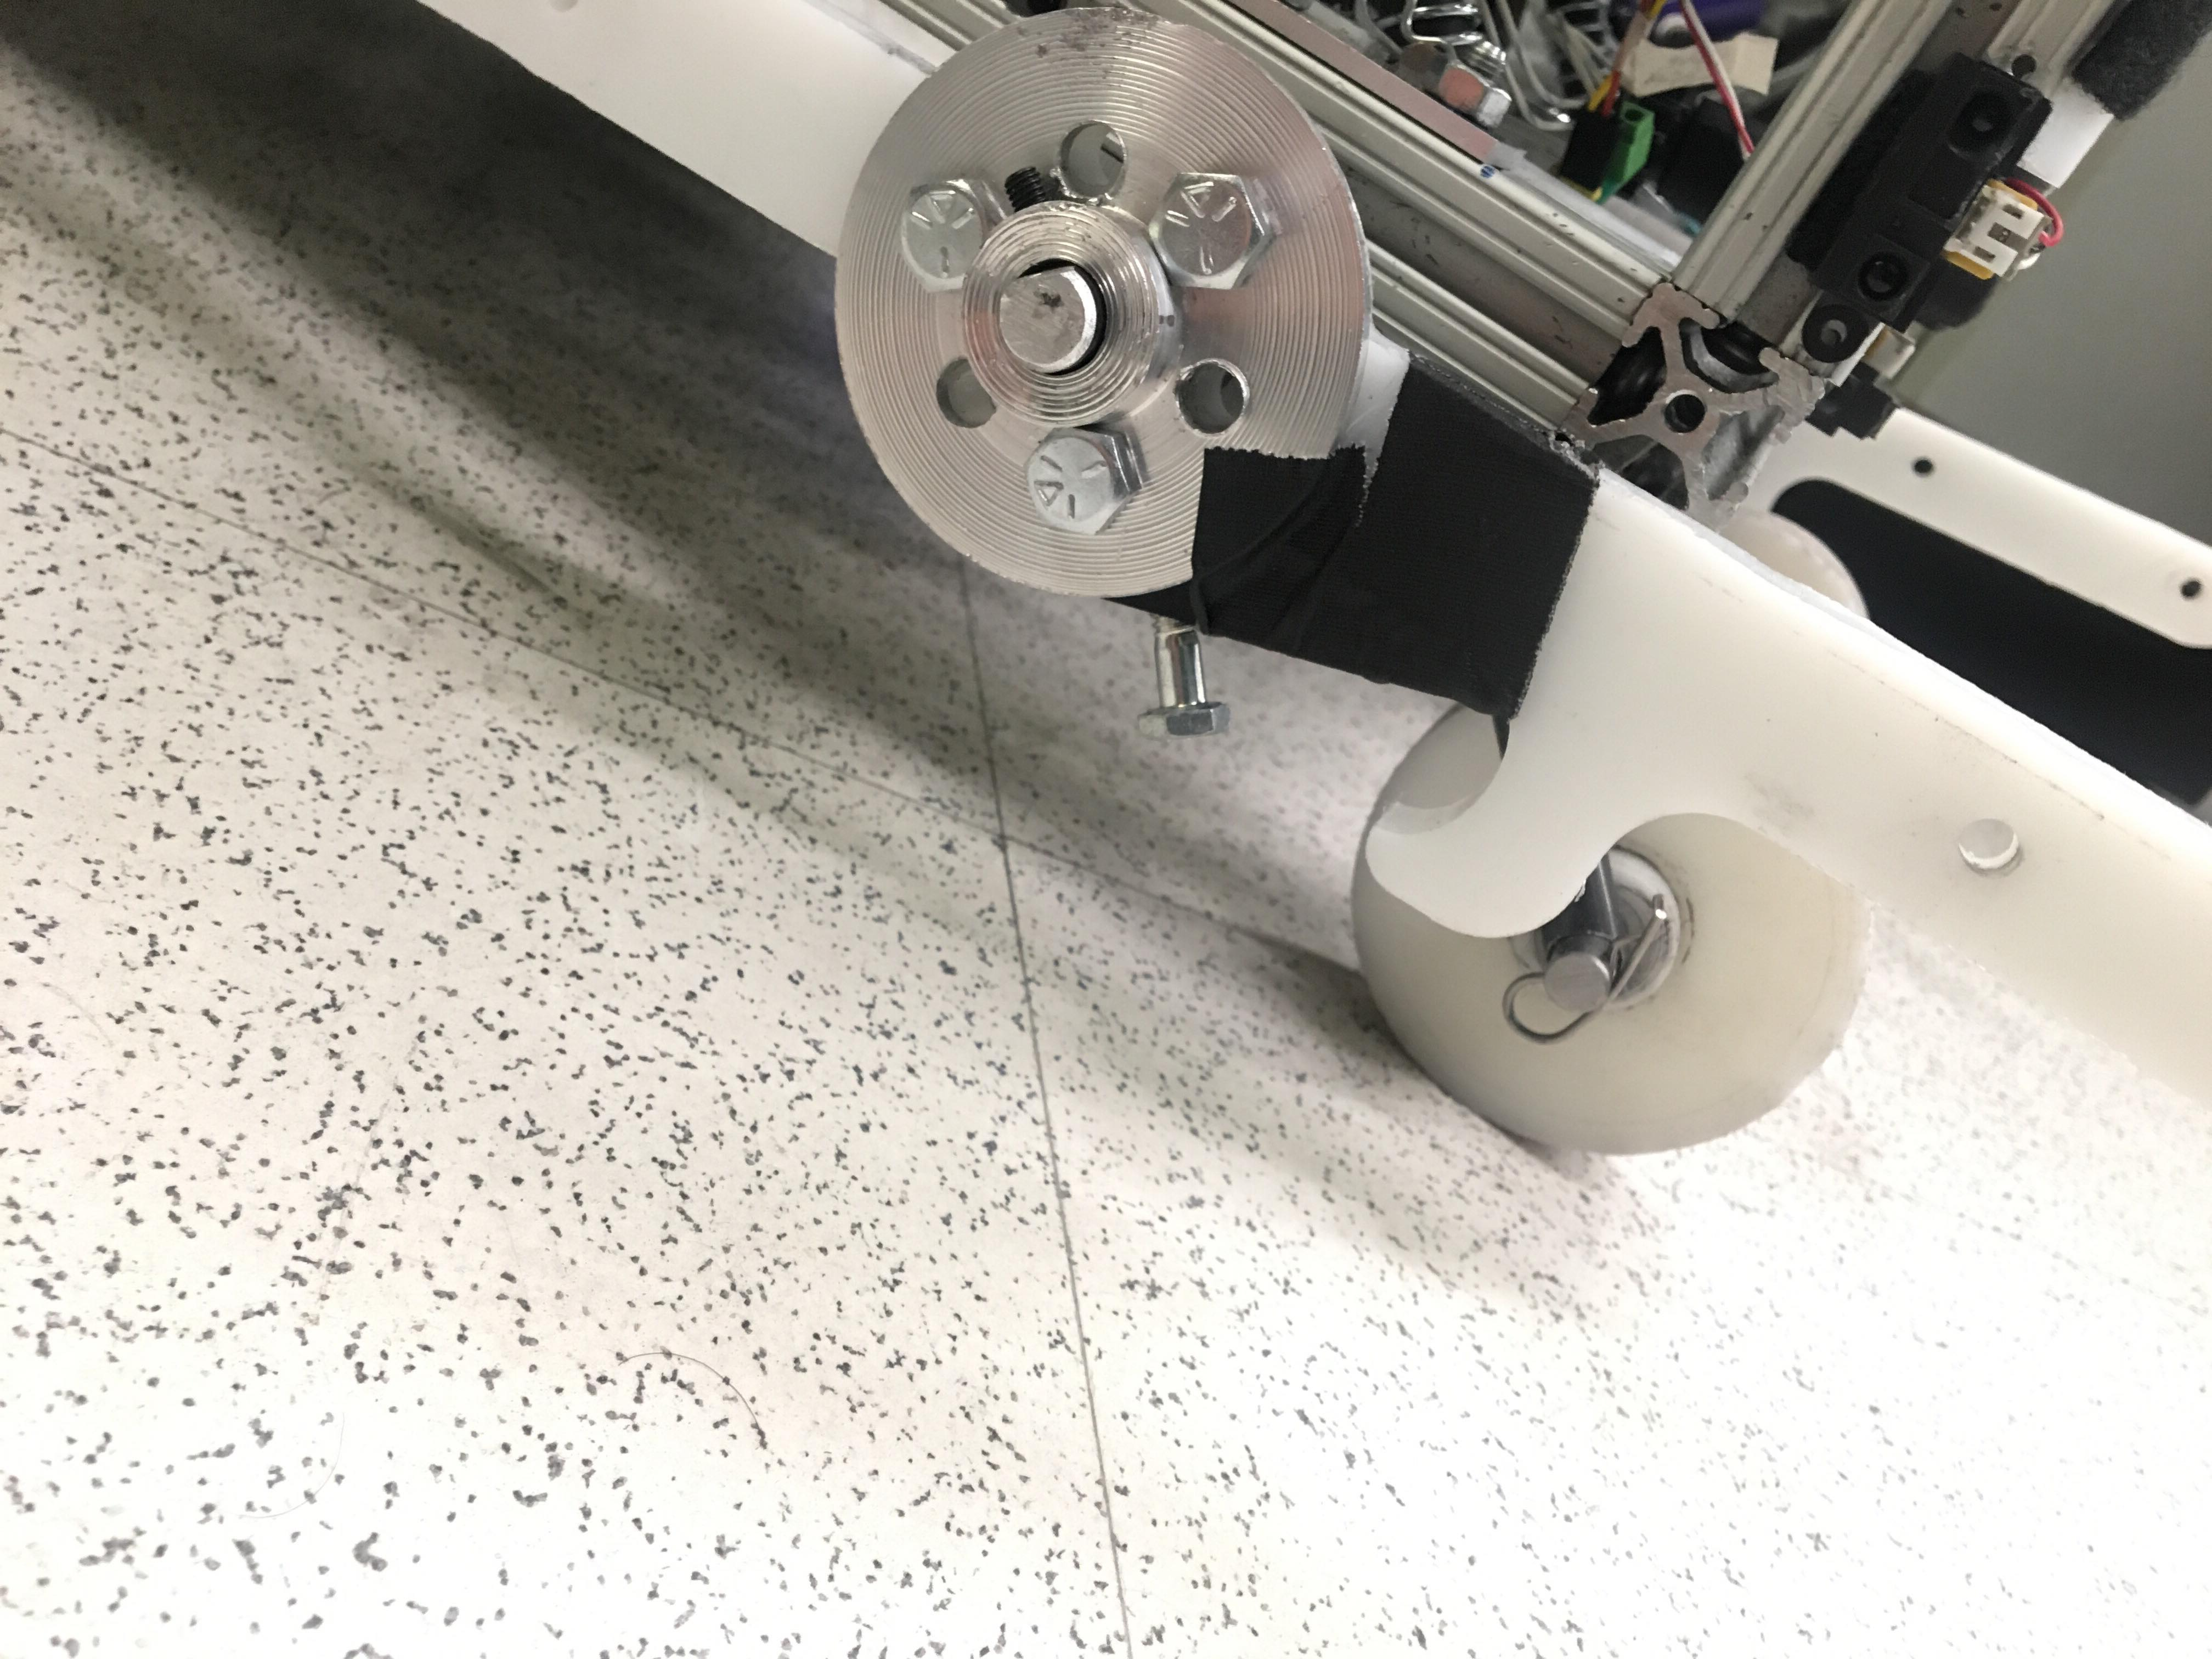
\includegraphics[width=\linewidth]{LiftingArm}
    \caption{Final Lifting Arm Design}
    \label{fig:LiftingArm}
\end{figure}


Having come up with a design for the wall traversal, the SaRRchaeologists also spent time researching other critical design components. From the videos, it became clear that a simple medkit gripper design consisting of a V-shaped protrusion on a rotating arm would be sufficient for picking up and depositing the medkit. It was also clear, however, that the inclusion of a bracket to hold the medkit in place during the course would be necessary in order to prevent it from being dislodged during the violent drop from the wall. A CREO model of the medkit arm is shown in Fig. \ref{fig:MedkitArm}.


The SaRRcheaologists sought to design a SaRR that could not only complete the required tasks, but could do so in an interesting and innovative way that was not reliant on overly complex and failure-prone mechanisms. By iterating through many different geometries for the chassis, front fork assembly, and lifting arms, an innovative, functional design was achieved. In order to maintain the maneuverability of the SaRR through the course, and to keep it from reaching too steep an angle coming off the wall, the chassis was designed to be just long and wide enough to accommodate all the required parts and controlling mechanisms, and no larger. Additionally, emphasis was placed on choosing tires with enough traction and height to aid the SaRR in getting over the wall when working in concert with the lifting arms. Finally, design aspects were chosen to increase the robustness of the SaRR. The frame was designed using 80/20 aluminum extrusion to allow for easy, secure mounting of various components, and to distribute any forces and impulses from the weaker polycarbonate and acrylic sheets to the stronger frame.
The T-slotted 80/20 frame also increased the modularity of the SaRR, so that parts could be moved or replaced with ease. Additionally, in order to reduce the strain on the SaRR each time it dropped off the back of the wall, the front wheels were mounted at a 45 \degree angle to the frame, with shock-absorbing springs mounted onto the supporting forks (Fig. \ref{fig:FrontFork}). The air-filled rear tires were also intended to act as shock absorbers for the back of the robot.

\subsection{Successes and Failures}
As can be expected in any prototyping process, the SaRRchaeologists ran into a number of issues throughout the construction and testing of the robot. One issue that occurred repeatedly involved the shearing of various pins and shafts in the gearboxes. A number of factors contributed to these breakages: severe shocks to the rear wheels upon impact from driving over the walls, and repeated impacts directly to the pins due to imprecise manufacturing that resulted in the side of the gears hitting the pins each time the wheel changed direction. The problem was eventually solved by drilling new holes that were better sized to the pins, and putting in solid dowel pins rather than hollow roll pins.


Additionally, the plastic miter gears initially chosen by the SaRRchaeologists failed after just a few hours of usage, with several of the teeth shearing off completely. Unfortunately, the timing of this failure prevented the team from accomplishing the speed trial milestone on time. After this setback, the team ordered a replacement set of miter gears made of 1144 carbon steel. These miter gears have a yield strength of 620 MPa, and the absolute maximum stress expected on the gears was just under 17 MPa. As expected, these new gears remained completely intact during the usage of the SaRR. These calculations are located in Section \ref{fig:GearStress}.

The SaRRchaeologists where ultimately successful in their attempt to design a sturdy and robust SaRR. Multiple drop tests, as well as accidental inversions during failed autonomous wall traversals proved that the frame of the robot was more than capable of withstanding significant force without breaking or buckling, and the other components were mounted in a way that allowed them to survive large impacts, with only the light sensors mounted to the front of the chassis sustaining damage during an inversion.

An unforeseen problem that the SaRRchaeologists faced was the shifting of the center of gravity going over the wall upon picking up the medkit. Due to the order of the milestones, the lifting arms were designed and tested successfully before the medkit arm assembly was mounted, and while DynaSaRR could easily traverse the wall without the added weight of the medkit, upon picking it up, the weight was shifted too far back and the robot was unable to make it over the final part of the wall, even with the hooks designed for this purpose. A variety of solutions were tested, including adding steel ballast to the front of the robot to shift the center of gravity forward in the hopes of tipping the robot over the wall at the top. Ultimately, success was achieved by adding a bolt to each lifting arm, sitting just in front of the hooks. This bolt levered the circular hub of the arm up, and then slipped forward and caught on the lip of the wall, pulling the robot over as shown in Fig. \ref{fig:bolts}.

Additionally, the SaRRchaeologists had many hardware failures that halted the testing process and adversely affected performance on testing day. The right rear wheel motor (a Vex Mini CIM motor) intermittently stopped responding, but as the problem was seemingly random and difficult to replicate on command, the various fixes attempted (including replacing the snap ring holding the shaft to the gears, replacing the shaft altogether, changing the wires and pins, and replacing the motor controller) failed to reliably fix the problem. It was also difficult to find light and proximity sensors that performed reliably--for example, the day before Demo Day, the SaRRchaeologists noticed that the two light sensors (which had worked well in the past) were reading dramatically different values from each other and did not respond similarly to variations in brightness. This was remedied by testing various sensors and adjusting their variable resistance switches so that they performed more similarly, but the problem was never fully resolved.

Finally, a large unforeseen problem related to the battery life of the drill batteries. The SaRRchaeologists had not initially accounted for not being able to test for extended periods of time due to quick draining of the batteries and poor performance as soon as their level of charge dropped below its peak. This introduced reliability issues in the code--a code that worked at the beginning of testing would have to be adjusted by the end (specifically, the power output to the motors each time the robot was intended to turn had to be increased), as the weaker batteries resulted in drastically different driving performance. However, this new code would then perform poorly the next day on fresh batteries. It appeared that DynaSaRR drained the batteries much faster than expected and performed surprisingly poorly on even half-charged batteries. Were this robot to be improved and rebuilt, managing energy use would be a main concern of the group.

\begin{figure}[ht]
    \centering
    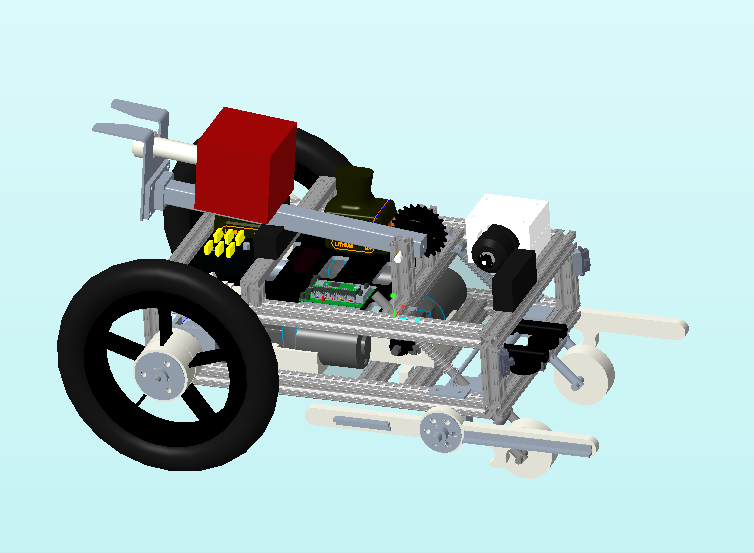
\includegraphics[width=\textwidth]{new_sarr.PNG}
    \caption{DynaSaRR Schematic}
\end{figure}
\section{Project Management}

\subsection{Team Roles}
%{\Large \textbf{Team Roles}}

\addcontentsline{toc}{section}{Team Roles}
\section*{Team Roles}

% \begin{minipage}[t]{0.4\textwidth}
%     \begin{itemize}
%     \item Column 2 content 1
%     \item Column 2 content 2
%     \end{itemize}
%   \end{minipage}

\begin{center}
\resizebox{\textwidth}{!}{
\begin{tabular}{ |c|c|c|c| } 
    \hline
    Name & Specialty & Responsibilities & PDR Contributions \\
    \hline
    Jackson Artis & CAD Work & cell3 & cell4\\
    \hline
    Morgan Baker & Machining & cell3 & cell4\\
    \hline
    Sam Dale & Coding & cell3 & cell4\\
    \hline
    Alexandra Koskosidis & Team Leader, Analysis & cell3 & cell4\\
    \hline
    Alex Rogers & CNC & cell3 & cell4\\
    \hline
    Evan Quinn & Electrical Engineering & cell3 & cell4\\
    \hline
    
\end{tabular}}
\end{center}

\vfill % Fill the rest of the page with whitespace
\newpage

\subsection{Personnel}
Alexandra Koskosidis: Team Leader, Coding\\

    It was the primary responsibility of the Team Leader to direct the individual members of the group and the direction of the project as a whole. The Team Leader worked with the members of her group to ensure all necessary tasks were undertaken and completed by delegating sub-projects and setting completion date objectives. She scheduled team meetings, posed concerns to the group for discussion, and updated all members on progress. Additionally, the role of Coding Specialist was fulfilled by writing, debugging, and managing the completion of code for all autonomous parts of the SaRR. \\
    
Alex Rogers: CNC, Hardware Systems\\

    The CNC Specialist was mainly responsible for CNCing all CAD parts by creating mill volumes and designing tool paths. The CNC Specialist worked closely with Al to check pieces and reserve space in the CNC. Thus, he was also very involved in the main CAD model, adjusting dimensions of parts and making final assemblies to accommodate design changes. The role of Hardware Systems Specialist consisted of organizing electronics, mounting sensors, debugging potential motor and sensor issues and ensuring proper construction of the SaRR. This role worked closely with the Coding Specialist to assist with electronics and sensor readings. \\
    
Evan Quinn: Manufacturing\\

    The Manufacturing Specialist was tasked with manually machining parts such as the axles, couplings, gearboxes, and gears, and working in tandem with the Hardware Systems Specialist to assemble the robot and connect motors and other electrical components. He worked closely with the Coding Specialist to ensure the functionality of the proximity and light sensors.\\
    
Jackson Artis: CAD Modeling\\
    
    The CAD Specialist oversaw the CREO modeling process, in which design ideas were transformed into CAD models to allow for clear dimensioning and subsequently accurate manufacturing of parts. The CAD specialist was responsible for making sure the CREO model was in a state that was easily and readily transferable to the manufacturing process. What's more, he was responsible for aiding in and overseeing all CREO simulations and analyses including various buckling analyses and center of gravity calculations. \\ 

Morgan Baker: Analysis, Manufacturing Assistant\\

    The Analyst was responsible for completing free-body diagrams, calculations regarding torque, center of gravity, static stability margins, and stress on crucial components to ensure that the team avoided major mechanical failures. The Manufacturing Assistant was responsible for assisting with the machining of and overseeing of all machined parts. The Manufacturing Assistant worked closely with the Manufacturing and CNC Specialists to ensure that the best possible methods were used to create parts.\\
    
Sam Dale: Design, Electronics\\

    The Design Specialist focused on the development and implementation of mechanical design and functionality, primarily during the initial design phase of the project. While design decisions were ultimately made in full-team brainstorming sessions, the Design Specialist spearheaded these initiatives and oversaw the creation of the initial CAD models. The Electronics Specialist role included planning out electronic placement, soldering and wiring all the components, ensuring that they were connected properly, and debugging electronics issues as they arose.
    

\subsection{Schedule and Tasks}

The schedule for the whole project is outlined below, with approximate hours spent on each task and commentary about success provided.

\begin{itemize} 
\item Course Milestone: Demonstrate Open-Loop Drive-train (24:35)
\begin{itemize}
\item CNC motor holders, cut axles, assemble belt tighteners
\item Wired breadboard, soldered wires
\item Programmed controller, connected to breadboard
\item The initial wiring was not done by the team, but rather by members of a lab group, and was not considered up to the SaRRchaeologists' standards. Most of the wires were soldered again, and connections were remade.
\item Due: Week of Feb. 25th
\item Completed: March 1, 2019--On time
\end{itemize}
\end{itemize}
\begin{itemize}
\item Course Milestone: Closed-Loop Navigation to Light Source (52:05) 
\begin{itemize}
\item Attached light and proximity sensors 
\item Connected sensors to outputs, read sensors 
\item Wrote code to read sensor outputs respond appropriately
\item Due: Week of Mar. 4th
\item Completed: March 7th, 2019--On time
\end{itemize}
\end{itemize}
\begin{itemize}
\item Team Milestone: Finalize Design, Parts Order
\begin{itemize}
\item Individual brainstorming, idea proposals and deliberation
\item CAD model and cardboard prototyping
\item Bill of Materials
\item Initial parts order
\item Motor torque and gearing calculations
\item Due: March 11
\item Completed: March 24th, 2019--Later than desired (partly due to Spring Break)
\end{itemize}
\end{itemize}
\begin{itemize}
\item Team Milestone: Begin Assembly (84:30)
\begin{itemize}
\item Manufactured gearbox components 
\item Calculations for center of gravity, lifting arm torque, energy use, etc.
\item Due: Week of March 24th
\item Completed: On time. Sufficient work was completed to declare this task fulfilled
\end{itemize}
\end{itemize}
\begin{itemize}
\begin{itemize}
\item Course Milestone: PDR (50:40)
\begin{itemize}
\item Due: Apr. 4
\item Completed: Apr. 4, 2019--On time
\end{itemize}
\end{itemize}
\item Course Milestone: Speed Trial (228:00)
\begin{itemize}
\item Finished chassis assembly
\item Assembled gearbox, mounted motors, connected wheels 
\item Attached and secured hardware
\item Due: Apr. 5
\item Completed: Apr. 8, 2019--One day late
\item The Speed Trial milestone was met the Monday after the due date. The deadline was missed due to the shearing of the plastic driving gears several hours before the trial.
\end{itemize} 
\end{itemize}
\begin{itemize}
\item Course Milestone: Open-Loop Wall Traversal (108:30)
\begin{itemize}
\item Manufactured lifting arms 
\item Mounted lifting motor and driving sprockets
\item Programmed controller
\item Due: Apr. 12
\item Completed: Apr. 12, 2019--On time
\end{itemize}
\end{itemize}
\begin{itemize}
\item Course Milestone: Open-Loop Object Retrieval/Placement (70:30)
\begin{itemize}
\item Machined medkit arm
\item Mounted and attached medkit motor 
\item Due: Apr. 19
\item Completed: Apr. 19, 2019--On time
\end{itemize}
\end{itemize}
\begin{itemize}
\item Course Milestone: Closed-loop Object Placement (92:00)
\begin{itemize}
\item Mounted light sensors from sample robot
\item Modified sample robot code to work with DynaSaRR
\item Began programming for autonomous chute navigation
\item Due: Apr. 26
\item Completed: Apr. 26, 2019--On time
\end{itemize}
\end{itemize}
\begin{itemize}
\item Team Milestone: Closed-loop Chute Navigation (76:30) 
\begin{itemize}
\item Mounted side proximity sensors
\item Completed code for closed-loop chute navigation
\item Some issues were encountered due to unpredictable performance as battery charge decreased and right rear wheel motor unreliability
\item Due: May 3
\item Completed: May 3, 2019--On time
\end{itemize}
\end{itemize}
\begin{itemize}
\item Team Milestone: Autonomous Wall Traversal, Successful Course Completion, Repair Mechanical Issues (146:34)
\begin{itemize}
\item Wrote and debugged autonomous wall traversal code
\item Joined autonomous portions of code
\item Repaired mechanical issues with permanent solutions to ensure proper functionality going into competition
\item Due: May 10
\item Completed: N/A
\item The SaRRchaeologists were unable to produce reliable code for the autonomous portion of the course. While each individual component worked individually (and the chute and light/placement codes were able to work in tandem), the unreliability of robot performance during testing (due to dropping charge and mechanical problems) prevented the completion of robust code.
\end{itemize}
\end{itemize}
\begin{itemize}
\item Course Milestone: Demo Day, May 14th
\begin{itemize}
\item Demonstrated search and rescue capabilities of DynaSaRR
\item Unfortunately, the results of this demonstration proved to be disappointing. Successes, failures, and potential explanations are discussed in section 7.
\end{itemize}
\end{itemize}
\item Course Milestone: FDR
\item Due: May 14
\item Completed: May 14th, 2019--On time

\subsection{Key Tasks with Leaders}

\begin{table}[htv]
\resizebox{\textwidth}{!}{%
\begin{tabular}{lll}
\textbf{Key Tasks}                          & \textbf{Task Leader} & \textbf{Completed} \\
Autonomous Light Navigation--Sample Robot   & Sam Dale             & 3/7/19             \\
Finalize Preliminary Design                 & Sam Dale             & 3/29/19            \\
Assembly of SaRR                            & Evan Quinn and Alex Rogers          & 4/4/19             \\
PDR                                         & Jackson Artis        & 4/5/19             \\
Speed Trial                                 & Evan Quinn & 4/8/19             \\
Open-Loop Wall Traversal                    & Alex Rogers          & 4/12/19            \\
Open-Loop Medkit Retrieval and Placement   & Morgan Baker          & 4/19/19            \\
Closed-Loop Light Tracking and Medkit Placement & Sam Dale             & 4/26/19            \\
Closed-Loop Chute Navigation                & Alexandra Koskosidis & 4/30/19            \\
Closed-Loop Continuity                      & Alexandra Koskosidis & 5/10/19            \\
Final Presentation                          & Morgan Baker         & 5/13/19            \\
FDR                                         & Jackson Artis        & 5/14/19           
\end{tabular}%
}
\end{table}



\subsection{Management Approach}

The team recognized that the most important part of project management is constant, effective communication. Before any design or manufacturing began, the group set up a chat on Facebook Messenger, which allowed all members to collaborate at the same time from their phone or laptop, and actively identify who has seen the messages and who has not (unlike text message). Furthermore, a WhenIsGood form was compiled to identify the time slots during which each team member would be available. This form made it easy for the Team Leader to organize team meetings and assign work to people by the hour. Team meetings were scheduled during the l period every Monday, which was considered the Team Lab Time. Any other meetings were scheduled as needed. Team members recorded their work hours in the Time Sheet after any time spent working on the project. This log included a description of the task worked on, which held team members accountable for their work and allowed for an ongoing tally of the hours spent on each task and on the project as a whole.

Initially, tasks were managed rather informally, with team members sending the times they planned to work that week into the group chat and the Team Leader assigning them the appropriate tasks based on that scheduling. Unfortunately, this strategy proved inefficient, as high-priority tasks assigned in a certain order would end up being completed later than expected due to unforeseen changes in team members' availability, and therefore delayed subsequent tasks.

Following the SaRRchaeologists' failure to meet the speed trial milestone on time, a long team meeting was held in which each team member was encouraged to speak freely and bluntly (though constructively) about challenges faced and mistakes made by each person, as well as suggestions for improvement, which included comments on work assignment strategies, disorganization and quality of work. This conversation was helpful for discussing major themes that Frank Ryle presented in lecture such as conflict approaches, risk analyses, and viewing group members as stakeholders that were near as important as other stakeholders like Professor Nosenchuck and Aaron. As a result of this discussion, the management strategy changed completely for the rest of the semester. This meeting saw the creation of an organized, color-coded To Do List, in which tasks could be entered and deadlines assigned. The list had two main features that drastically improved the efficiency of the group's organization: first, tasks could be assigned to individual team members, and comments could be recorded next to the task to make the information easily accessible. Second, the list could was sorted by priority, and the dependency of certain tasks on those before them was made clear. This proved to be much more successful, as it placed the onus on individual team members to see their upcoming assignments and plan their work hours accordingly. Additionally, it allowed for anyone finishing their assignment early to immediately begin work on the next task, rather than having to discuss in the group what was next to be done.


A major issue anticipated by the SaRRchaeologists was manufacturing and coding errors made as a result of fatigue and carelessness after many hours of work. As a result, team members attempted to work in pairs or groups of three whenever possible so that a partner could provide a "sanity check" and catch any overlooked problems in the manufacturing of a part or the writing of code. On the other hand, with the exception of design discussions, the SaRRchaeologists tried to avoid having more than two or three members working on the same task at once, as this frequently resulted in one or more members watching the others complete the task and making inefficient use of their limited time.

Any personal issues or friction that arose were resolved with promptly--team members were open with each other and communicated in a direct, constructive way, pointing out any practices that were not ideal and suggesting improvements and ways to remedy mistakes, while also acknowledging strengths and successes. Smaller design problems were generally resolved on the spot as they arose by whichever team members were working on that task, but larger changes were always brought to the whole group for discussion, and not implemented until all 6 group members were fully on board. If someone disagreed with a design decision or preferred another method, discussion continued until they felt comfortable with the solution and were ready to help implement it. Overall, the group worked cohesively, with no major issues and successful communication.

\clearpage

\subsection{Total Time}
% \begin{center}
% \begin{tabular}[ |c|c|c| ]
%     \csvautotabular{./resources/total-time_v1.csv}
%     \caption{Total time spent working on the project for each team member.}
% \end{tabular}
% \end{center}

\begin{table}[htv]
\centering
\begin{tabular}{l|l|l|}
\hline
\multicolumn{1}{|l|}{\textbf{Team Member}} & \textbf{Hours Worked} & \textbf{Percent of Total} \\ \hline
\multicolumn{1}{|l|}{Alexandra Koskosidis} & 185:50 & 19.67\% \\ \hline
\multicolumn{1}{|l|}{Alex Rogers} & 142:20 & 10.07\% \\ \hline
\multicolumn{1}{|l|}{Evan Quinn} & 95:30 & 10.11\% \\ \hline
\multicolumn{1}{|l|}{Jackson Artis} & 139:25 & 14.76\% \\ \hline
\multicolumn{1}{|l|}{Morgan Baker} & 140:00 & 14.82\% \\ \hline
\multicolumn{1}{|l|}{Sam Dale} & 241:30 & 25.57\% \\ \hline
 & 944:35 & 100\% \\ \cline{2-3} 
\end{tabular}
\caption{Total time spent working on the project for each team member.}
\end{table}


\clearpage
\section{Detailed Design and Analysis}

The total weight of DynaSaRR with the medkit stowed is approximately 48 lb. In this configuration, the center of mass is 6 in. in front of the back wheel axle and in the center of the chassis (see Fig. \ref{baxle}). 


\subsection{Subsystem Analysis}
Certain sections of the DynaSaRR were identified as subsystems of high import, namely the front wheel forks, the lifting arms, and the medkit arm. These subsystems were chosen due to their propensity to take large impulses and shocks. As such, the SaRRchaeologists determined that if DynaSaRR were to break, it would be at these key points. The following sections represent the analyses of those sections.

\subsubsection{Front Wheel Forks}
The front wheel forks are built from four steel pieces welded together. The HDPE wheel is mounted on an axle supported by the fork (see Fig. \ref{fig:frontforks}). Static and buckling analyses were performed only on the left front wheel fork assembly; as such, only half of DynaSaRR's weight was used for these calculations. Because this subsystem was mirrored across DynaSaRR's center line, the center of mass between the two front wheel forks would simply shift laterally to the center line of DynaSaRR while maintaining the same vertical coordinate.

Figure \ref{fig:displacement} shows that the assembly has a maximum displacement of 1.275e-4 inches. Figure \ref{fig:buckling} shows that a buckling factor of 1948 was predicted by CREO. Based on these simulations, the SaRRchaeologists were able to confidently conclude that the front forks would not be a likely failure mode.

\begin{figure}[hp]
    \centering
    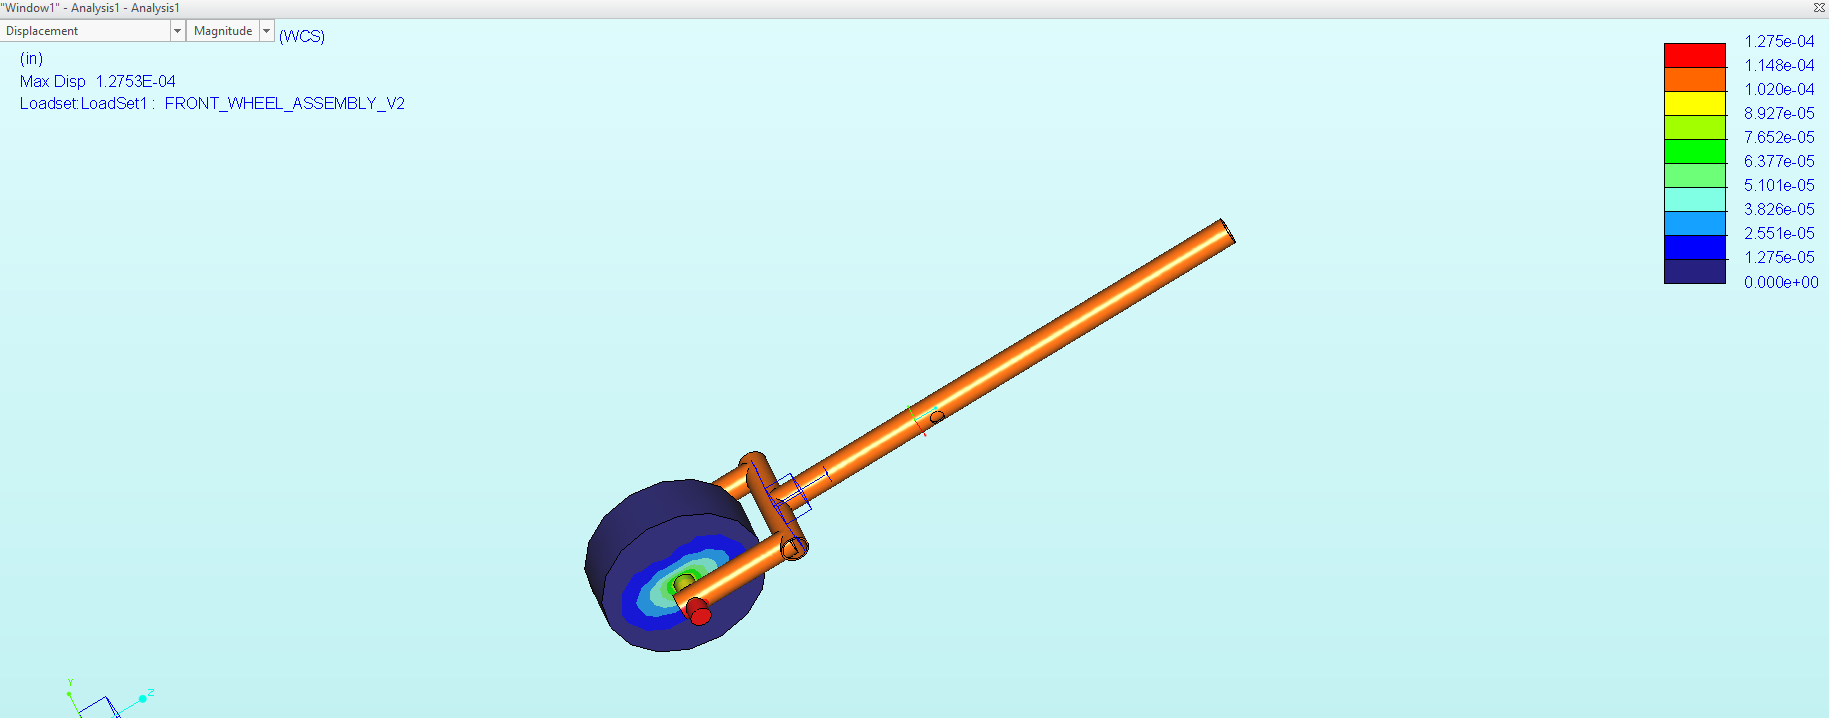
\includegraphics[width=0.4\textwidth]{Images/front_wheel_disp.PNG}
    \caption{Displacement Diagram for Front Wheel Fork Assembly}
    \label{fig:displacement}
\end{figure}
\newpage

\begin{figure}[hp]
    \centering
    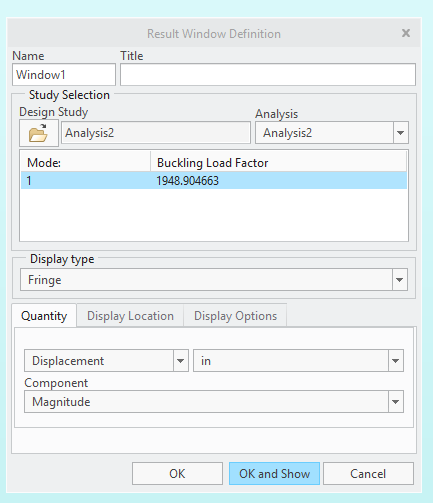
\includegraphics[width=0.4\textwidth]{Images/front_wheel_buckle.PNG}
    \caption{Buckling Factor for Lifting Arm Complex for a load of 25 lbf}
    \label{fig:buckling}
\end{figure}
\newpage

\begin{figure}[hp]
    \centering
    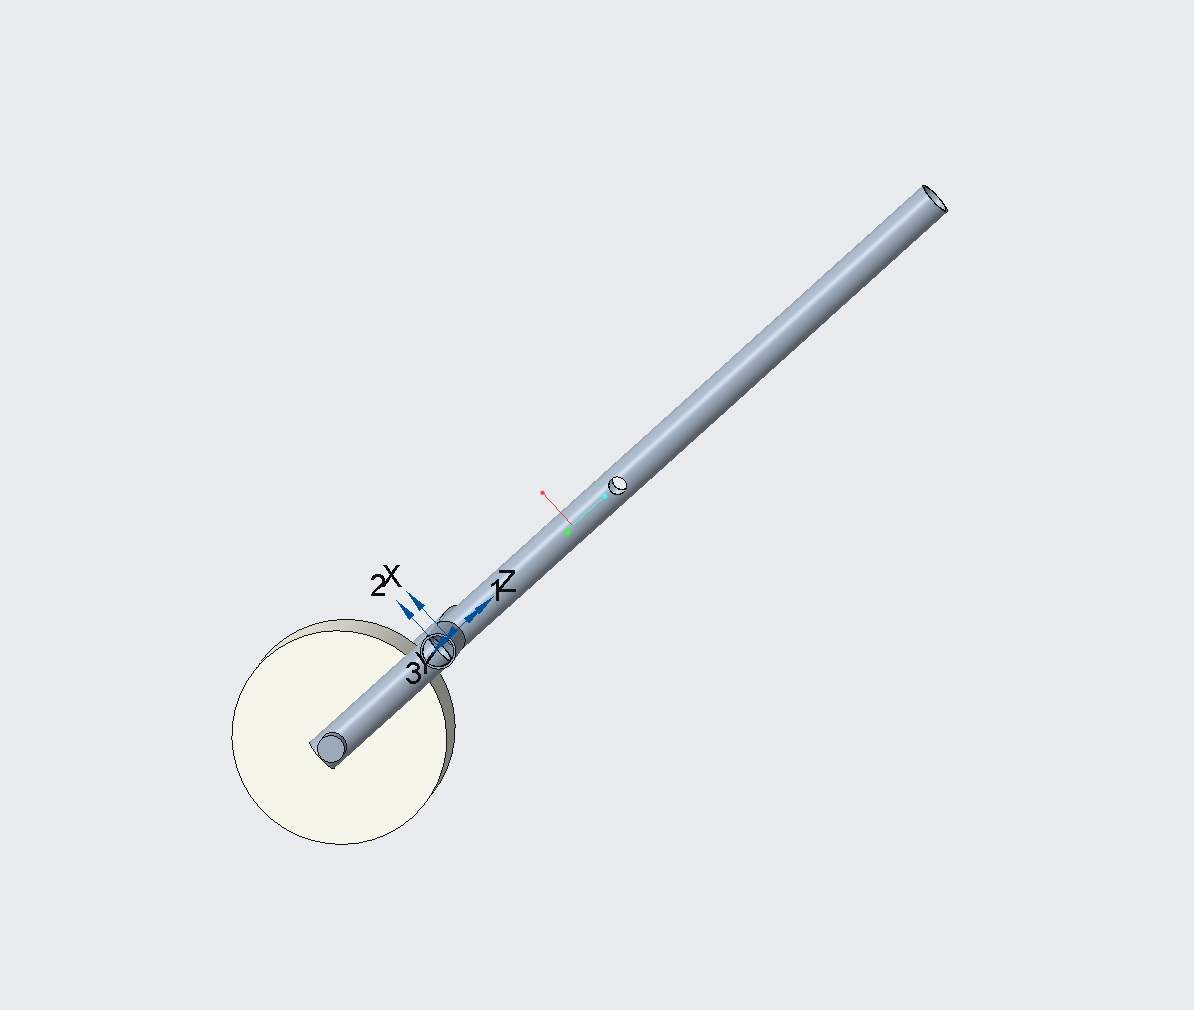
\includegraphics[width=0.4\textwidth]{COM_fork.jpg}
    \caption{Wheel Fork Assembly Center of Mass}
    \label{fig:Center of Mass}
\end{figure}
\newpage


\subsubsection{Lifting Arms}
The lifting arms were made in the CNC from stock HDPE. The gripping plate was also made from an Aluminum 6061 work piece in the CNC. The gripping plate was bolted to the HDPE and then a set screw was used secure it to the axle (for reference, see the Lifting Arm Assembly Drawing in the appendices). Static and buckling analyses were performed on the lifting arm assembly, with only half of DynaSaRR's weight used for these calculations. Because this subsystem was mirrored across DynaSaRR's center line, the center of mass between the two lifting arms would simply shift laterally to the center line of DynaSaRR while maintaining the same vertical coordinate.


Figure \ref{fig:disp2} shows that the assembly has a maximum displacement of .5 inches between the two contact points. Figure \ref{fig:buck2} shows a minimum buckling factor of 4.96. These values show that while the lifting arms were not drastically overengineered, DynaSaRR was unlikely to fail at this point.
\begin{figure}[hp]
    \centering
    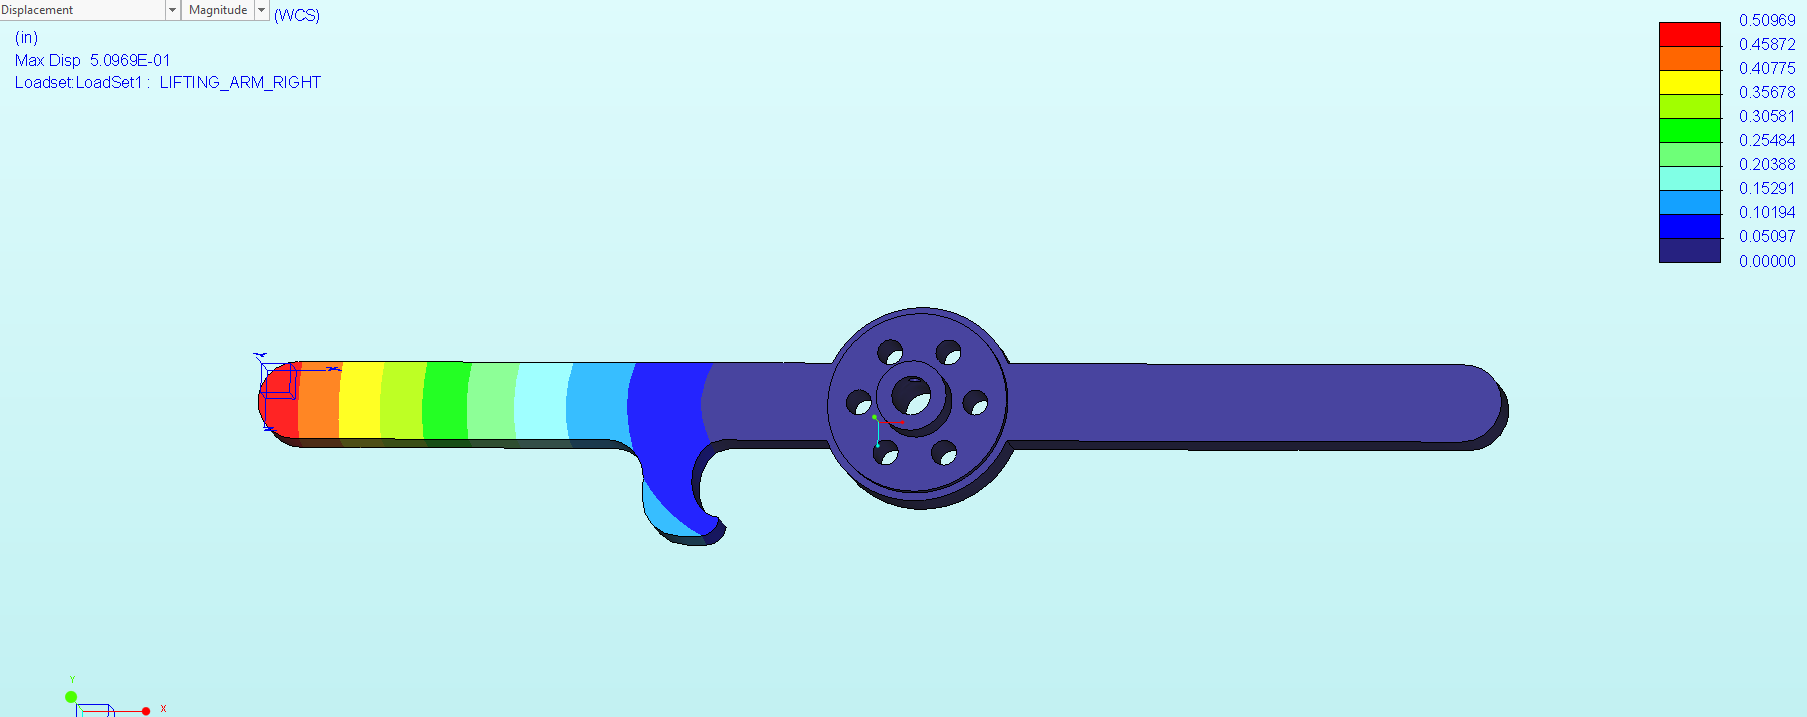
\includegraphics[width=0.5\textwidth]{Images/lifting_arm_final_1_disp.PNG}
    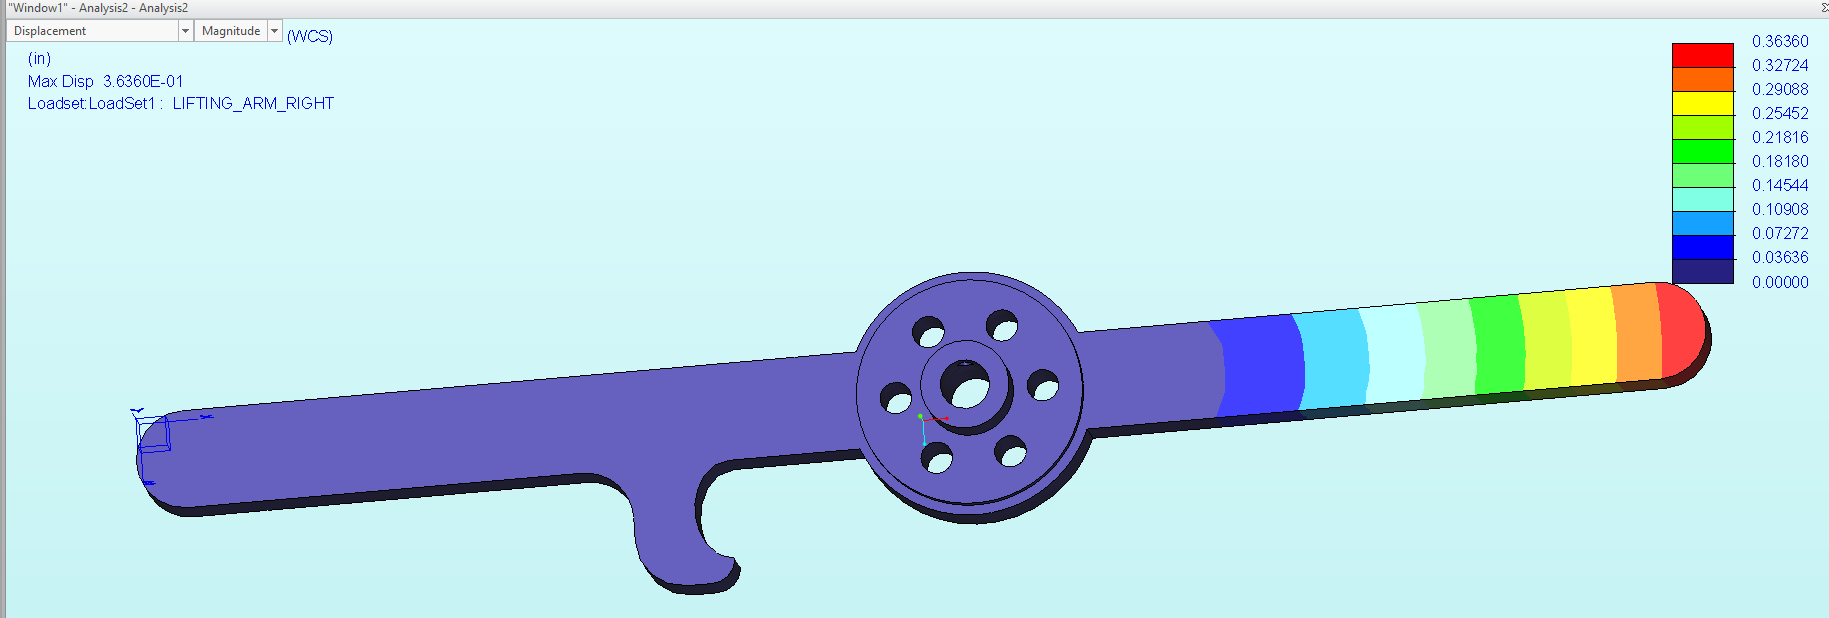
\includegraphics[width=0.5\textwidth]{Images/lifting_arm_final_2_disp.PNG}
    \caption{Displacement Diagram for Lifting Arm Assembly, both points of contact}
    \label{fig:disp2}
\end{figure}
\newpage

\begin{figure}[hp]
    \centering
    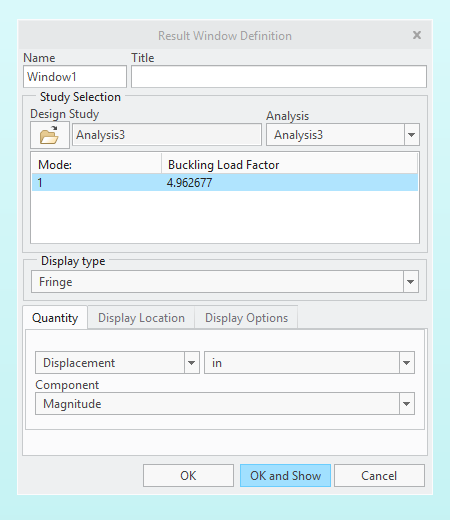
\includegraphics[width=0.25\textwidth]{Images/lifting_arm_final_1_buckle.PNG}
    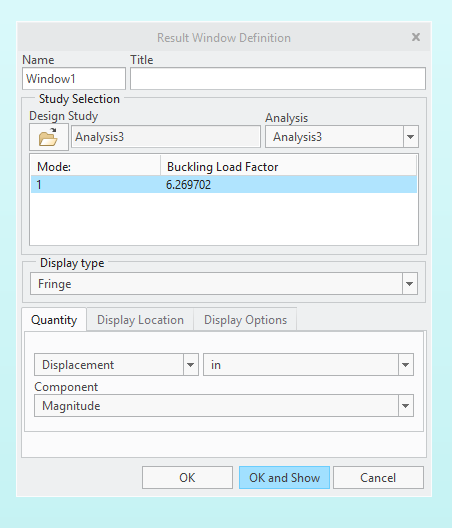
\includegraphics[width=0.25\textwidth]{Images/lifting_arm_final_2_buckle.PNG}
    \caption{Buckling Factor for Lifting Arm Assembly for a load of 25 lbf, both points of contact}
    \label{fig:buck2}
\end{figure}
\newpage

\begin{figure}[hp]
    \centering
    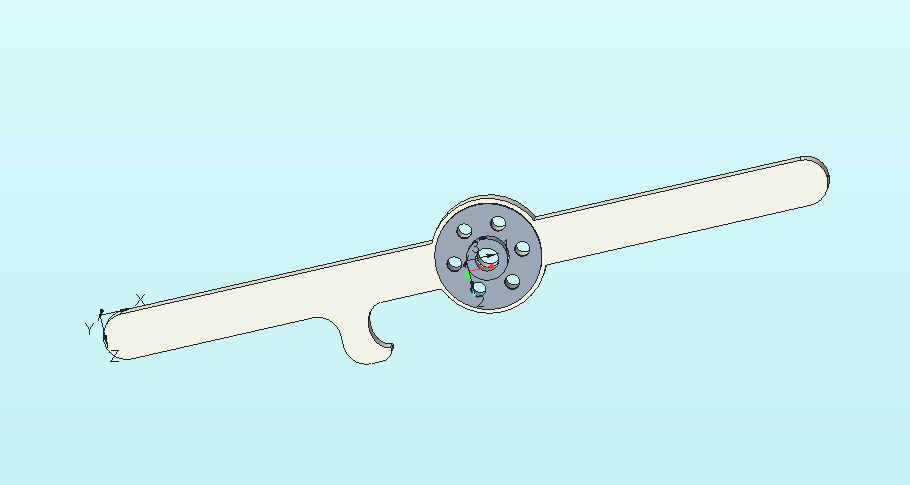
\includegraphics[width=0.5\textwidth]{Capture.PNG}
    \caption{Lifting Arm Assembly Center of Mass}
    \label{fig:FrontFork}
\end{figure}
\newpage

\subsubsection{Medkit Arm}

The Medkit Arm was made from an Aluminum 6061 work piece and an Aluminum 6061 80/20 extrusion. The portion of the arm that grabs the medkit was made in the CNC from a stock Aluminum 6061 piece. The pieces are bolted together (for reference, see Medkit Assembly Drawing). Static and buckling analyses were performed on the Medkit Arm Assembly, with Fig. \ref{fig:disp3} showing a maximum displacement of 0.00366 inches, and Fig. \ref{fig:buck3} showing a buckling factor of 1790.3. These simulations show that this arm was also significantly overengineered for the given medkit, and that it would be virtually guaranteed not to fail.

\begin{figure}[hp]
    \centering
    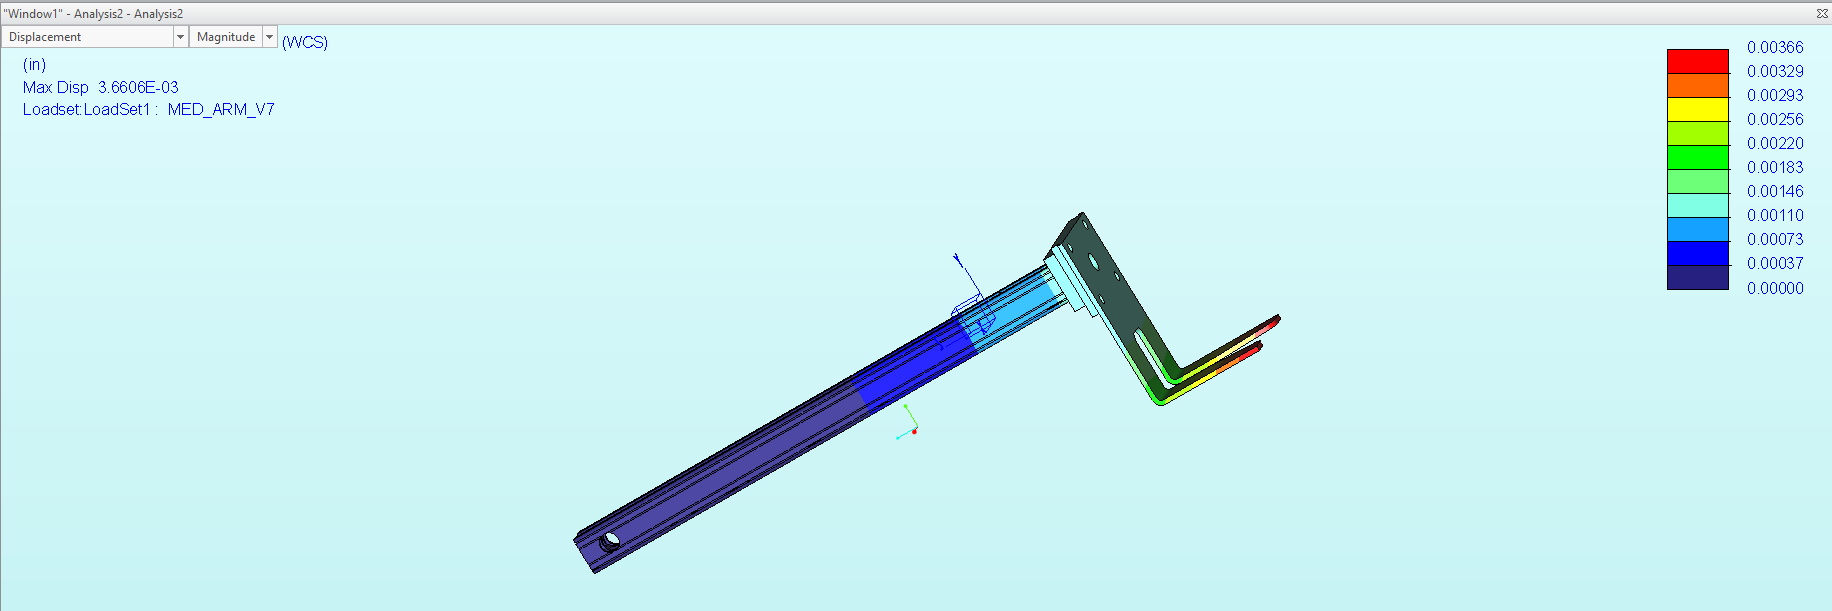
\includegraphics[width=0.4\textwidth]{Images/medkit_displ.PNG}
    \caption{Displacement Diagram for Medkit Arm Assembly}
    \label{fig:disp3}
\end{figure}
\newpage

\begin{figure}[hp]
    \centering
    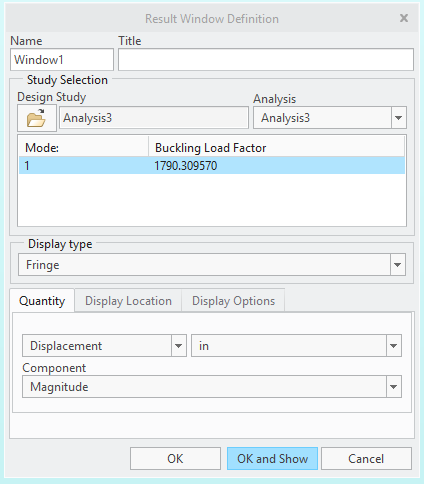
\includegraphics[width=0.4\textwidth]{Images/medkit_buckling.PNG}
    \caption{Buckling Factor for Medkit Arm Assembly for a load of 5 lbf}
    \label{fig:buck3}
\end{figure}
\newpage

\begin{figure}[hp]
    \centering
    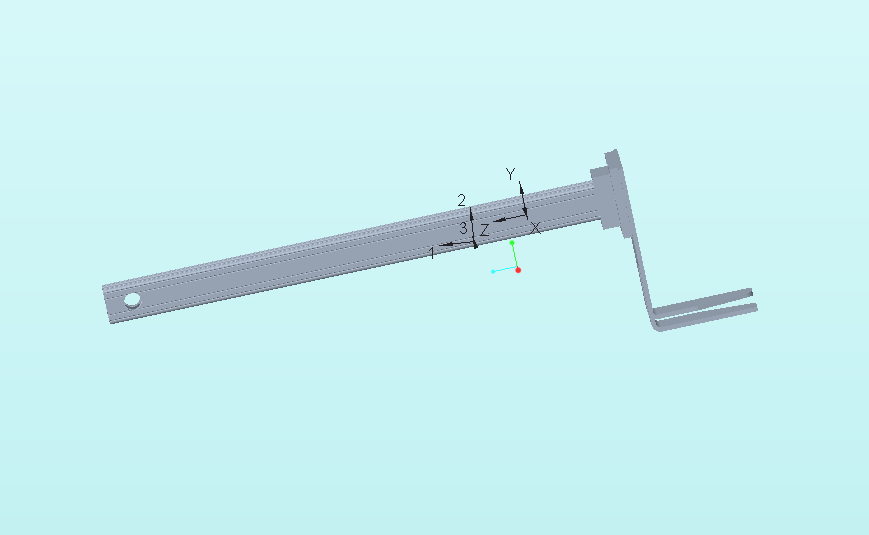
\includegraphics[width=0.5\textwidth]{Images/medkit_COM.PNG}
    \caption{Medkit Arm Assembly Center of Mass}
    \label{fig:MedkitArm}
\end{figure}
\newpage








\begin{figure}[hp]
    \centering
    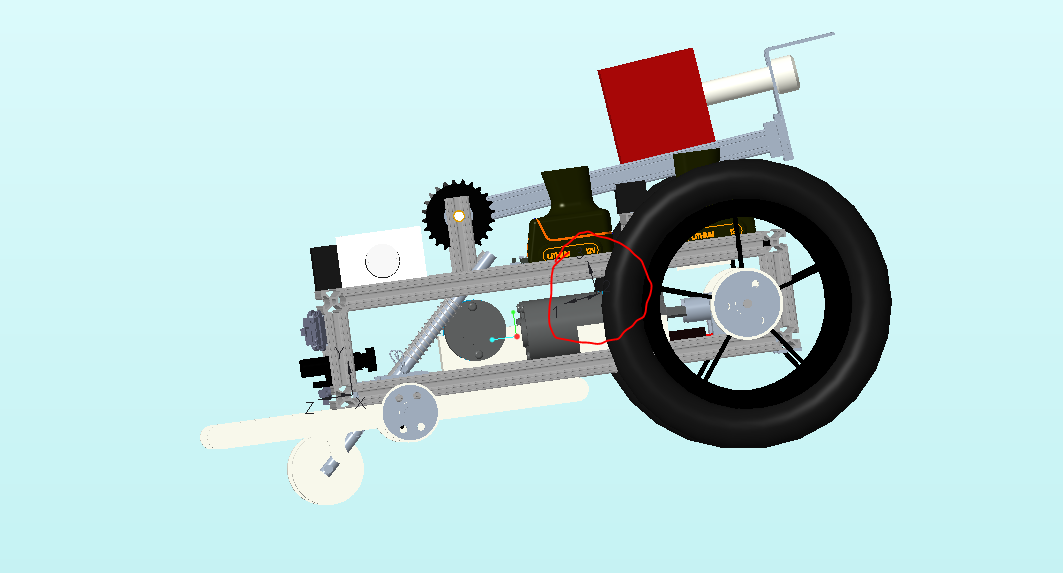
\includegraphics[width=0.8\textwidth]{Images/assemblyCOM.PNG}
    \caption{Fully Assembled DynaSaRR with Isolated Center of Mass}
\end{figure}

The free body diagrams of the configurations mentioned previously are illustrated in figures \ref{fig:analysis1_medkitstowed} and \ref{fig:analysis2_liftingmedkit}.  In both figures, it can be seen that the back of DynaSaRR supports more weight than the front.  This is useful in the medkit retrieval, as the calculations show that it would take a load of 69.3 lb at the end of the medkit arm for DynaSaRR to tip over.

\label{fig:analysis1_medkitstowed}
\begin{figure}[hp]
    \centering
    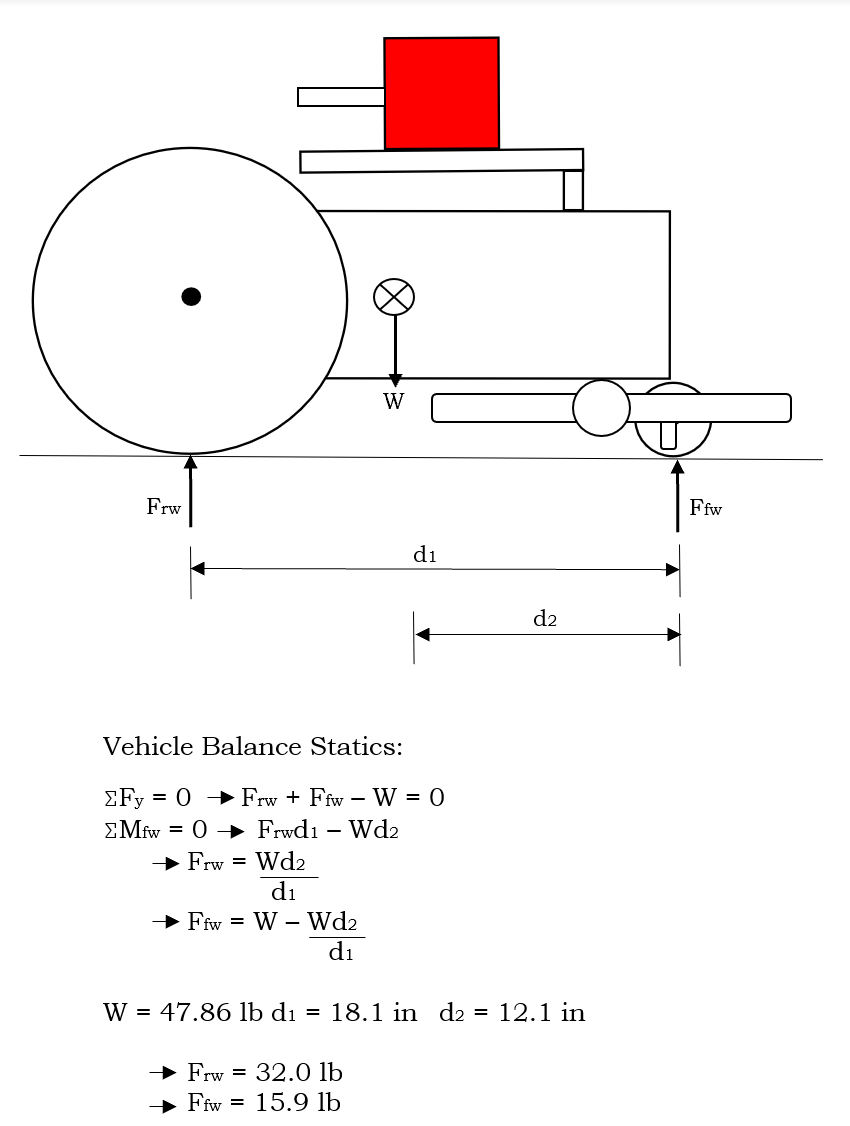
\includegraphics[width=0.8\textwidth]{Images/analysis1_medkitstowed.png}
    \caption{Free Body Diagram and Calculations for DynaSaRR with Med Kit Stowed}
    \label{fig:analysis1_medkitstowed}
\end{figure}
\vfill
\newpage

\label{fig:analysis2_liftingmedkit}
\begin{figure}[hp]
    \centering
    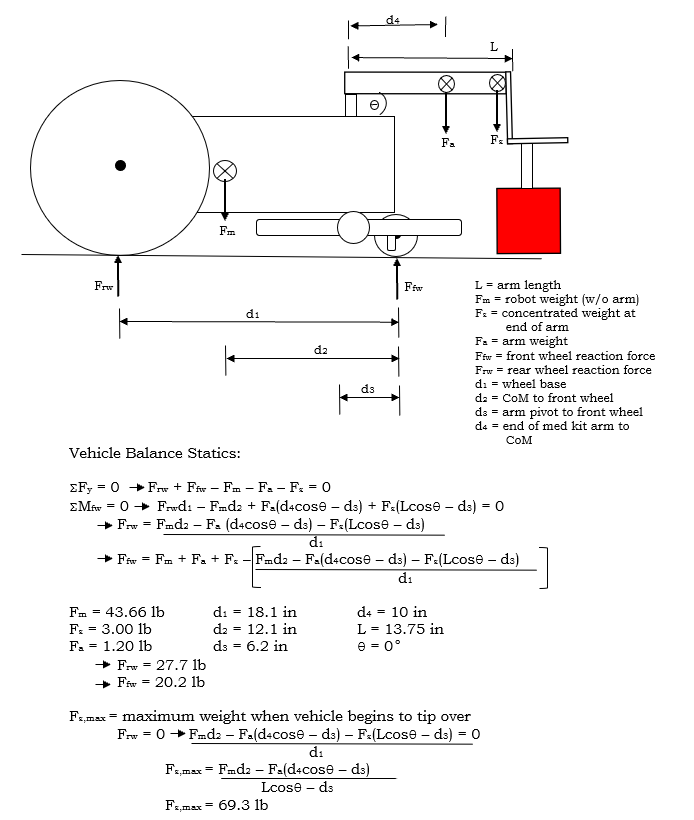
\includegraphics[width=0.8\textwidth]{Images/analysis2_liftingmedkit.png}
    \caption{Free Body Diagram and Calculations for DynaSaRR when Beginning to Lift Med Kit}
    \label{fig:analysis2_liftingmedkit}
\end{figure}
\vfill
\newpage


In designing a medkit retrieval mechanism, the primary considerations were a gripper that would not require tremendous precision in order to pick up the med-kit handle, and a mechanism to secure the med-kit into place after it was lifted onto the SaRR, so that it would not fall out during the wall traversal or other sections of the obstacle course. To fit the first consideration, DynaSaRR lowers an arm with a flat gripper component at the front. The gripper is composed of two triangular pieces of aluminum that funnel the handle of the medkit into the triangular space between them and then into a slot cut into the gripper. The V-shaped gripper is intended to minimize the precision required in driving up to the med-kit by providing a large capture area. The arm then rotates upward, with the med-kit pivoting in the gripper slot until it falls into a bracket mounted on the underside of the arm intended to secure it.

The SaRRchaeologists decided to utilize the same Vex Mini CIM Motor for the lifting arms as was used for the back wheels. The published data shows a stall torque of 1.41 Newton-Meters. The SaRRchaeologists used a conservative estimate of 1.3 Newton-Meters, a gear ratio of 24:1, and equation (1) 
\begin{equation}
    torque_{new} = torque_{original} * gearRatio
\end{equation}
and where able to achieve a theoretical torque of 31.2 newton-meters. This value is equivalent to 23.08 foot-pounds of generated torque. 

Free body diagram analyses were completed on DynaSaRR at different stages of traversing the wall to determine if the lifting arm motor had enough torque for DynaSaRR to successfully clear the wall.  These can be seen in Figures \ref{fig:analysis3_wall1}-\ref{fig:analysis5_wall3}.

In order for the lifting arms to lift the front of DynaSaRR, they must produce a minimum torque of 15.3ft-lb, which was the maximum torque calculated from the different stages of wall traversal as seen in Figure \ref{fig:analysis4_wall2}.  The SaRRchaeologists knew that this torque would be possible with the chosen motor when compared with its generated torque value of 23.08 ft-lb found from equation (1).
\begin{equation}
    torque_{min} = \frac{Wd_{2}d_{3}}{d_{1}} = 15.3 ftlb
\end{equation}

\label{fig:analysis3_wall1}
\begin{figure}[hp]
    \centering
    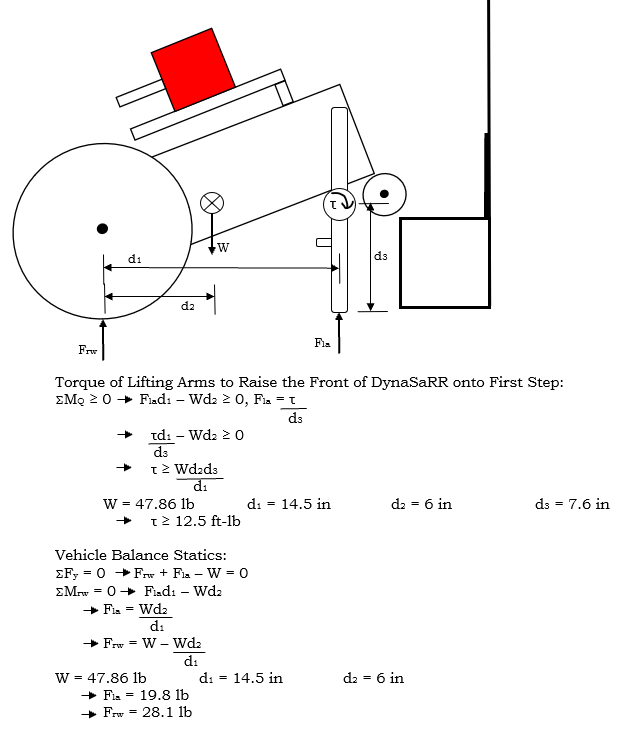
\includegraphics[width=0.9\textwidth]{Images/analysis3_wall1.png}
    \caption{Free Body Diagram and Calculations for DynaSaRR to Traverse Wall- Stage 1}
    \label{fig:analysis3_wall1}
\end{figure}
\vfill
\newpage

\label{fig:analysis4_wall2}
\begin{figure}[hp]
    \centering
    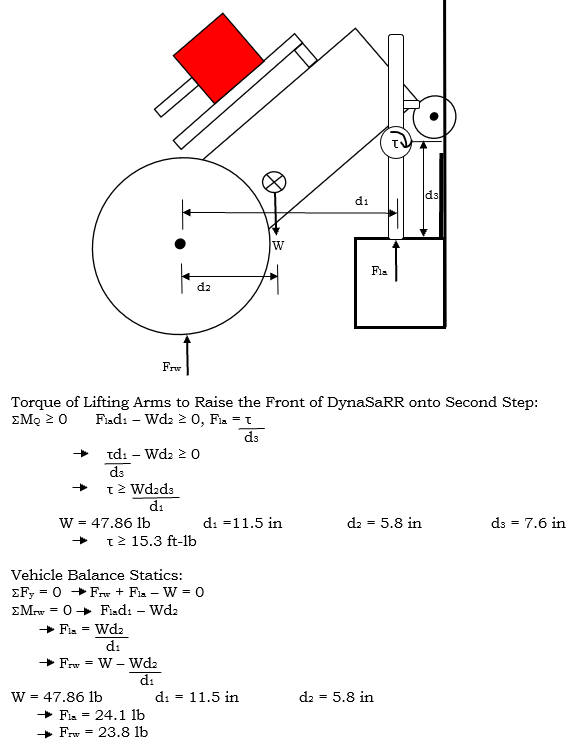
\includegraphics[width=0.7\textwidth]{Images/analysis4_wall2.png}
    \caption{Free Body Diagram and Calculations for DynaSaRR to Traverse Wall- Stage 2}
    \label{fig:analysis4_wall2}
\end{figure}
\vfill
\newpage

\label{fig:analysis5_wall3}
\begin{figure}[hp]
    \centering
    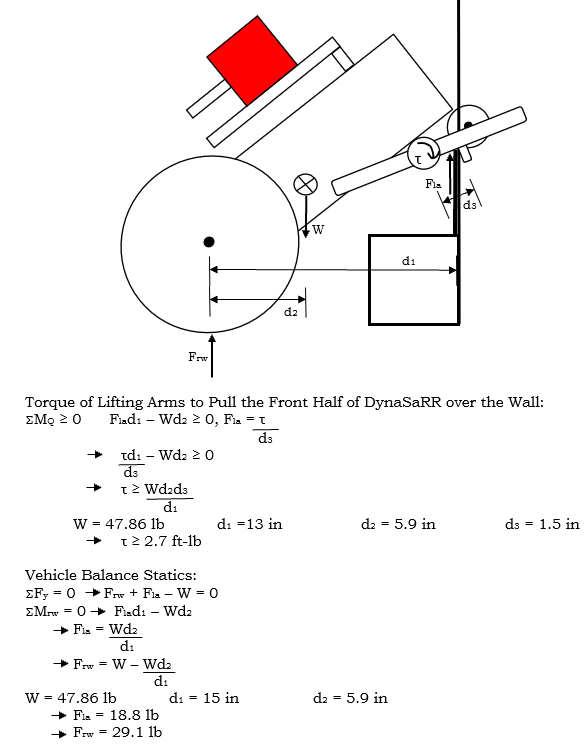
\includegraphics[width=0.7\textwidth]{Images/analysis5_wall3.png}
    \caption{Free Body Diagram and Calculations for DynaSaRR to Traverse Wall- Stage 3}
    \label{fig:analysis5_wall3}
\end{figure}
\vfill
\newpage

Using the the published data, The SaRRchaeologists found that an RPM of 58 was associated with the necessary raw torque of the lifting arm motor, 1.3 newton-meters. Using the 24:1 gearing ratio again and equation (3),

\begin{equation}
    RPM_{new} = \frac{RPM_{original}}{gearRatio} 
\end{equation}


it was calculated that the RPM of the lifting arm would be approximately 4. As such, it would take approximately 22.5 seconds for the lifting arm to rotate 270 \degrees, the estimate required to get it over the wall. However, in practice, the lifting arms were found to rotate faster than this, as the wall traversal took a significantly shorter time (see section 5.1).

To get over the highest point of the wall, the configuration shown below in Figure \ref{fig:analysis6_wall4} illustrated that as long as DynaSaRR's center of mass was to the right of the pivot point, p, DynaSaRR would tip over the wall. 
\begin{equation}
    \sum M_{p} = -W*d<0
\end{equation}
\label{fig:analysis6_wall4}
\begin{figure}[hb]
    \centering
    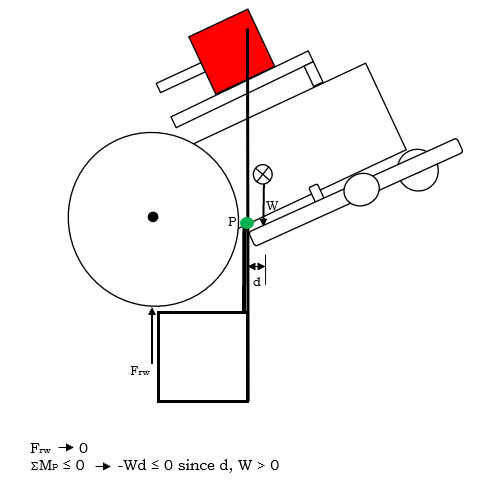
\includegraphics[width=0.6\linewidth]{Images/analysis6_wall4.png}
    \caption{Free Body Diagram and Calculations for DynaSaRR to Traverse Wall- Stage 4}
    \label{fig:analysis6_wall4}
\end{figure}
\vfill
\newpage

When examining static-stability margins, Figure \ref{fig:analysis6_wall4} provides a good demonstration of DynaSaRR's ability to tip over the wall. In this configuration, the center of mass was approximately 0.5 in. in front of the pivot point. This implied that DynaSaRR had just enough weight in front of this point for the front end to fall down, since the distance between the pivot point and the center of mass only had to be greater than zero. Since this measured distance was fairly small, it did not guarantee that the robot would tip over fully on its on, so the lifting arms acted as a secondary tool for the SaRR to traverse the highest point of the wall. The lifting arms pushed against the back of the wall to ensure that the center of mass shifted in front of the pivot point. If the center of mass was shifted further forward, it would be easier for DynaSaRR to tip over the wall. One way this could be achieved would be to shorten the length of the medkit arm. However, the SaRRchaeologists determined that a longer medkit arm was needed in order to deposit the medkit into the basket accurately. While this made completing the final task of the obstacle course easier, it decreased the margin of error during wall traversal. If the center of mass was shifted back by anything greater than 0.5 in., these calculations showed DynaSaRR would not be able to tip over the wall.

The final free body diagram of the wall traversal calculated the force on the front wheels upon dismounting hte walls. The SaRRchaeologists knew that the front wheels would be feel a much greater force compared to their normal driving configuration, since they would be the first part of DynaSaRR to make contact with the ground. Therefore, shocks were added to the front wheels, which were mounted to the chassis with steel forks at a 45\degree angle. The angle allowed for them to be further out from the front of the chassis. This was intended to prevent the front of the chassis from making contact with the ground during any failed trials while testing by stopping the robot's fall earlier. It was found in Figure \ref{fig:analysis7_wall5} that the front wheels experienced a force of 25.8 lbf. Initially, the SaRRchaeologists thought that the front wheels would feel the entire force of DynaSaRR's weight. However, after watching multiple videos of DynaSaRR traversing the wall and creating different free body diagram configurations, it was noted that the back wheels remained in contact with the wall when the front wheels first made contact with the ground. Therefore, the front wheels experienced less force than previously expected, but the shocks remained useful in preventing the sudden impact from damaging more sensitive parts of the assembly.

\label{fig:analysis7_wall5}
\begin{figure}[hb]
    \centering
    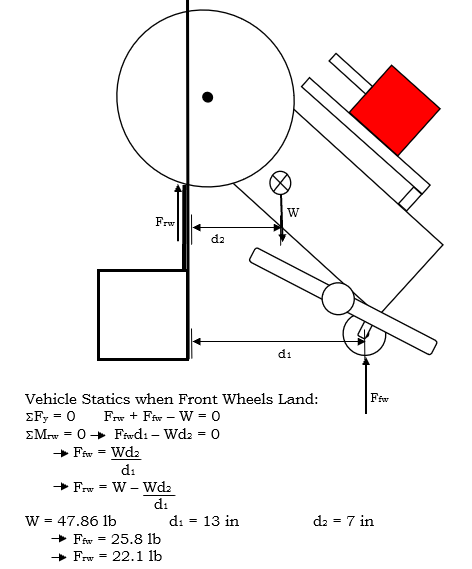
\includegraphics[width=0.7\linewidth]{Images/analysis7_wall5.png}
    \caption{Free Body Diagram and Calculations for DynaSaRR to Traverse Wall- Stage 5}
    \label{fig:analysis7_wall5}
\end{figure}
\vfill
\newpage
\clearpage

\subsection{Control Algorithm}
1- Block Diagrams

In open-loop mode, each of the robot's functions is assigned to a lever on the controller. The value outputted by the controller is proportionally mapped to the range of each motor driver, which then sends the appropriate signal to the motor to complete the action.


Once switched into autonomous mode, DynaSaRR first checks if the wall has been cleared. This condition can be triggered by either a) completing the wallTraverse function, or b) being manually marked as completed using the left switch on the remote. If it is still marked as false, it goes into the wallTraverse function, which gives 25 \percent forward power to the rear wheels and 75 \percent forward power to the lifting arms until the robot has climbed the two steps and has its front wheels hooked over the top of the wall. It then gives full forward power to the wheels and lifting arms in order to pull the robot over the wall. Having completed this part of the course, and with the wall marked as cleared, DynaSaRR goes into chute traversal mode. It reads the difference between the two proximity sensors placed on either side of the front of the frame, and turns slightly away from whichever wall is closer. Between readings, it drives slightly forward to ensure that it does not get stuck oscillating back and forth between the walls without making progress. Upon exiting the chute, light tracking is activated, with the code reading the difference in brightness between the two light sensors mounted on the front crossbar and pointed inward so that each one's field of view overlaps the other's. The algorithm turns the robot to the side with the dimmer reading (i.e., if the left light sensor, which points slightly right across the front of the robot, reads a brighter value, the robot will turn slightly to the right to re-enter the column of light) and drives forward when both sensors read approximately equal values, i.e., when the robot is facing directly into the light. Should DynaSaRR turn too far out of the light column and the light signal drop too low, it begins to rotate slowly to the right until it is able to reacquire the signal. Finally, once the proximity sensor mounted to the front of the frame detects the presence of the medkit deposit basket, the robot stops driving and brings the medkit arm forward to place the medkit in the basket.
\section{Specifications}
\subsection{Size, Weight, Speed}
Below is a list of design specifications for DynaSaRR. Drive wheels with a 12 inch diameter were selected, with inflatable rubber tires for enhanced control while navigating and increased traction during wall traversal. This design choice was intended to reduce slippage and ensure that more torque from the motor would be used to power the wheels than if tires with less traction were used, thereby increasing speed on the ground and obstacle traversing ability. DynaSaRR's chassis was designed to be longer than that of the sample robot in order to accommodate the lifting arm mechanism which would propel it over the wall.

The frame was constructed from T-slotted 80/20 aluminum 6061 extrusions. Two levels of rectangular frame were separated by 3-inch pieces of extrusion, creating two levels onto which parts could be mounted. This shape allowed for maximum organizational efficiency, easy mounting of parts, and modularity, while maintaining a compact, maneuverable chassis.

Based on the initial CAD model, in which a weight estimate was calculated in CREO 5.0 using material assignment and inputting calculated densities of the parts already possessed by the team, including the drill batteries, Teensy board, and various motors, DynaSaRR was specified to weigh 45 lbs. The true weight, measured after the robot was manufactured and assembled, came to 44.3 lbs--very close to the estimated weight. This allowed for precise values to be in the calculations, as the weight of any component or subsystem calculated in CREO could be assumed to be very close to its real weight.


\begin{itemize}
    \item Total Weight: 44.3 lbs
    \item Frame Width: 12 in
    \item Frame Length: 19.5 in
    \item Frame Height: 5 in
    \item Chassis Clearance Height: 3.9 in
    \item Drive Wheel Diameter: 12 in
    \item Drive Wheel Width: 1.7 in
    \item Max SaRR Width: 15 in
    \item Max SaRR Length (Lifting Arms Up): 22 in
    \item Total SaRR Height: 14 in
\end{itemize}

In order to estimate DynaSaRR's speed along a flat surface, it was first necessary to calculate the total force required to maintain speed:
$$F_{tot} = F_r + F_{drag}.$$
$F_r$ is the rolling resistance, and is calculated as $$F_r = c*W,$$ where $c$ is the rolling resistance coefficient of the tires, and $W = m*g$ is the weight of the robot (mass times acceleration due to gravity). $c$ for bike tires on waxed wood was found to be $0.002$, and on asphalt was $0.005$. From these values, $c$ for our tires on linoleum was estimated be $0.004$. The weight of DynaSaRR was 48 lbs. with the med kit, so $F_r$ was calculated as $77.23\frac{lb*in}{s^2}$.
$$ F_{drag} = \frac{C_d*A* \rho_{air}*V^2}{2}.$$
Here, $C_d$ is the coefficient of drag, which was estimated to be 1.16 due to the ratio of length (20in) to height (12in) of approximately 2 of the robot face (calculated for a flat rectangular plate). $A$, the area of the robot, was calculated as $0.3*20*12$, because the SaRRchaeologists estimated that only about $30 \%$ of the 20 by 12 rectangle actually contained material. $\rho_{air} = 4.06*10^-5 \frac{lb}{in^3}$, and $V$ is the velocity of the robot. In order to complete the calculations, the velocity had to be estimated and then the following calculations had to be iterated over until the estimated and calculated velocities matched (detailed calculations are shown in the Appendix). In the final iteration, a velocity of 7mph was assumed, so $F_{drag}$ was calculated as $25.763 \frac{lb*in}{s^2}$. Thus, $F_{tot} = 102.97 \frac{lb*in}{s^2}$. From this, torque was calculated as 
$$ \tau = r_{wheel}*F_{tot}*sin( \theta).$$
Since this calculation was for a flat surface, $\theta = 90 \degree $, and the wheels had a radius of 6 in. Drive train efficiency was estimated to be $84.1 \%$, so actual torque for each of the two driven wheels was calculated as
$$ \tau_{real} = \frac{\tau}{2*0.841} = 367.33 \frac{lb*in^2}{s^2}.$$
This was then multiplied by a safety factor of 2 and converted to Newton-meters, resulting in a torque of $0.22 N*m$. The corresponding RPM (read off Fig. \ref{fig:motorcurve}) at that torque was 4700 rpm, which was converted to a speed by multiplying by the wheel circumference, resulting in a speed estimate of 6.99mph--extremely close to the original estimate. This showed that this iteration of calculations would be an accurate predictor of DynaSaRR's performance: it could be expected to travel at approximately 7mph.

\begin{figure}[ht]
    \centering
    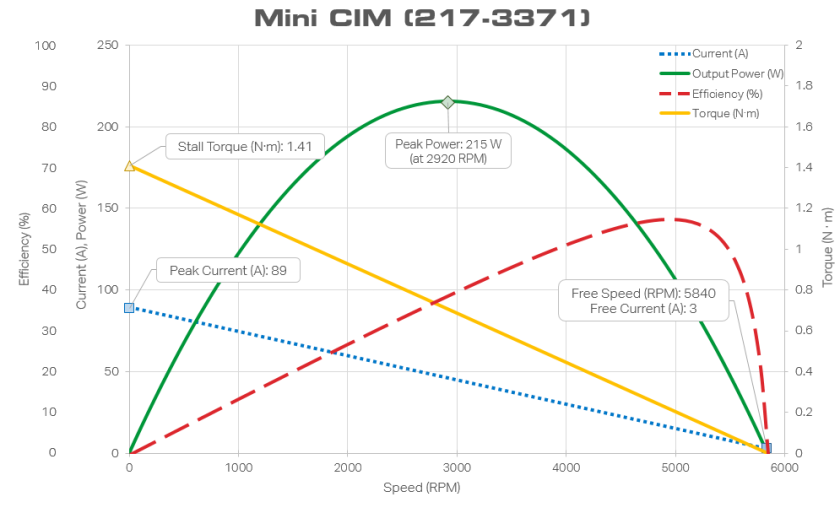
\includegraphics[width=\textwidth]{mini-cim-motor-curve}
    \caption{Motor Curves for the VEX Motors}
    \label{fig:motorcurve}
\end{figure}

DynaSaRR had an estimated top speed of 7.2 mph or 10.56 feet per second. Additionally, the turning radius was calculated to be 19.6 in. As such, moving at top speed, it would take the DynaSaRR approximately 10 seconds to complete the entire course (approximately 100 ft), with the exception of the wall traversal portion. However, this is clearly not a realistic expectation, as the robot would only be moving at top speed for approximately the first 50 feet of the course after picking up the medkit. Based on open- and closed-loop tests, the SaRRchaeologists estimated that it would take DynaSarr approximately 10 seconds to retrieve the medkit, 10 seconds to circumvent the pylon (in addition to the approximately 5 seconds of top-speed driving), 10 seconds to breach the wall, 30 seconds for chute traversal, and 45 seconds for light tracking and medkit placement. Combining these times, the SaRRchaeologists predict that it will take approximately 2 minutes to complete the course

The maximum communication range of the remote control system used was right around 250 ft in ideal testing conditions (a linear, enclosed section of hallway). The SaRR ran through autonomous tasks at any distance from the remote controller. The range of the remote controller batteries was no more than 6 hours of continuous usage. The range till failure of the drill batteries that provided the primary power to the SaRR was about 210 minutes of intermittent task testing (chute navigation, light navigation, wall traversal). However, performance was limited significantly after only 30-45 minutes of intermittent testing. 



\subsection{Operational and Navigational Modes}
The SaRR had two modes of control: open-loop mode, in which it was controlled by inputs to the controller, and autonomous mode, in which it was operated by closed-loop Arduino code sent to a Teensy board. The open-loop navigation was used to locate and retrieve the medkit, then move to the front of the wall obstacle, while the rest of the course was navigated autonomously.

In order to successfully navigate to the medkit, pick it up, and then drive to the front of the wall obstacle, the open-loop remote controller (the human-technology interface in this design) had 4 directional inputs programmed to the right joystick: forward, backward, right turn and left turn. Moving the left joystick vertically triggered the lifting and lowering of the medkit retrieval arm, and horizontal motion controlled the rotation of the lifting arms. The controller also had 2 switches which amplified an isolated channel based on the location of the corresponding knob located on the controller. The right switch triggered autonomous mode. The left switch triggered a reset of several booleans--these could be changed in the code in order to have autonomous mode go directly to a certain function (e.g., skip over the wallTraverse() function and go directly to chuteTraverse()). The signals from the remote controller were obtained on the SaRR by a wireless receiver and were read into the Teensy micro-controller, where actions were assigned based on the values transmitted. In open-loop mode, these were the only inputs received by the SaRR.

When the right shoulder switch was flipped, the value of the designated channel breached a specified input threshold, activating autonomous mode. In autonomous mode, the only inputs to the micro-controller came from three proximity sensors and two light sensors. One proximity sensor was located on the front of the SaRR, and the other two were located on opposite sides of the frame. The two light sensors were located on the top of the bottom beam of the frame and were facing forward. 

When in autonomous mode, the SaRR had to complete four tasks: traverse the wall, navigate the chute, find and track the light source, and drop the medkit into the basket. 

The wall traversal was completed by the two lifting arms on either side of the frame. These arms rotated on an axle and were connected to a third motor with output torque ~1.3 Nm. They had a pre-programmed sequence that first rotated forward 180 \degree, an action completed accurately (to within ~5\degree on full charge) using the speed of the motor at a specified power and a timed action in the code sequence. While the arms rotated, the Teensy drove the rear wheels forward. The lifting arms then rotated around once again, pushing off the top of the step and lifting the front wheels over the top of the wall as the rear wheels drove forward. A third rotation was then completed, latching onto the top of the wall and, with the assistance of the large driving wheels in the rear, levering and pulling the SaRR over the obstacle. The lifting arm rotation sequence was written into the code and was adjusted for accuracy and timing in trials. As soon as the lifting arms were through their final rotation and the SaRR was on the other side of the wall, autonomous chute navigation was engaged in the Teensy code.

The SaRR then moved forward and began to navigate the chute. This was done through the use of the proximity sensors on the front, left and right of the frame, providing feedback that was used to issue instructions to the SaRR that kept it well within the walls of the chute. Upon approaching a wall, the algorithm imitated a proportional controller, turning away from the closest wall until the difference in proximity sensors was equalized. Success was achieved after testing and tuning.

Once through the chute, the SaRR no longer registered a high value from the proximity sensors residing on the side of the frame and entered light tracking mode. In this mode, the SaRR rotated clockwise until the forward-facing light sensors detected the drop zone flashlight. At this point, the robot moved forward, continuously monitoring the strength of the light to ensure it was moving in the right direction and turning back into the column of light. This action was implemented with similar code that checked the values of the light sensors and adjusted the robot's position to minimize the difference between them. Once the front-mounted proximity sensor registered that the SaRR was close to the drop zone, the code stopped the robot and lowered the medkit arm, dropping it into the basket.
\section{Creo Rendering and Drawings of Important Sub-Assemblies}

\begin{figure}[ht]
    \centering
    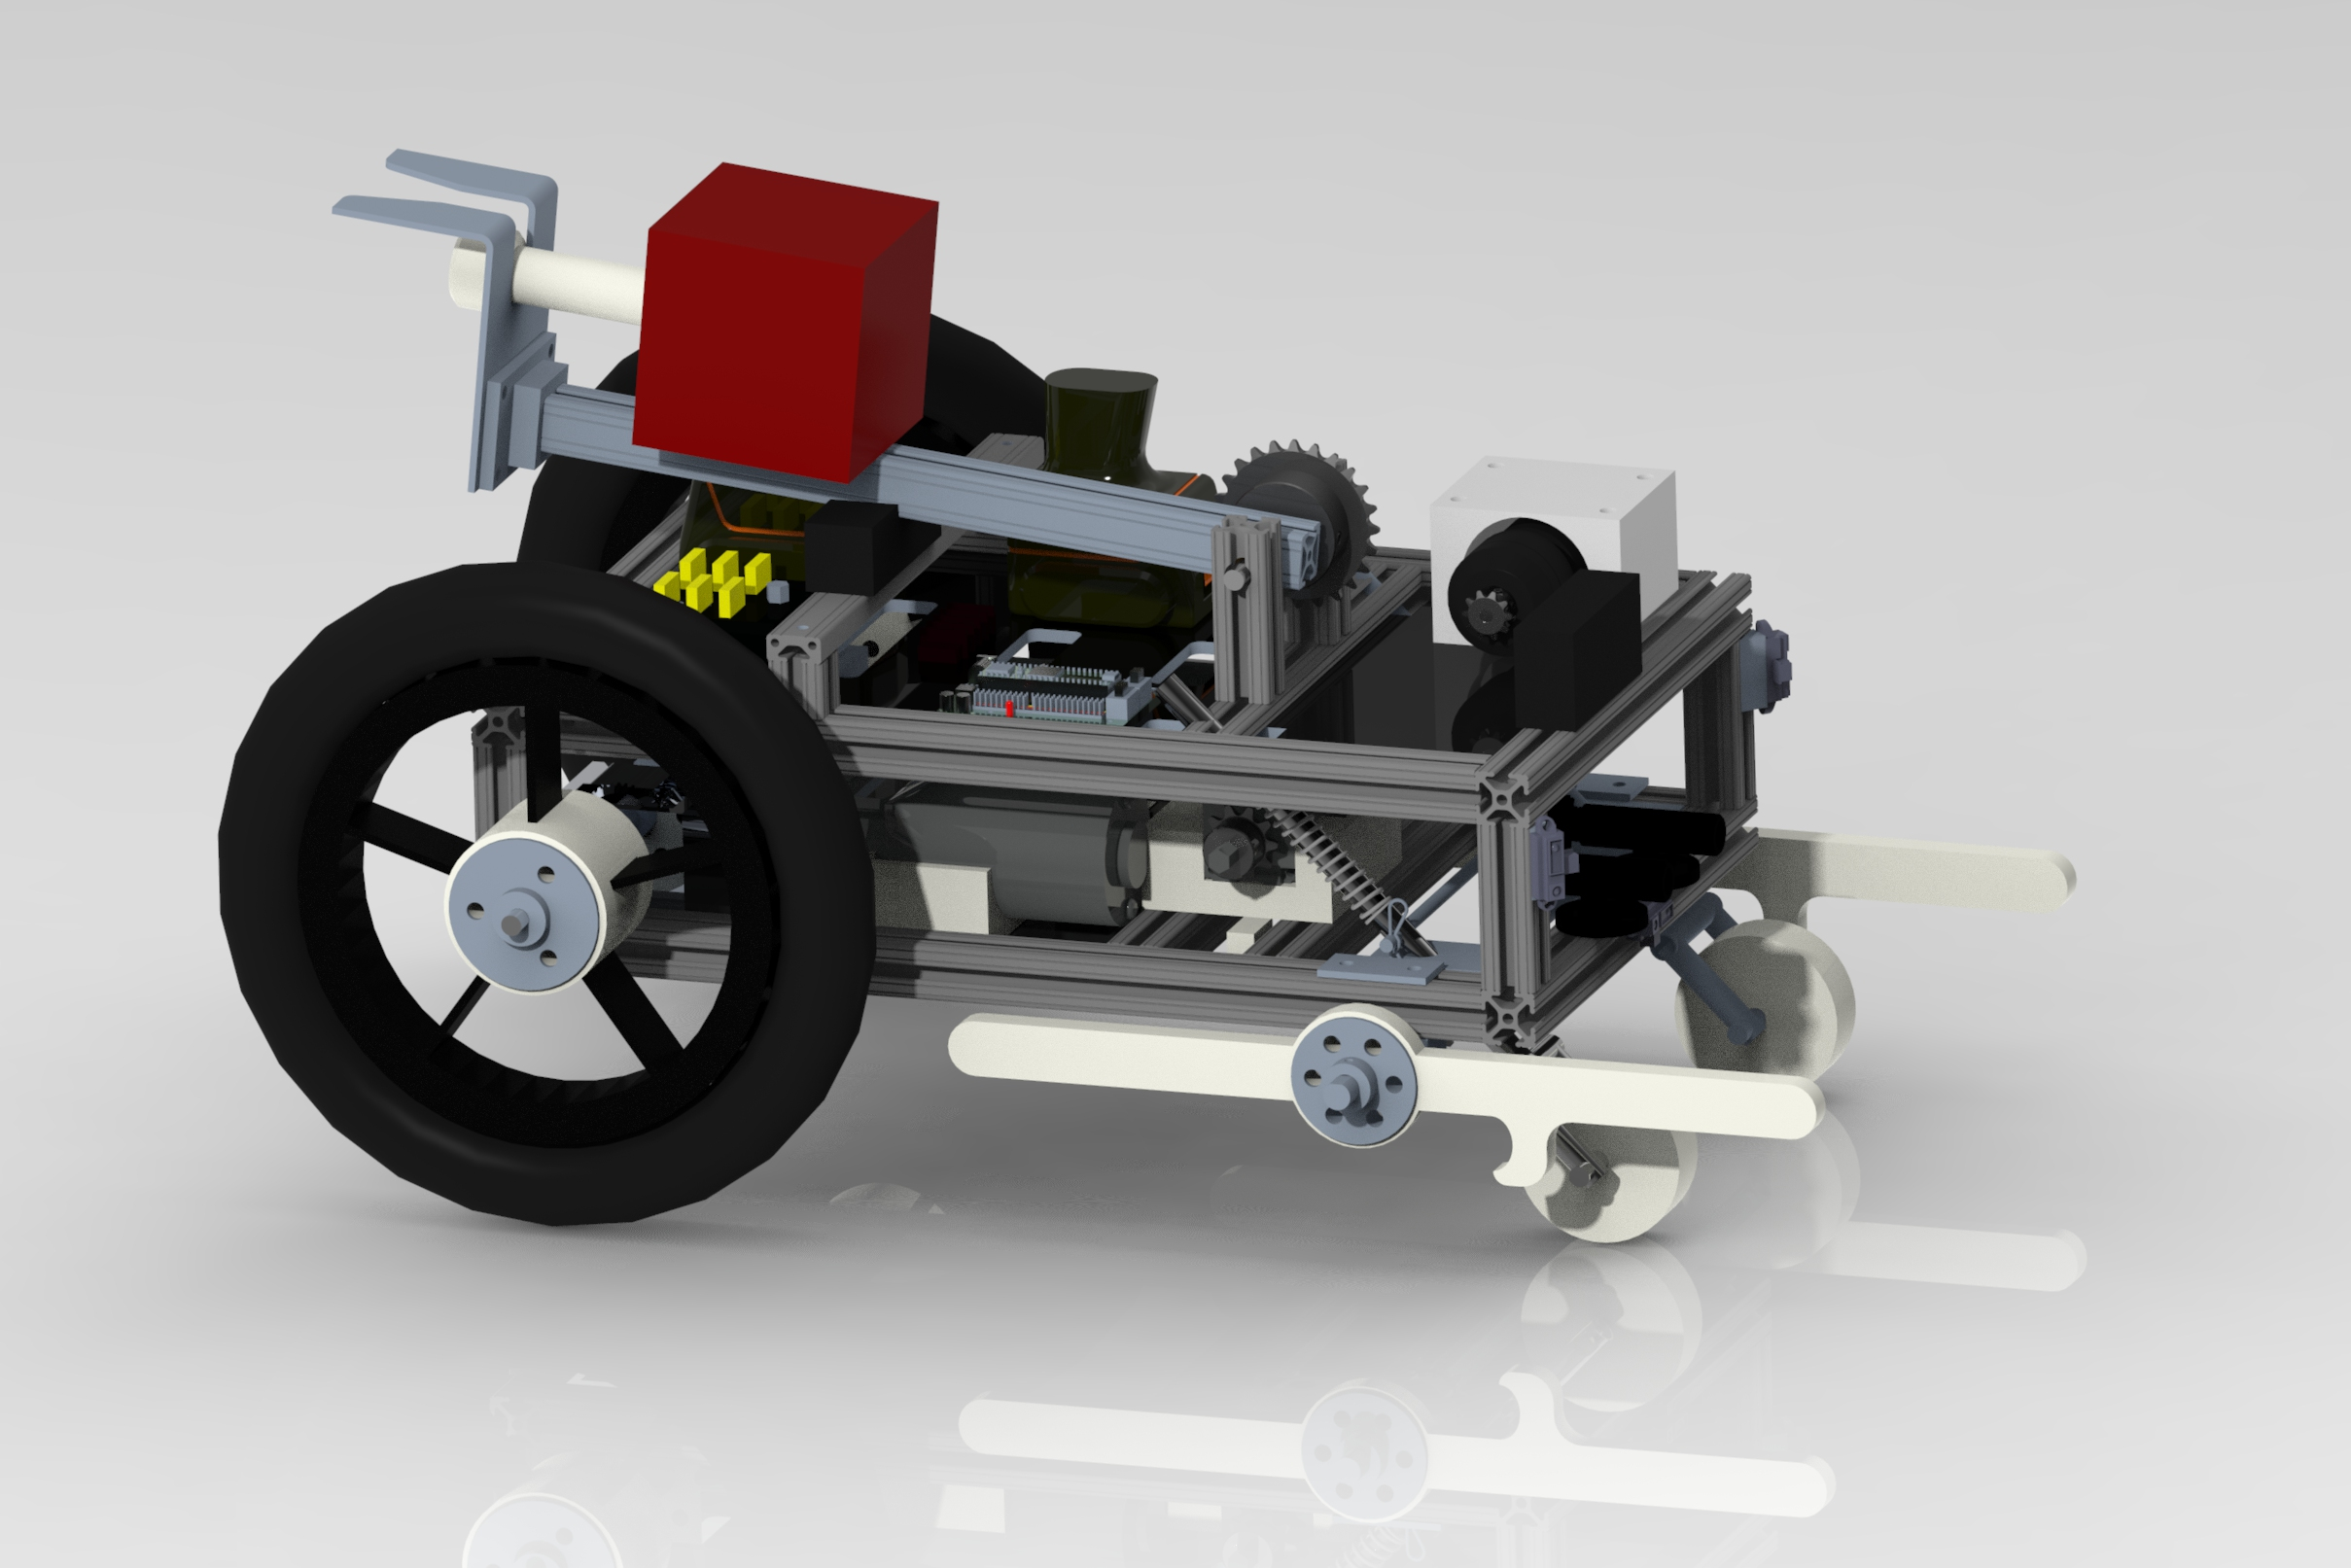
\includegraphics[width=0.7\columnwidth]{./Images/FDR_pretty_picture_2}
    \caption{Final rendering of DynaSaRR}
\end{figure}

\begin{landscape}
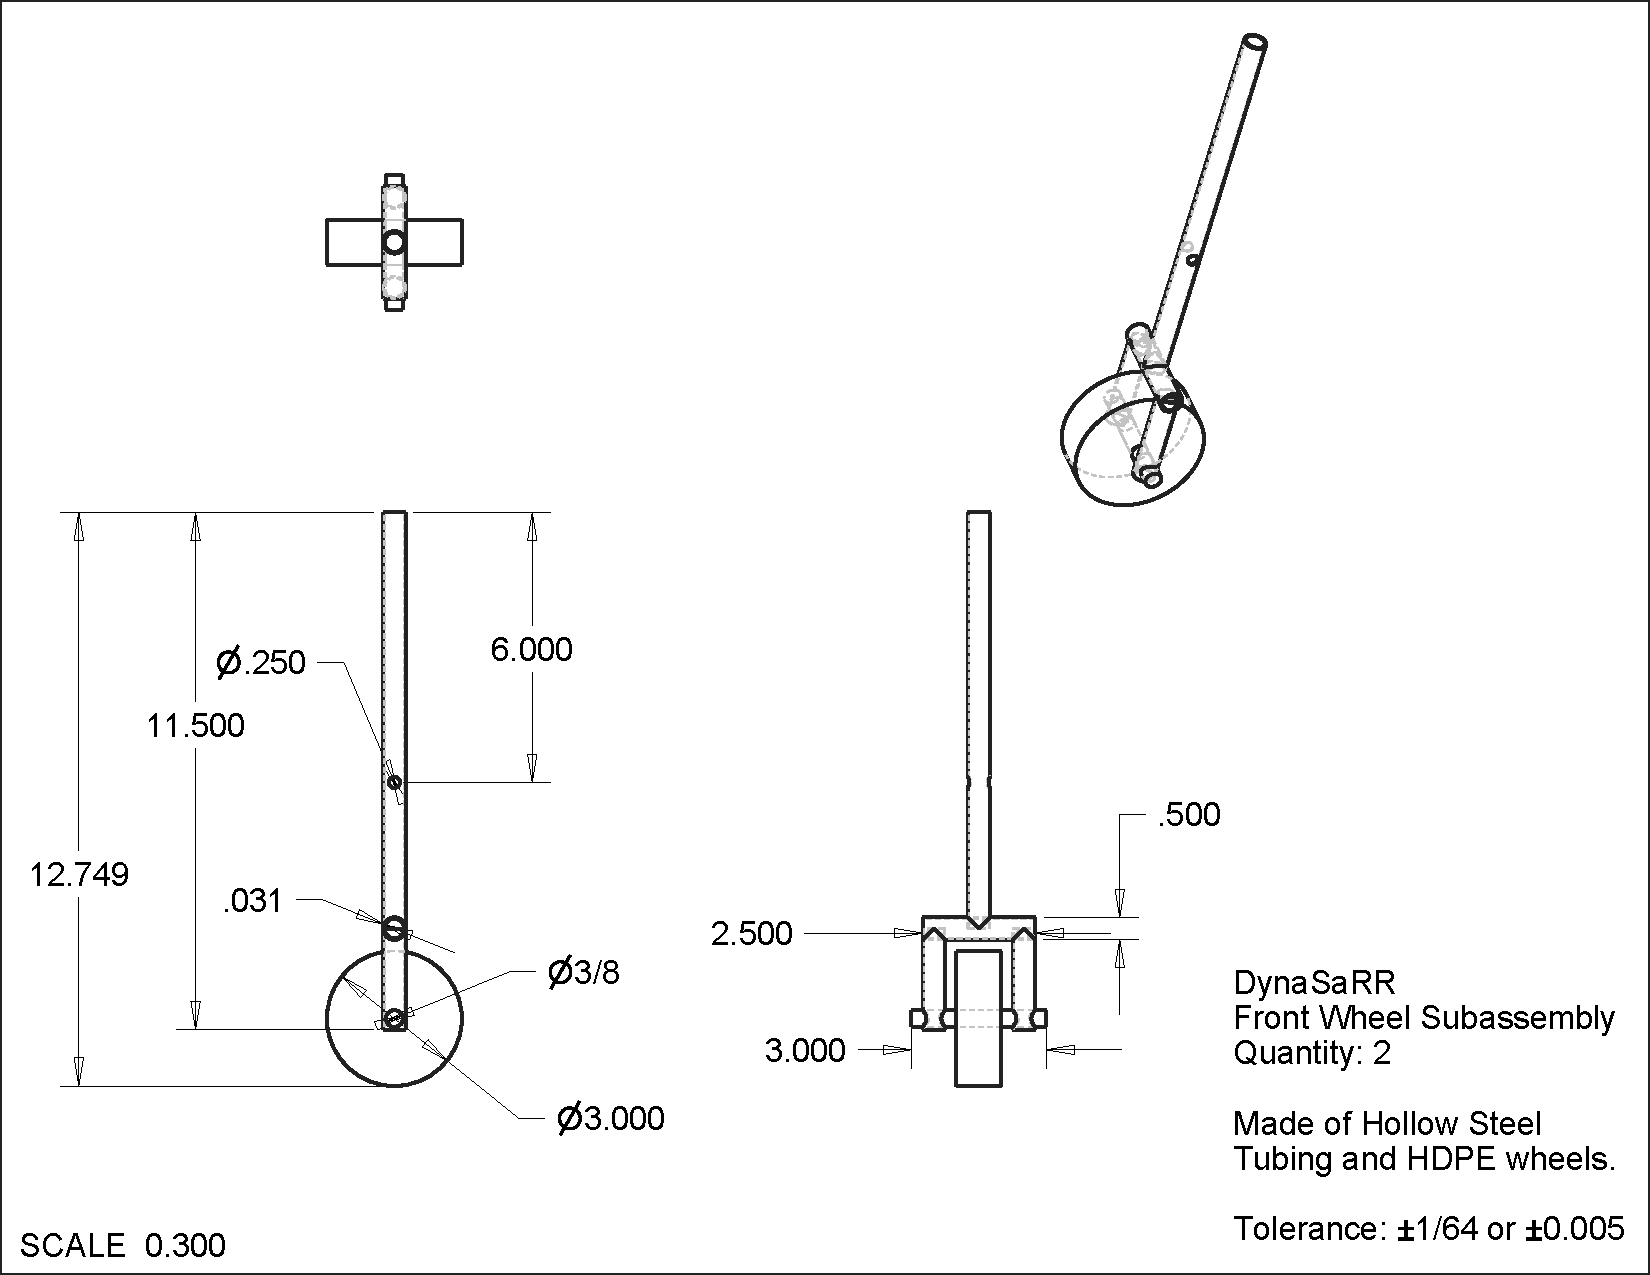
\includepdf[pages={-},angle=90]{./drawings/front_wheel_subassembly}
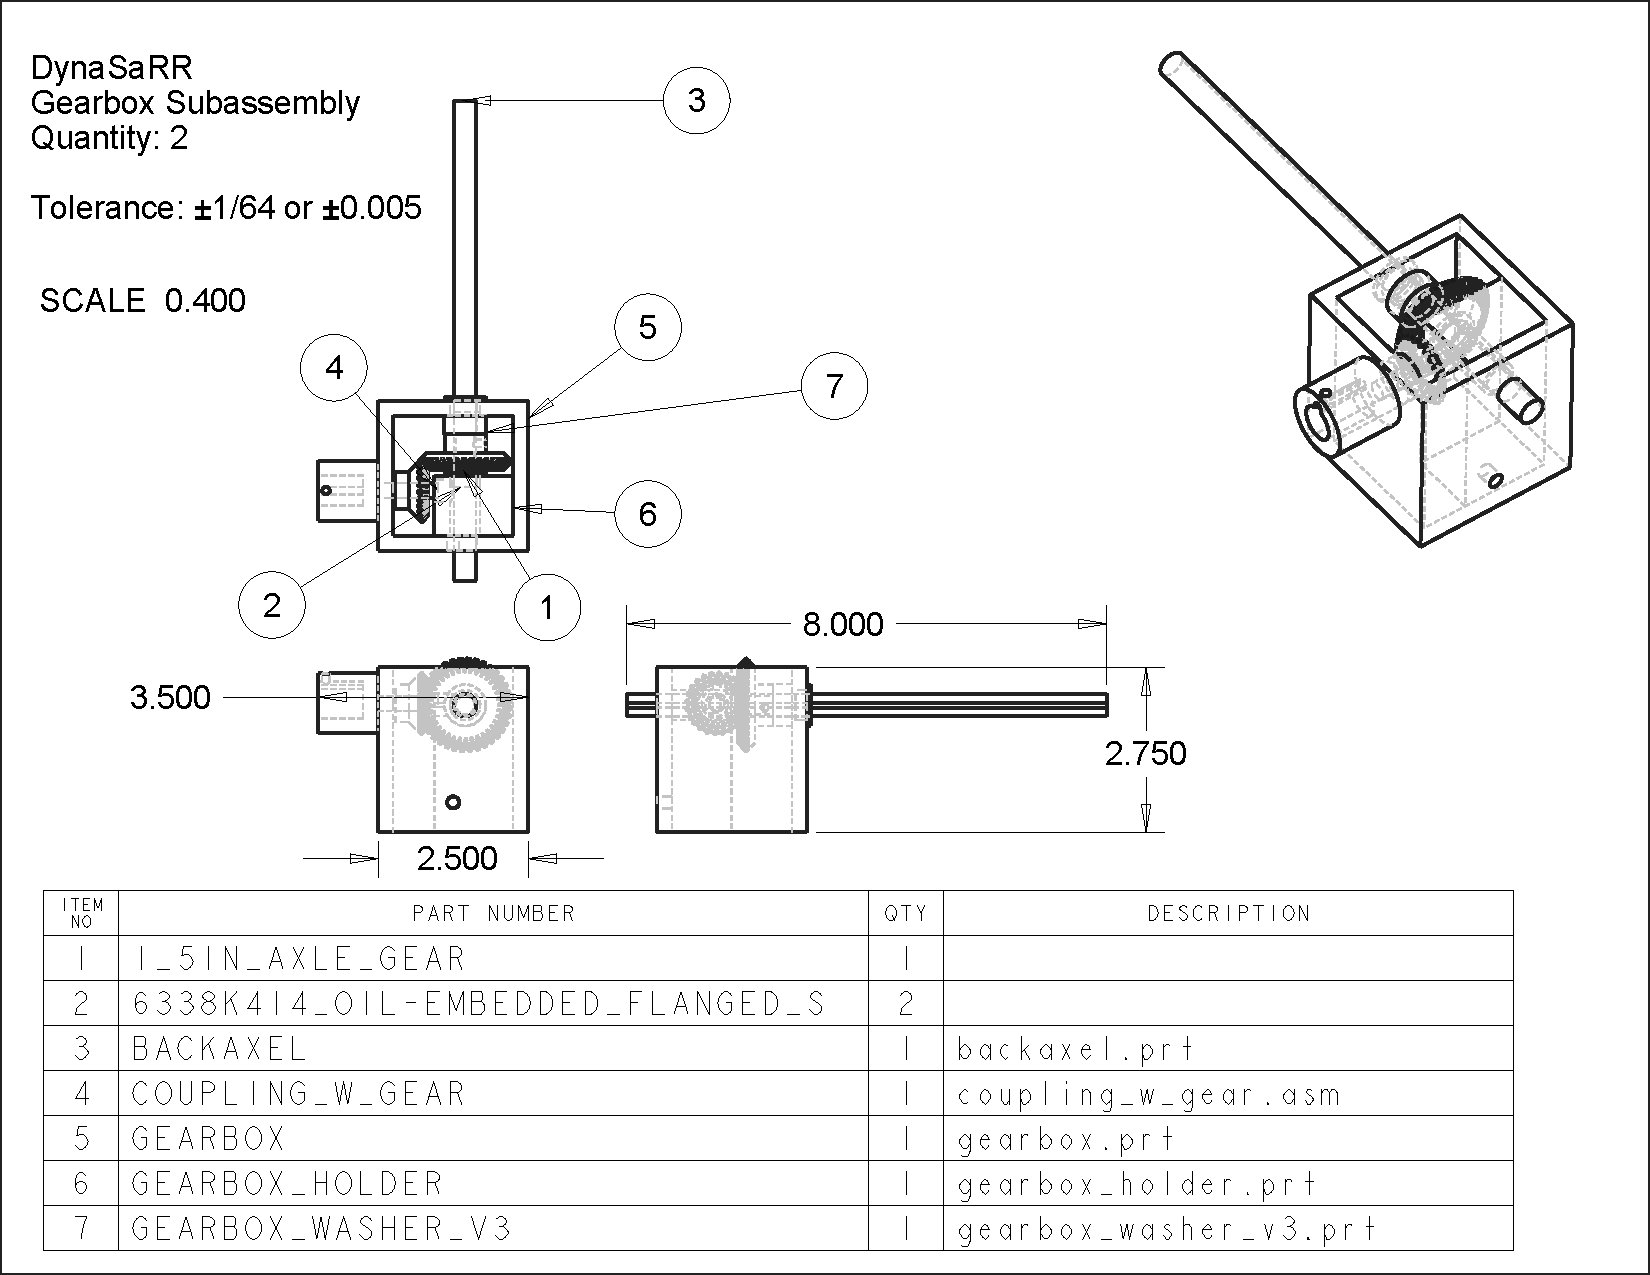
\includepdf[pages={-},angle=90]{./drawings/gearbox_subassembly_drawing}
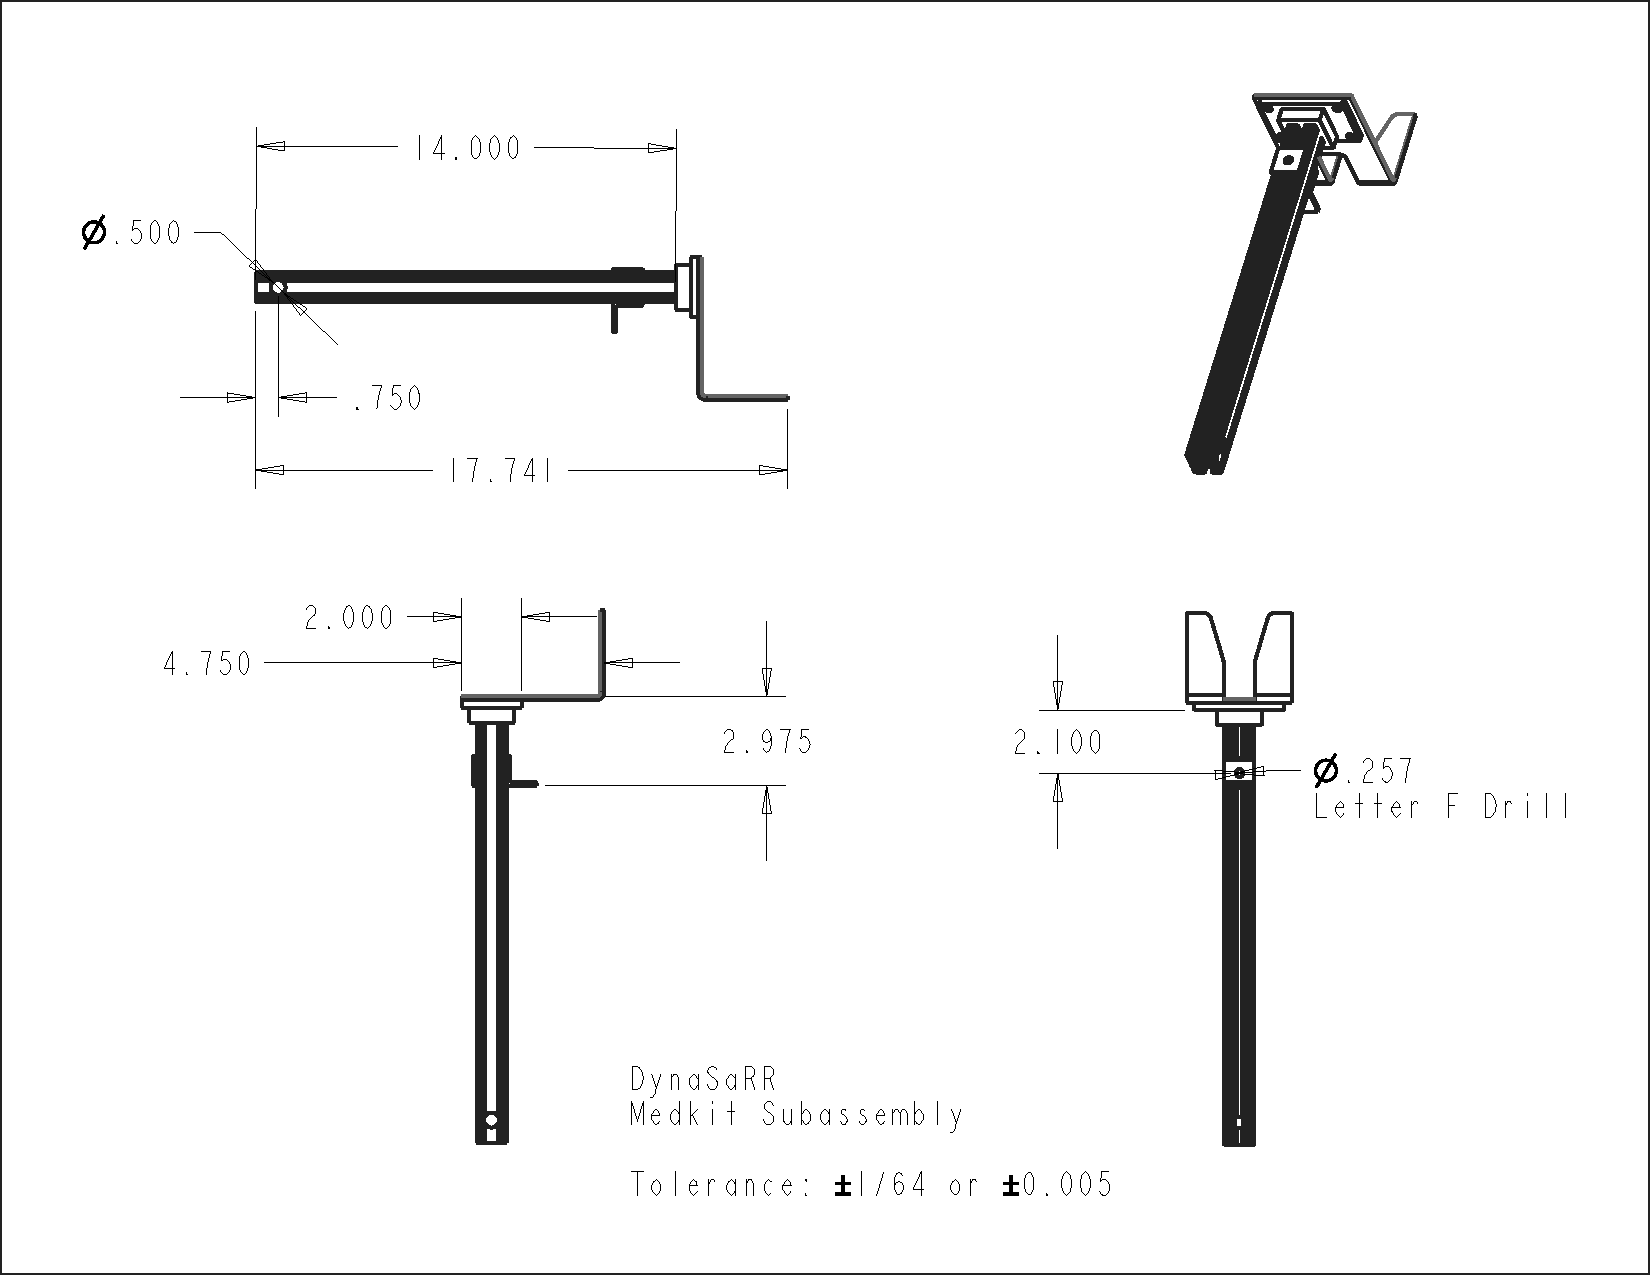
\includepdf[pages={-},angle=90]{./drawings/medkit_subassembly_v2}
\end{landscape}
 \section{Test Results}
 
Preliminary Testing: Autonomous operations were performed in three steps, beginning with code written for the light source detection procedure. Coding the light detection algorithm meant reading values from both light sensors mounted about 2 inches apart on the front of the chassis and pointed slightly inward so their fields of vision overlapped, and adjusting course direction based on the differences in readings. To first detect the light, DynaSaRR first rotated slowly clockwise until a signal above the threshold was acquired. This was intended to make the SaRR better suited to real-world performace, as it would need to detect the light source regardless of its position. Under these test conditions, however, the light source was placed to the right the chute exit. Thus, once DynaSaRR recognized it had exited the chute using the side-facing proximity sensors, it began to turn clockwise in search of the light source. Once the robot acquired the light signal and determined that it was facing directly into the light (the two light sensors read approximately the same value), it began to drive forward towards the basket. This command continued until the value read by one light sensor differed significantly from the other. Once this difference was been detected, the robot adjusted it course by turning slightly towards the dimmer light sensor until the values read were similar again. This process repeated until DynaSaRR's front-mounted proximity sensor detected the delivery basket, and notified DynaSaRR to stop within approximately 6" of the bin. At that point, the medkit motor arm was is activated and the medkit was dropped into the bin. Having completed its delivery, the robot paused and then backed up several inches, releasing the medkit fully. Programming this operation presented several challenges, particularly with the variation in results while testing. It took several runs to determine how much voltage should be sent to each motor in order for turns to be made consistently. Too little, and the robot wouldn't turn, but too much and the robot would overshoot the column of light and oscillate back and forth trying to realign itself. The key turned out to be a medium voltage for a short duration of time. This enabled the bot to turn consistently but with only minor adjustments to direction. Unfortunately, the robot's performance was not consistent over time, as the draining batteries resulted in the same amount of voltage to the motor producing a much smaller turn, so the code was designed to run successfully at close to full battery charge. The final step of the code also required tuning, because it required DynaSaRR to stop at the same distance (within 1 inch) every time. The robot needed to be both perfectly aligned and perfectly distanced from the wall for the medkit arm to successfully drop off the medkit. This meant slowly fine tuning the threshold value for the front proximity sensor. From a test distance of 30 feet, it took DynaSaRR an average of 29 seconds to deliver the medkit in testing.

The next challenge, also noted by a milestone, was autonomous navigation of the chute. Coding this portion was not as difficult as the deposition step once the turn command was tested extensively in the first coding portion. After breaching the wall, DynaSaRR would enter the chute. Chute detection began when both side-mounted proximity sensors registered sharp change in distance. Once the robot entered the chute, it slowed slightly and rapidly updated its readings for both proximity sensors. As it approached a corner or turn, the difference between to the two sensors triggered it to turn away from the closer wall until the sensors began reading similar numbers again. Interestingly, the sensors were originally mounted at about a 45 degree angle facing forward in order to preemptively detect turns and adjust before reaching them. However, the algorithm worked much more consistently when keeping the sensors facing fully sideways, perpendicular to the direction of driving. Once the sensors were mounted this way, DynaSaRR successfully navigated the chute on its first test run, and the results were found to be repeatable until battery drainage caused the course adjustments to fail. On test day, chute navigation took approximately 25 seconds. 

Last, but certainly not least, was the autonomous wall traversal. This operation proved especially difficult because it required precise timing of both the driving wheels and lifting arms to propel the rather heavy robot over the wall. Open-loop wall breaching was immediately and consistently successful without the addition of the medkit arm retrieval mechanism or the medkit itself. However, the additional weight of the medkit and arm shifted the center of gravity backward, making open-loop navigation over the wall less consistent. After adding bolts to the lifting arms, open-loop traversal became reliable again. 

When testing autonomous wall breaching, the SaRRchaeologists found that it was important to keep both batteries fresh, and to periodically tighten the lifting arm set screws. Repeated attempts--both successes and failures--put a lot of stress on the chassis, even with the shock-absorbing springs on the front wheels, but no major damage was sustained despite several inversions and hard landings. To trigger the three-step wall breaching code, the front proximity sensor first detected that the robot was within a few inches of the first step. Then, the lifting arms rotated to lift the front wheels off the ground and, with the back wheels driving, placed the front wheels atop the first step. This command was repeated to prop the robot up onto the top of the wall. During testing, pauses were inserted in between each separate motion to ensure breaching the wall was not a function of momentum, which could be inconsistent. With the front wheels over the top of the wall and the back wheels still on the ground, full power was given to the lifting arms and rear wheels to pull the robot over the wall. By tweaking and tuning the code, success was eventually achieved in breaching the wall. However, results were inconsistent: the code would not always work the same way each time, and every few attempts, the robot would end up flipping over completely, either before breaching the wall or after landing. Despite many test runs, no mechanical or structural damage was obtained, which proved that the SaRRchaeologists had achieved their goal of making DynaSaRR thoroughly robust, particularly with respect to vertical drops. In the end, wall breaching took approximately 15 seconds to complete.

On the day of competition, DynaSaRR did not perform as well as expected due to some minor problems with constants in autonomous code, energy inefficiencies, and testing conditions that were slightly different than expected. The light sensing code threshold for the difference between the two sensor readings was slightly too large, making it unlikely that the SaRR would correctly track the light unless conditions of ambient light were nearly ideal and the light sensors in use were perfectly oriented. Along with this error, one of the light sensors in use was showing inconsistent readings the night before and just after testing, making the code unlikely to work as it did previously. In particular, the inconsistent readings resulted in the code believing that the robot was always to the left of the light column and therefore turning to the right to reacquire the signal. However, since the robot was already to the right of the ideal path, this resulted in DynaSaRR losing the light signal completely and beginning to spin in an attempt to reacquire it. Additionally, the SaRR very quickly lost ideal operating power, as the drill batteries in use were fairly drained after only one attempt at the course. This greatly reduced the chance of conquering the autonomous portions on subsequent trials, as the constants in use were designed for a battery at full power. Furthermore, this resulted in a failure to successfully breach the wall: in its first attempt with full power, DynaSaRR breached the wall, but was given too much power and flipped over on the dismount. In subsequent attempts, the power provided to the motor was reduced to avoid flipping, but since the batteries had been partially drained, these adjustments caused the robot to fail to pull itself over the final step of the wall. In further tests, the batteries were so drained that the robot was no longer able to breach the wall, even in open-loop mode. Lastly, the conditions of the lab in which the competition was conducted were not the same as those in which tests were completed throughout the semester, leaving the team to work on fine-tuning code in the last few days before the competition, without being able to test code for long periods of time without triggering reliability issues due to draining batteries. While the team believed most problems had been solved, some issues regarding inconsistencies on the floor and reflections around the room were unavoidable, and the SaRRchaeologists were not ultimately able to overcome these challenges within the time frame of the demonstration.

Overall, the physical capabilities of the robot did not limit the performance on competition day. Instead, the performance was limited primarily by code that may not have been robust enough to adjust to new circumstances, as well as problems caused by the draining batteries. 

\newpage
 

\section{Further Work and Conclusions}

DynaSaRR's base was designed so that it could be adapted to any scenario or obstacle. This particular iteration of DynaSaRR was designed so as to best handle the specific objectives for this course: retrieving a medkit, traversing a wall, navigating a chute, and depositing  the medkit. The SaRRchaeolgists carefully analyzed the objectives in order to create the pieces necessary for DynaSaRR's success. What's more, the SaRRchaeologists sought to create a robot that would be robust enough so as to assuage any fear of breakage either prior to or during the navigation of the course. 

The SaRRchaeologists were, undoubtedly, successful in their attempt to create a sturdy and robust robot. By looking at the high stress subsystems, this robot would buckle only if it were to encounter an addition 150 lbf \ref{fig:buck2}. What's more, the initial drop test before the final testing proved DynaSaRR could handle the shock of a drop. Finally, throughout the building process, DynaSaRR experienced many falls, from many angles, and still was able to withstand the hits with little to no damage. 

The SaRRchaeologists were, however, unsuccessful in their complete navigation of the course. It is important to note, however, that DynaSaRR was more than capable of navigating the course while being driven in open-loop mode. Time and time again, the SaRRchaeologists were able to succeed at each and every objective individually. In this respect, it can be said that the SaRRchaeologists were successful in their hardware manufacturing and their overall design.

Ultimately, the closed loop caveat of this task proved to be the downfall of DynaSaRR and the SaRRchaeologists. In spite of being able to successfully traverse the wall and deposit the medkit countless times using open loop, the code used for the closed loop driving proved insufficient. The lack of robust code could be attributed to many things, but the most salient reason was most likely the SaRRchaeologists' simple inability to spend enough time working on the code in the competition conditions. There were many mechanical issues that consumed enough time that the SaRRchaeologists had to continually push back their testing start times. This shortened the amount of time available to troubleshoot and improve the closed-loop code.

Given more time, the SaRRchaeologists would first attempt to find a means to power DynaSaRR such that it could operate at full power for longer. The diminished battery power caused the SaRRchaeologists to have to cease tests sooner and with greater frequency then desired. Subsequently, the group would spend a significant amount of time troubleshooting the code, but the varying performance depending on battery charge ultimately proved to be insurmountable for the SaRRchaeologists within the given time constraints. 





\backmatter
\section{Appendices}
\subsection{Calculations}
\begin{landscape}
\begin{figure}[ht]
    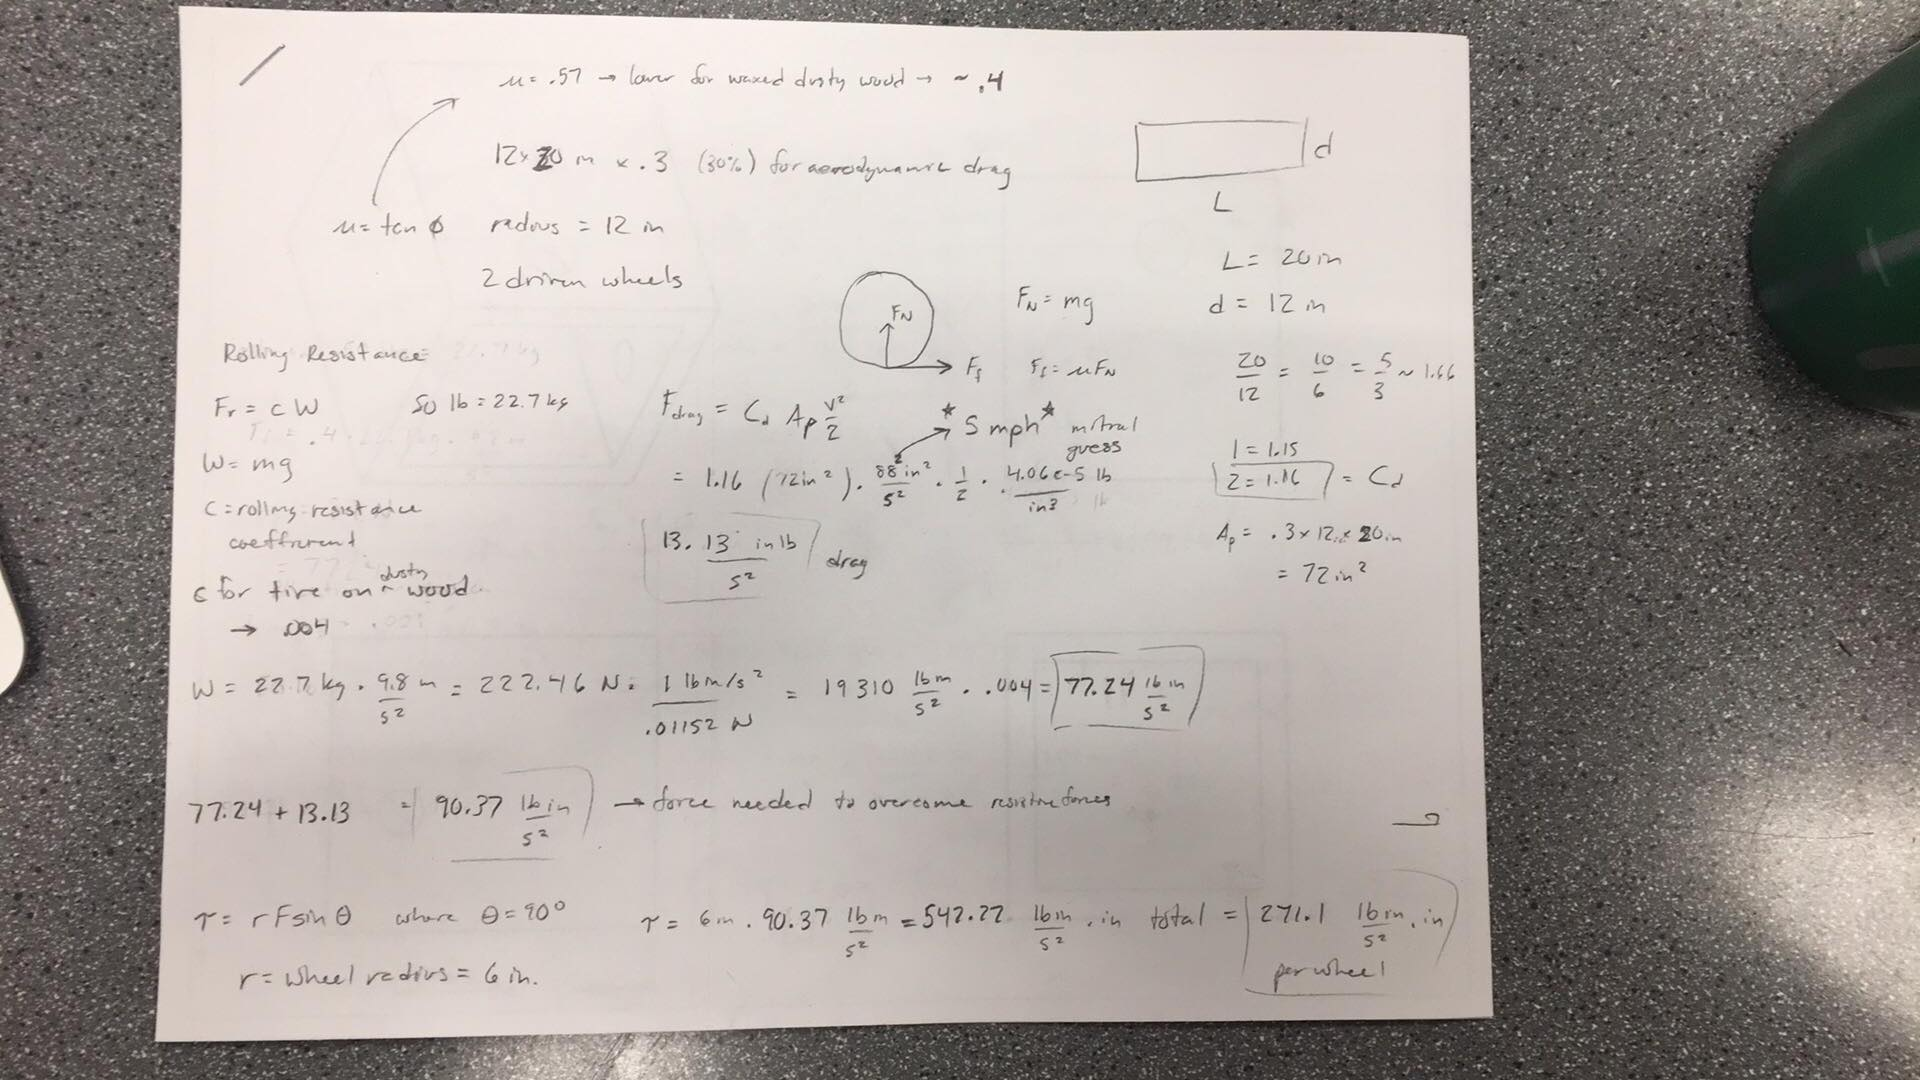
\includegraphics[width=\linewidth]{calculations1}
    \centering
    \caption{Numerical Values and Solutions, Part I}
\end{figure}

\vfill
\newpage

\begin{figure}[ht]
    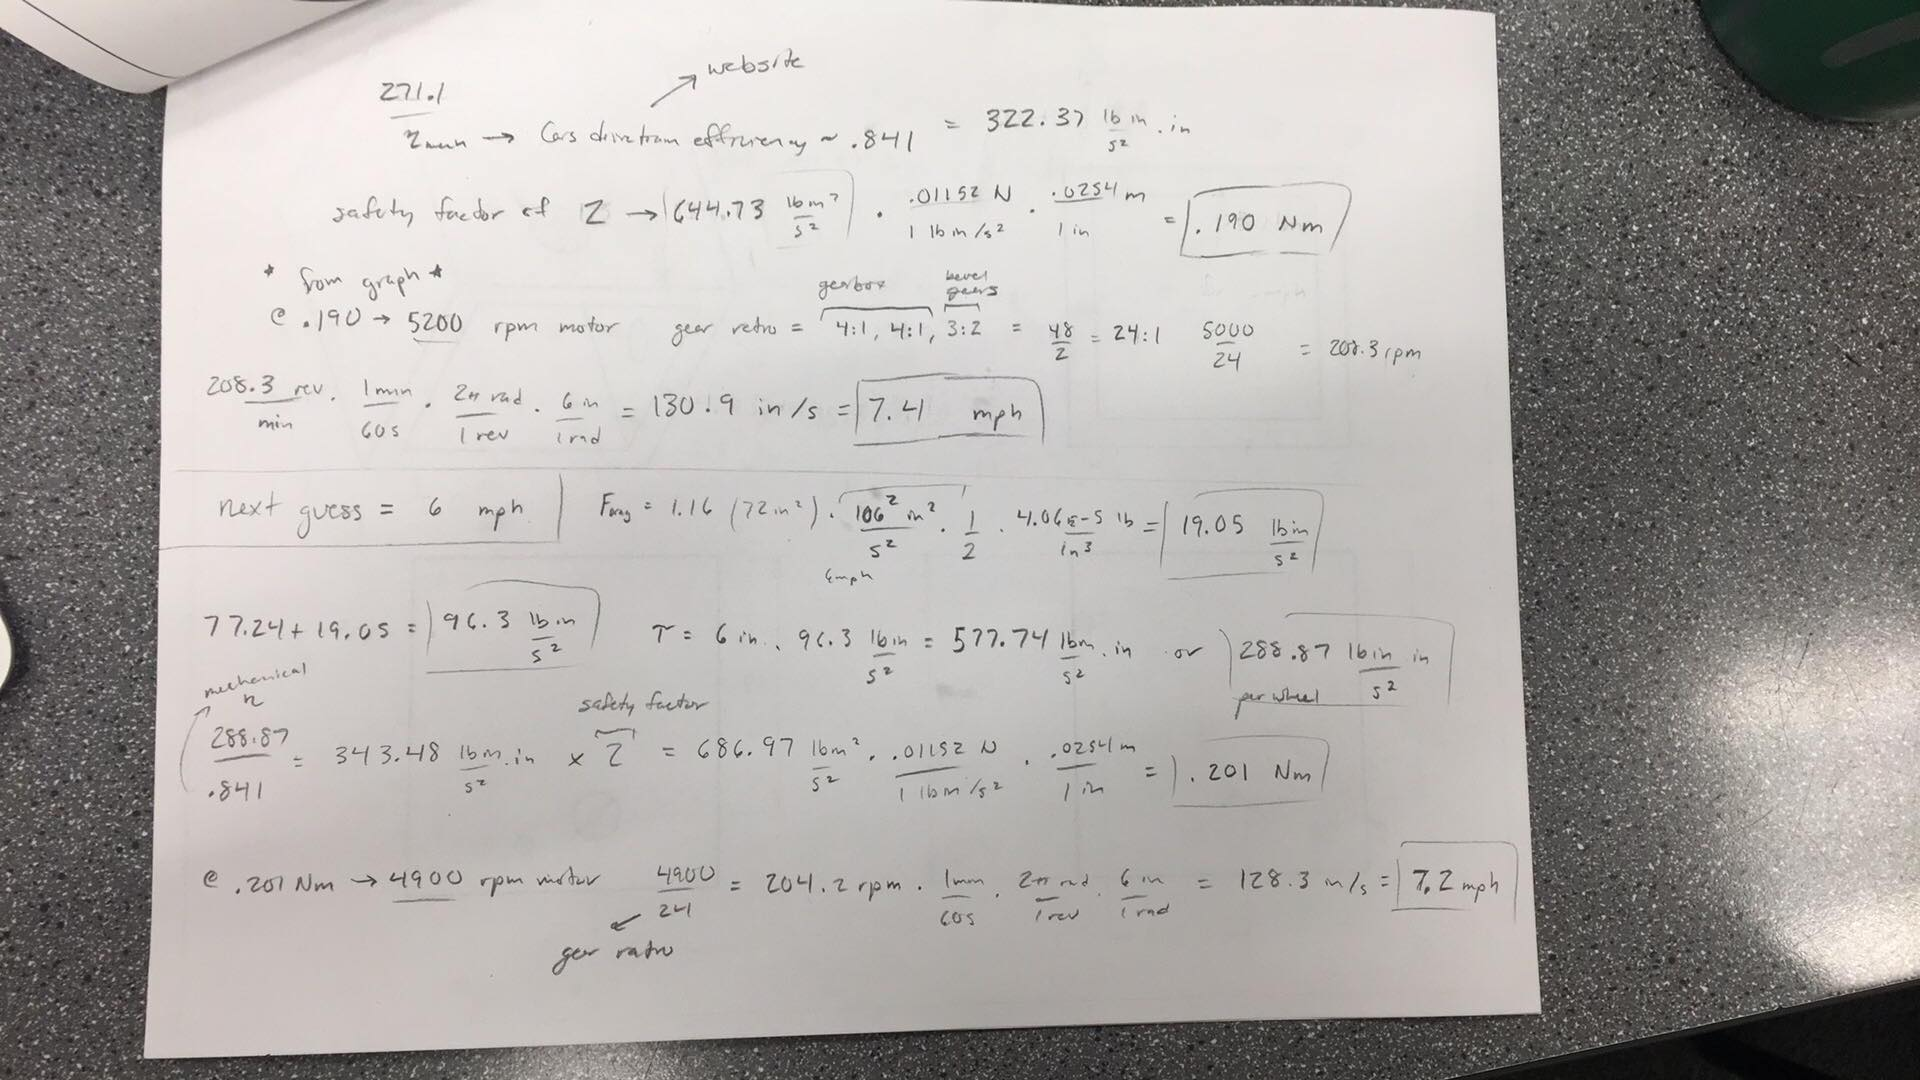
\includegraphics[width=\linewidth]{calculations2}
    \caption{Numerical Values and Solutions, Part II}
\end{figure}

\vfill
\newpage

\begin{figure}[ht]
    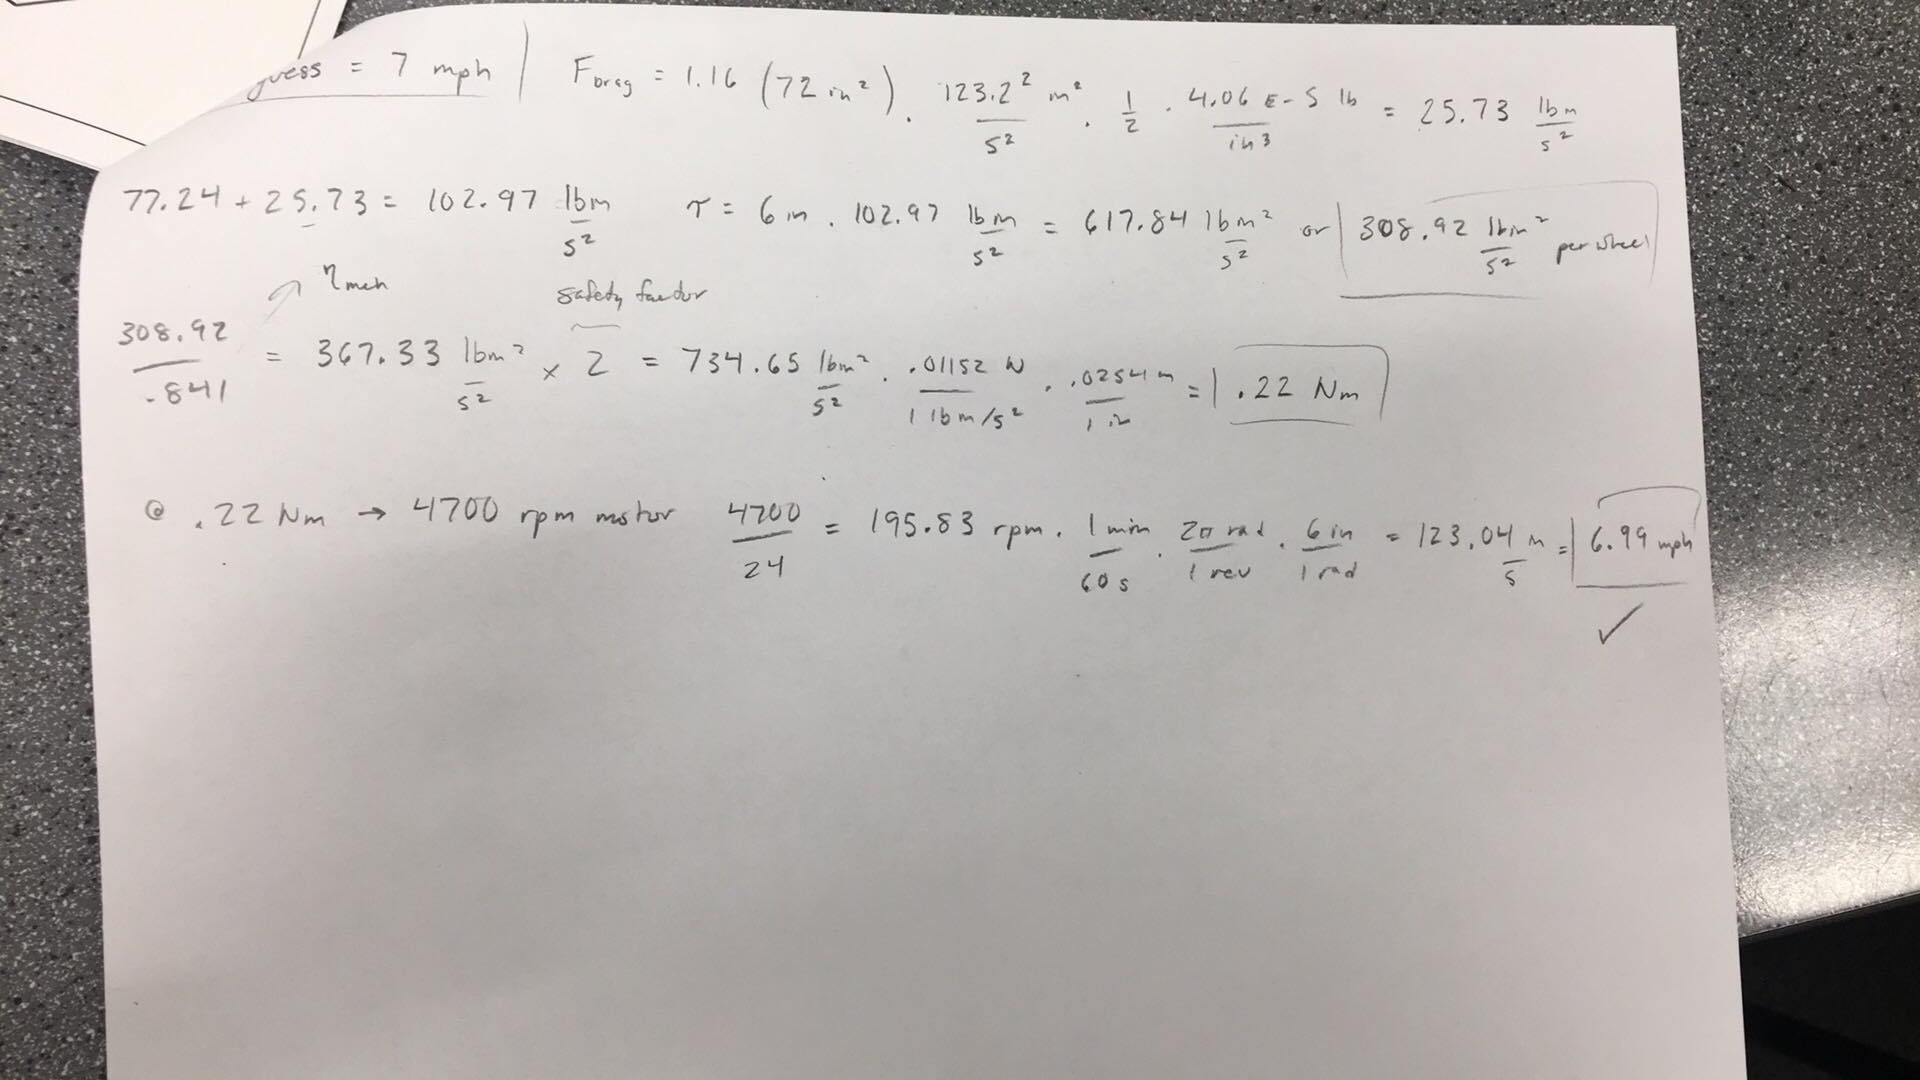
\includegraphics[width=\linewidth]{Calculations3}
    \caption{Numerical Values and Solutions, Part III}
\end{figure}

\vfill
\newpage

\begin{figure}[ht]
    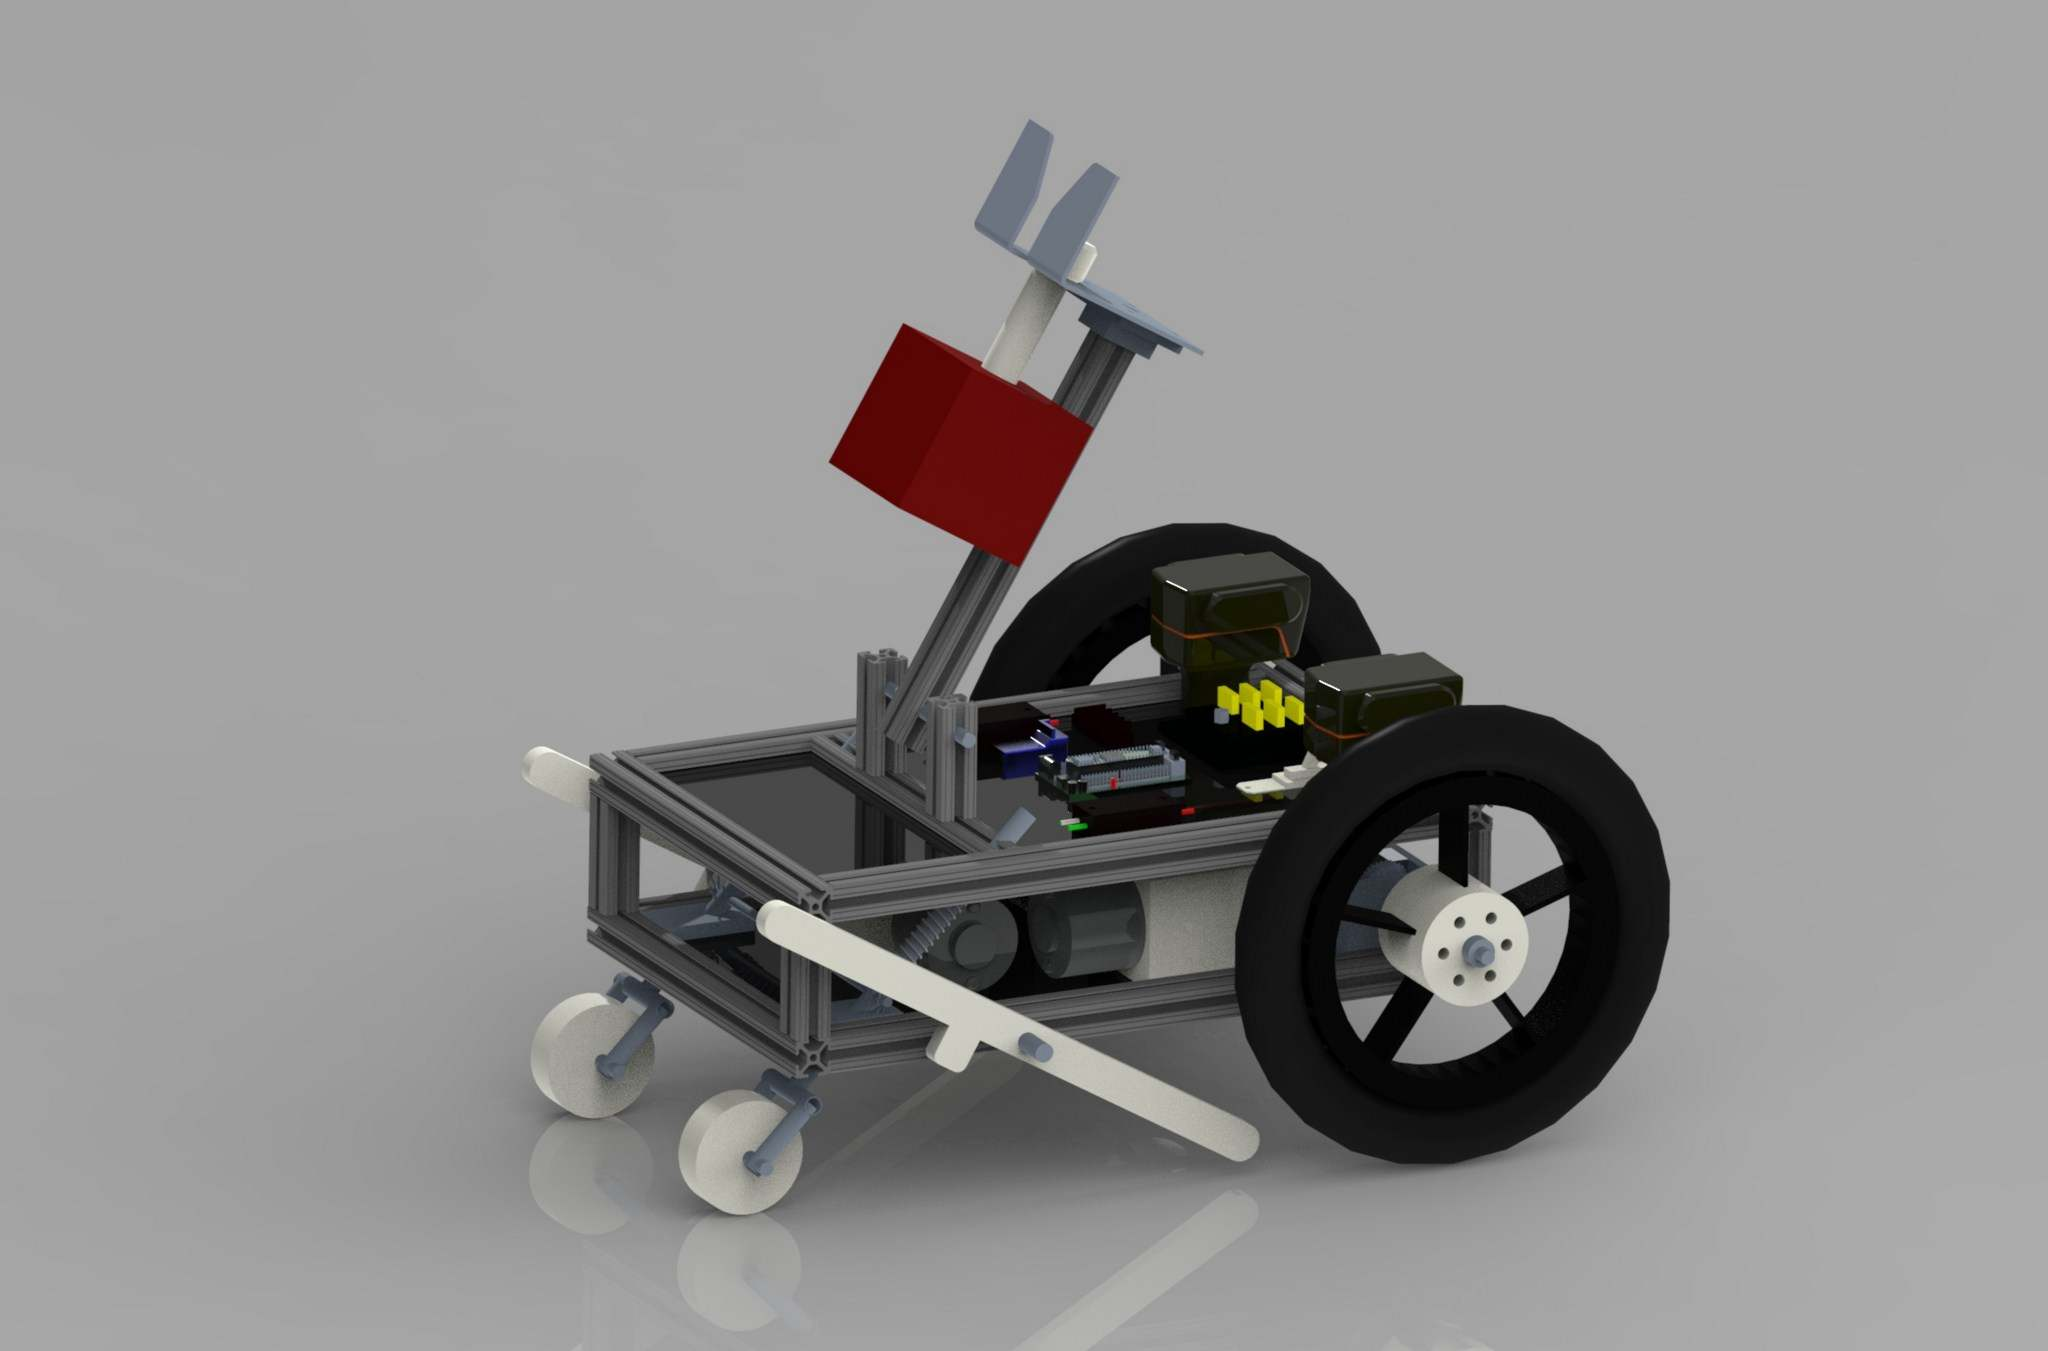
\includegraphics[width=\linewidth]{medkit_arm}
    \caption{Medical Kit Arm}
\end{figure}

\vfill
\newpage

\label{fig:GearStress}
\begin{figure}[ht]
    \includegraphics[width=\linewidth]{GearStress}
    \caption{Gear Stress Calculations}
    \label{fig:GearStress}
\end{figure}

\vfill
\newpage
\clearpage
\end{landscape}
%\subsection{Logbook}
% \begin{longtable}
%     %\csvautotabular{./resources/logbook_v2.csv}
%     \csvautolongtable{./resources/logbook_v2.csv}
% \end{longtable}


\csvreader[
  longtable=lrrrr,
  table head=
    \toprule\bfseries Item &\bfseries Alpha category (\%) \\ \midrule\endhead
    \bottomrule\endfoot,
  late after line=\\,
  before reading={\catcode`\#=12},after reading={\catcode`\#=6}
]{./resources/logbook_v2.csv}{1=\Item,2=\Percentage}{\Item & \Percentage}
\begin{landscape}
\subsection{Bill of Materials}
% Please add the following required packages to your document preamble:
% \usepackage{lscape}
% \usepackage{longtable}
% Note: It may be necessary to compile the document several times to get a multi-page table to line up properly
{\footnotesize
\begin{longtable} {llllll}
\hline
Part Number & Part Name                    & Description                          & Quantity & Price Per Unit & Cost    \\ \hline
\endfirsthead
%
\endhead
%
\hline
\endfoot
%
\endlastfoot
%
6529K11     & Metal Miter Gear             & 16 Pitch, 16 Teeth                   & 2        & \$25.32        & \$50.64 \\
6529K16     & Metal Miter Gear             & 16 Pitch, 24 Teeth                   & 2        & \$32.86        & \$65.72 \\
8619K851    & HDPE Sheet                   & 6"x12"x1"                            & 1        & \$20.01        & \$20.01 \\
9657K435    & 6-Pack, Compression Spring   & 3", 0.66" OD                         & 1        & \$7.82         & \$7.82  \\
9657K437    & 6-Pack, Compression Spring   & 3", 0.72" OD                         & 1        & \$8.86         & \$8.86  \\
9620K25     & Steel Compression Spring     & 3", 0.781" OD                        & 1        & \$4.37         & \$4.37  \\
9414T8      & Set Screw Collar             & 3/8" Diameter                        & 8        & \$1.30         & \$10.40 \\
92391A120   & 25-Pack Hairpin Cotter Pin   & 1/4"-1/2" Clevis Diameter            & 1        & \$8.00         & \$8.00  \\
92949A540   & 50-Pack Button Head Screw    & 1/4"-20, 3/4" Long                   & 1        & \$7.39         & \$7.39  \\
87225K62    & Clear Polycarbonate Sheet    & 12"x24"x1/4"                         & 1        & \$26.13        & \$26.13 \\
8624K46     & HDPE Rod                     & 3"x1'                                & 1        & \$23.10        & \$23.10 \\
6546K31     & 6061 Aluminum Rect. Tube     & 1/4" thick, 2.5"x2.5", 1/2'          & 1        & \$19.08        & \$19.08 \\
47065T68    & T-Slotted Framing            & 1"x1/2"x2'                           & 1        & \$7.98         & \$7.98  \\
6338K414    & Sleeve Bearing               & 3/8" SD, 1/2" HD, 1/4" long          & 4        & \$0.74         & \$2.96  \\
7297K15     & Plastic Miter Gear           & 24 Pitch, 24 Teeth                   & 2        & \$5.39         & \$10.78 \\
7297K17     & Plastic Miter Gear           & 24 Pitch, 36 Teeth                   & 2        & \$5.44         & \$10.88 \\
6338K411    & Sleeve Bearing               & 1/4" SD, 3/8" HD                     & 4        & \$0.67         & \$2.68  \\
6338K462    & Sleeve Bearing               & 7/16" SD, 9/16" HD                   & 4        & \$1.12         & \$4.48  \\
47065t95    & 1" 80/20                     & 2ft long                             & 1        & \$7.79         & \$7.79  \\
6338K421    & Sleeve Bearing               & 1/2'' SD, 5/8'' HD, 1'' long         & 2        & \$1.44         & \$2.88  \\
1346K18     & Steel Shaft                  & 1/2" diameter, 24" long              & 1        & \$17.47        & \$17.47 \\
8671K73     & HDPE Bar                     & 4"x1/2"x4'                           & 4        & \$5.29         & \$21.16 \\
92949A540   & 50-Pack Button Head Screw    & 1/4"-20, 3/4" Long                   & 1        & \$7.39         & \$7.39  \\
98381A508   & 50-Pack Dowel Pin            & 3/16" diameter, 3/4" long            & 1        & \$7.80         & \$7.80  \\
8893K178    & Drill Rod                    & 0.1875" diameter, 3' long            & 1        & \$4.30         & \$4.30  \\
47065T95    & T-Slotted Framing            & 1" High x 1" Wide, Solid             & 1        & \$7.79         & \$7.79  \\
89015K18    & 6061 Aluminum Sheet          & 1/8" Thick, 12" x 12"                & 1        & \$27.71        & \$27.71 \\
6338K312    & Brass Flanged Sleeve Bearing & 5/8" Flange OD                       & 6        & \$1.12         & \$6.72  \\
9414T8      & Set Screw Shaft Collar       & for 3/8" Diameter, 1215 Carbon Steel & 2        & \$1.30         & \$2.60  \\ \hline
\end{longtable}
\end{landscape}
}
\subsection{Appendix II: Code (DynaSaRR.ino)}
\begin{lstlisting}[style=myArduino]
#include <Servo.h>

bool atWall = false;
bool firstStep = false;
bool secondStep = false;
bool overTheWall = false;
bool inTheChute = false;
bool throughTheChute = false;
bool medkitPlaced = false;

int Ch1, Ch2, Ch3, Ch4, Ch5, Ch6; // hold receiver signals
int R_wheel;
int L_wheel;
int Medkit_arm;
int Lifting_arm;
 
Servo L_Servo;
Servo R_Servo;
Servo Lifting_Servo;
Servo Medkit_Servo;

const int R_lightSensorPin = A9;
const int L_lightSensorPin = A8;
const int F_distSensorPin = A7;
const int R_distSensorPin = A6;
const int L_distSensorPin = A5;

const int R_ServoPin = A12;
const int L_ServoPin = 1;
const int Lifting_ServoPin = 2;
const int Medkit_ServoPin = 3;
const int front_limitSwitchPin = 4;
const int back_limitSwitchPin = 5;

const int Ch1Pin = 7;   // channel 1 is right stick lateral
const int Ch2Pin = 8;   // channel 2 is right stick vertical
const int Ch3Pin = 9;   // channel 3 is left stick vertical
const int Ch4Pin = 10;  // channel 4 is left stick lateral
const int Ch5Pin = 11;  // channel 5 is right knob
const int Ch6Pin = 12;  // channel 6 is left knob
const int onBoardLEDPin = 13;

// Servo control must fall between 1000uS (full reverse) and 2000uS (full forward)
const int ServoLow = 1000;
const int ServoHigh = 2000;
const int ServoZero = 1500;
const int ServoHalfRange = 500;

const int transmitterTimeout = 21000;

const int autonomousActivationFrequency = 1800; // knob turned completely clockwise

const int distSensorStopValue = 450; // Value of prox sensor indicating stopping distance; 4ish inches
const int distSensorSlowValue = 2000; // 2000 = 1 foot ish
const int lightThreshold = 600;//550; // sensor value for detecting target light (vs. noise/reflection)
const int chuteDistThreshold = 150; // Minimum value of left and right prox sensors for robot to be in chute
const int distSensorMaxValue = 1000;

int L_lightSensor;    // hold photoresistor value
int R_lightSensor;    // hold photoresistor value
int F_distSensor;     // hold front sharp sensor value
int R_distSensor;     // hold right distance sensor value
int L_distSensor;     // hold left distance sensor value
double distDiff;      // difference between dist sensors. if positive, closer to right of chute
int lightSensorDiff;  // difference between L_lightSensor and R_lightSensor
int Lifting_speed;    // speed changes for lifting arm
int Medkit_speed;     // speed changes for Medkit arm

// note: limit switches read 1 when not pressed and 0 when pressed
bool front_limitSwitch;
bool back_limitSwitch;

// setup() runs once then loop() runs
void setup() {
  pinMode(Ch1Pin, INPUT); // channel 1 is right stick lateral
  pinMode(Ch2Pin, INPUT); // channel 2 is right stick vertical
  pinMode(Ch3Pin, INPUT); // channel 3 is left stick vertical
  pinMode(Ch4Pin, INPUT); // channel 4 is left stick lateral
  pinMode(Ch5Pin, INPUT); // channel 5 is right knob
  pinMode(Ch6Pin, INPUT); // channel 6 is left knob

  pinMode(R_lightSensorPin, INPUT); // channel 5 is right knob
  pinMode(L_lightSensorPin, INPUT); // channel 6 is left knob
  pinMode(F_distSensorPin, INPUT);
  pinMode(R_distSensorPin, INPUT);
  pinMode(L_distSensorPin, INPUT);

  pinMode(front_limitSwitchPin, INPUT);
  pinMode(back_limitSwitchPin, INPUT);

  R_Servo.attach(R_ServoPin);
  L_Servo.attach(L_ServoPin);
  Lifting_Servo.attach(Lifting_ServoPin);
  Medkit_Servo.attach(Medkit_ServoPin);

  Lifting_speed = ServoZero;
  Medkit_speed = ServoZero;

  front_limitSwitch = false;
  back_limitSwitch = false;

  //Flash the onboard LED on and Off 10x 
  for (int i = 0; i < 10; i++) {
    digitalWrite(onBoardLEDPin, HIGH);
    delay(100);
    digitalWrite(onBoardLEDPin, LOW);
    delay(100);
  }

  Serial.begin(9600);
}


void driveServosRC() {
  //Serial.println("RC");
  
  if (Ch2 <= ServoZero) {
    L_wheel = Ch1 + Ch2 - ServoZero;
    R_wheel = Ch1 - Ch2 + ServoZero;
  }
  else {
    int Ch1_mod = map(Ch1, ServoLow, ServoHigh, ServoLow, ServoHigh); // Invert CH1 axis to keep the math similar
    int Ch2_mod = map(Ch2, ServoLow, ServoHigh, ServoHigh, ServoLow); // Slow reaction time

    L_wheel = Ch1_mod + Ch2 - ServoZero;
    R_wheel = Ch2_mod - Ch2 + ServoZero;
  }

  int Medkit_arm = Ch3; 
  int Lifting_arm = Ch4;

  front_limitSwitch = digitalRead(front_limitSwitchPin);
  back_limitSwitch = digitalRead(back_limitSwitchPin);

  if (!front_limitSwitch && (Medkit_arm < ServoZero)) {
   Medkit_arm = ServoZero;
  } 
  else if (!back_limitSwitch && (Medkit_arm > ServoZero)) {
   Medkit_arm = ServoZero;
  }

  constrain(L_wheel, ServoLow, ServoHigh);
  constrain(R_wheel, ServoLow, ServoHigh);
  constrain(Lifting_arm, ServoLow, ServoHigh);
  constrain(Medkit_arm, ServoLow, ServoHigh);

  L_Servo.writeMicroseconds(L_wheel);
  R_Servo.writeMicroseconds(R_wheel);
  Lifting_Servo.writeMicroseconds(Lifting_arm);
  Medkit_Servo.writeMicroseconds(Medkit_arm);
}

void printRC() {
  Serial.println(" RC Control Mode ");
  Serial.print("Value Ch1 = ");
  Serial.println(Ch1);
  Serial.print("Value Ch2 = ");
  Serial.println(Ch2);
  Serial.print("Value Ch3 = ");
  Serial.println(Ch3);
  Serial.print("Value Ch4 = ");
  Serial.println(Ch4);
  Serial.print("Value Ch5 = ");
  Serial.println(Ch5);
  Serial.print("Value Ch6 = ");
  Serial.println(Ch6);
  delay(1000);
}

void printSensors() {
  Serial.print("Left Sensor = ");
  Serial.println(L_lightSensor);
  Serial.print("Right Sensor = ");
  Serial.println(R_lightSensor);


  Serial.print("Front Distance = ");
  Serial.println(F_distSensor);
  Serial.print("Left Distance = ");
  Serial.println(L_distSensor);
  Serial.print("Right Distance = ");
  Serial.println(R_distSensor);

  Serial.print("Front Limit Switch: ");
  Serial.println(front_limitSwitch);
  Serial.print("Back Limit Switch: ");
  Serial.println(back_limitSwitch);
}

void updateSensors() {
  L_lightSensor = analogRead(L_lightSensorPin);
  R_lightSensor = analogRead(R_lightSensorPin);

  lightSensorDiff = abs(L_lightSensor - R_lightSensor);

  F_distSensor = analogRead(F_distSensorPin);

  for (int i = 0; i < 4; i++) {
    F_distSensor += analogRead(F_distSensorPin);
    R_distSensor += analogRead(R_distSensorPin);
    L_distSensor += analogRead(L_distSensorPin);
  }
  F_distSensor /= 5;
  R_distSensor /= 5;
  L_distSensor /= 5;

  distDiff = R_distSensor - L_distSensor;

  front_limitSwitch = digitalRead(front_limitSwitchPin);
  back_limitSwitch = digitalRead(back_limitSwitchPin);
  
  delay(100);
}

void turnLeft(int runTime, double percent) {
  int r = ServoZero - ServoHalfRange*percent;
  int l = ServoZero - ServoHalfRange*percent - 25; // constant offset to account for difference in speeds (from direction of rotation)

  constrain(r, ServoLow, ServoHigh);
  constrain(l, ServoLow, ServoHigh);

  R_Servo.writeMicroseconds(r);
  L_Servo.writeMicroseconds(l);

  delay(runTime);
}

void turnRight(int runTime, double percent) {
  int r = ServoZero + ServoHalfRange*percent + 25;
  int l = ServoZero + ServoHalfRange*percent;

  constrain(r, ServoLow, ServoHigh);
  constrain(l, ServoLow, ServoHigh);

  R_Servo.writeMicroseconds(r);
  L_Servo.writeMicroseconds(l);

  delay(runTime);
}

void driveForward(int runTime, double percent) {
  int r = ServoZero - ServoHalfRange*percent;
  int l = ServoZero + ServoHalfRange*percent;

  constrain(r, ServoLow, ServoHigh);
  constrain(l, ServoLow, ServoHigh);

  R_Servo.writeMicroseconds(r);
  L_Servo.writeMicroseconds(l);

  delay(runTime);
}

void driveBackward(int runTime, double percent) {
  int r = ServoZero + ServoHalfRange*percent;
  int l = ServoZero - ServoHalfRange*percent;

  constrain(r, ServoLow, ServoHigh);
  constrain(l, ServoLow, ServoHigh);

  R_Servo.writeMicroseconds(r);
  L_Servo.writeMicroseconds(l);

  delay(runTime);
}

void stopDriving(int runTime) {
  L_Servo.writeMicroseconds(ServoZero);
  R_Servo.writeMicroseconds(ServoZero);

  delay(runTime);
  // Serial.println("StopDriving");
}

void medkitArmForward(int runTime, double percent) {
  if (front_limitSwitch) {
    int medkitSpeed = ServoZero - ServoHalfRange * percent;

    Medkit_Servo.writeMicroseconds(medkitSpeed);

    //Serial.println("Medkit Forward");
    delay(runTime);
  }
  else {
    medkitArmStop(runTime);
  }
}

void medkitArmBackward(int runTime, double percent) {
  if (back_limitSwitch) {
    int medkitSpeed = ServoZero + ServoHalfRange * percent;

    Medkit_Servo.writeMicroseconds(medkitSpeed);

    //Serial.println("Medkit Backward");
    delay(runTime);
  }
  else {
    medkitArmStop(runTime);
  }
}

void medkitArmStop(int runTime) {
  Medkit_Servo.writeMicroseconds(ServoZero);

  //Serial.println("Medkit Stop");
  delay(runTime);
}

void liftingArmForward(int runTime, double percent) {
  Lifting_arm = ServoZero - ServoHalfRange*percent;
  constrain(Lifting_arm, ServoLow, ServoHigh);
  Lifting_Servo.writeMicroseconds(Lifting_arm);
  delay(runTime);
}

void liftingArmStop(int runTime) {
  Lifting_arm = ServoZero;
  Lifting_Servo.writeMicroseconds(Lifting_arm);
  delay(runTime);
}

void steps(int runTime) {
  Lifting_arm = ServoZero - ServoHalfRange*(.75);
  int r = ServoZero - ServoHalfRange*(.25);
  int l = ServoZero + ServoHalfRange*(.25);
  constrain(Lifting_arm, ServoLow, ServoHigh);
  constrain(r, ServoLow, ServoHigh);
  constrain(l, ServoLow, ServoHigh);

  R_Servo.writeMicroseconds(r);
  L_Servo.writeMicroseconds(l);
  Lifting_Servo.writeMicroseconds(Lifting_arm);
  delay(runTime);
}

void overWall(int runTime) {
  int r = ServoZero - ServoHalfRange - 50;
  int l = ServoZero + ServoHalfRange + 100;
  Lifting_arm = ServoZero - ServoHalfRange - 50;

  Lifting_Servo.writeMicroseconds(Lifting_arm);
  R_Servo.writeMicroseconds(r);
  L_Servo.writeMicroseconds(l);
  
  delay(runTime);
  liftingArmStop(50);
  stopDriving(50);
}

void autonomousLightSeekingNew() {
  const int chuteEntranceThreshold = 100;
  const int distDiffThreshold = 70;
  const int chuteThreshold = 70;

  const int lightSensorMaxValue = 900;
  const int lightSensorDiffThreshold = 40;

  if ((L_lightSensor > R_lightSensor) && (-lightSensorDiff > lightSensorDiffThreshold)) {
    double r_speed = map(-lightSensorDiff, 0, distSensorMaxValue, 0.1, 1);
    turnRight(10, r_speed);
  }
  else if ((R_lightSensor > L_lightSensor) && (lightSensorDiff > lightSensorDiffThreshold)) {
    double l_speed = map(lightSensorDiff, 0, lightSensorMaxValue, 0.1, 1);
    turnLeft(10, l_speed);
  }
  else {
    driveForward(10, 0.2);
  }
}

void autonomousLightSeeking() {
  if(medkitPlaced == false) {
    if (F_distSensor < distSensorStopValue) {
      //Serial.println("1");
      if (R_lightSensor <= lightThreshold) {
        stopDriving(10);
        //Serial.println(F_distSensor);
        if (lightSensorDiff > 50 ) {
          if (L_lightSensor > R_lightSensor) {
            delay(50);
            turnLeft(150, 0.2); // 0.1 is too low--doesn't drive
            driveForward(100, 0.2);
            //Serial.println("turn left");
          }
          else {
            delay(50);
            turnRight(200, 0.2);
            driveForward(100, 0.2);
            //Serial.println("turn right");
          }
        }
        else {
          driveForward(200, 0.2); // works on 2000 but takes too long to recognize distance
          //Serial.println("forward");
        }
      } 
      else {
        turnRight(10, 0.2);
        //Serial.println("lost");
        updateSensors();
      }
    }
    else {
      stopDriving(100);
      delay(500);
      placeMedkit();
    }
  }
}

void chuteTraverse() {
  if(inTheChute == false) {
    driveForward(100, 0.2);
    if(R_distSensor > 150) {
      if(L_distSensor > 150) {
        inTheChute = true;
        //Serial.println("in");
      }
    }
  }
   else if(R_distSensor > 100) {
    if(L_distSensor > 100) {
      if(distDiff > 75) { // around 2in difference
        turnLeft(5, 0.21);
        //Serial.println("turning left");
      }
      else if(distDiff < -75) {
        turnRight(5, 0.2);
        //Serial.println("turning right");
      }
      else {
        //Serial.println("driving forward");
        driveForward(10, 0.18);
      }
    }
   }
  else {
    //Serial.println("out of chute");
    driveForward(500, 0.22);
    stopDriving(100);
    turnRight(250, .22);
    //stopDriving(500);
    throughTheChute = true;
  }
}

void wallTraverse() {
  if(F_distSensor < 450 && !atWall) {
    driveForward(100, 0.2);
  }
  else {
    atWall = true;
  }
  
  if(atWall && !firstStep) {
    steps(800); // first step
    firstStep = true;
    stopDriving(10);
    liftingArmStop(10);
    delay(500);
  }
  else if(atWall && !secondStep) {
    steps(750);
    secondStep = true;
    stopDriving(10);
    liftingArmStop(10);
    delay(500);
  }
  else if(atWall && !overTheWall) {
    //driveForward(200, 0.3); //THIS MIGHT NEED TO BE COMMENTED BACK IN
    overWall(2750);
    stopDriving(10);
    liftingArmStop(10);
    delay(500);        
    overTheWall = true;
    stopDriving(10);
    liftingArmStop(10);
    delay(250);
  }
  else if(overTheWall) {
    stopDriving(10);
    liftingArmStop(10);
  }
  
}

void placeMedkit() {
  medkitArmForward(500, 0.05); // tighten chain
  delay(100);
  medkitArmForward(250, 0.45);
  delay(100);
  medkitArmForward(250, 0.10);
  delay(250);
  
  medkitArmStop(500);
  driveBackward(100, 0.1);

  delay(500);
  
  medkitArmStop(100);
  stopDriving(100);
  medkitPlaced = true;
}

void autonomousMode() {
  updateSensors();
  //Serial.println(distDiff);

  if (!overTheWall) {
    wallTraverse();
  }
  else if (overTheWall) {
    chuteTraverse();
  }
  if (throughTheChute && !medkitPlaced) {
    Serial.println("light");
    autonomousLightSeeking();
  }
  //Serial.println("Autonomous");
}

void loop() {
  Ch5 = pulseIn(Ch5Pin, HIGH, transmitterTimeout); // ch 5 toggles autonomous mode
  Ch6 = pulseIn(Ch6Pin, HIGH, transmitterTimeout); // ch 6 fully clockwise resets medkitPlaced

  updateSensors();

  // do nothing if the controller is disconnected
  if (Ch5 < ServoLow) {
    stopDriving(10);
    medkitArmStop(10);
    liftingArmStop(10);
  } 
  else {
    if (Ch6 <= autonomousActivationFrequency) {
      medkitPlaced = false;
      inTheChute = false;
      throughTheChute = false;
      atWall = false;
      firstStep = false;
      secondStep = false;
      overTheWall = true;
    }
    
    if (Ch5 <= autonomousActivationFrequency) {
      autonomousMode();
    }
    else {
      Ch1 = pulseIn(Ch1Pin, HIGH, transmitterTimeout);
      Ch2 = pulseIn(Ch2Pin, HIGH, transmitterTimeout);
      Ch3 = pulseIn(Ch3Pin, HIGH, transmitterTimeout);
      Ch4 = pulseIn(Ch4Pin, HIGH, transmitterTimeout);

      driveServosRC();
    }
  }
}
\end{lstlisting}

\newpage
\subsection{Appendix III: Part and Sub-Assembly Drawings}

\begin{landscape}
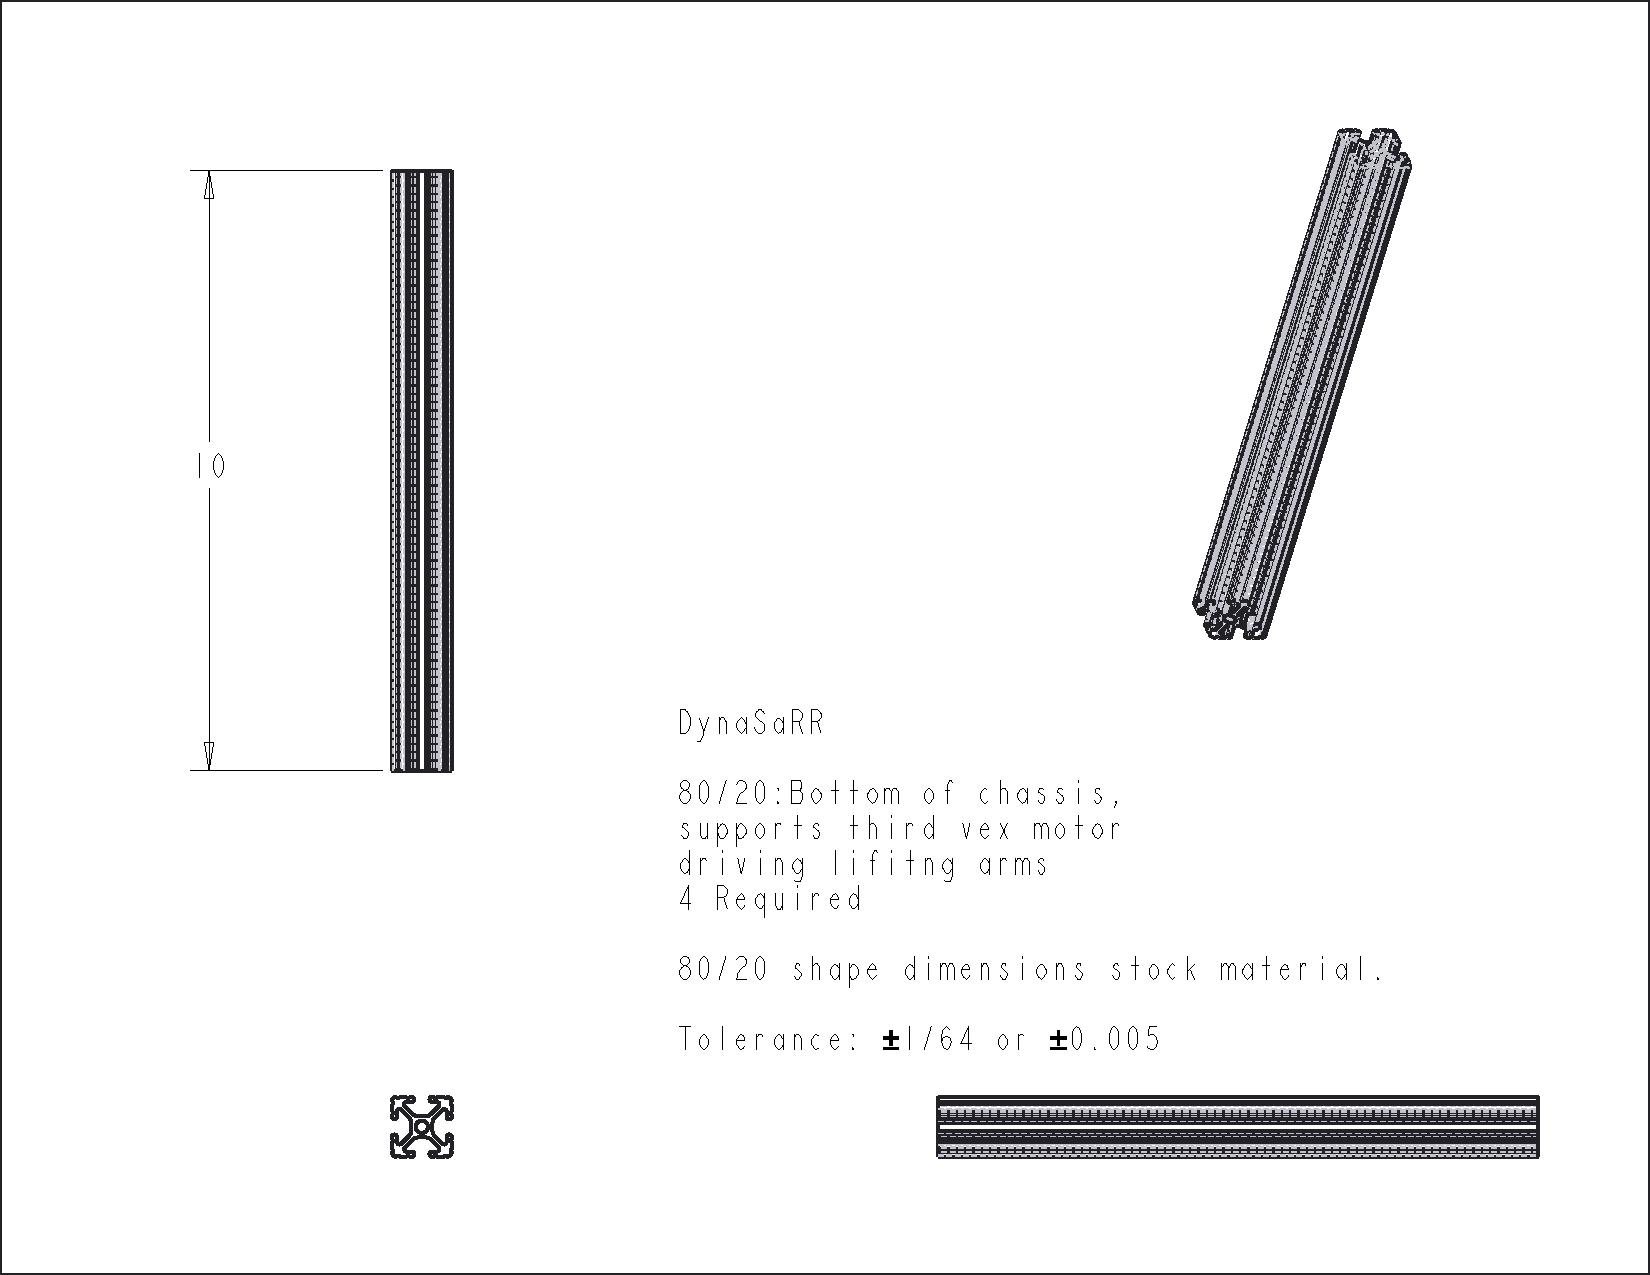
\includepdf[pages={-},angle=90]{./drawings/1010_10_drawing}
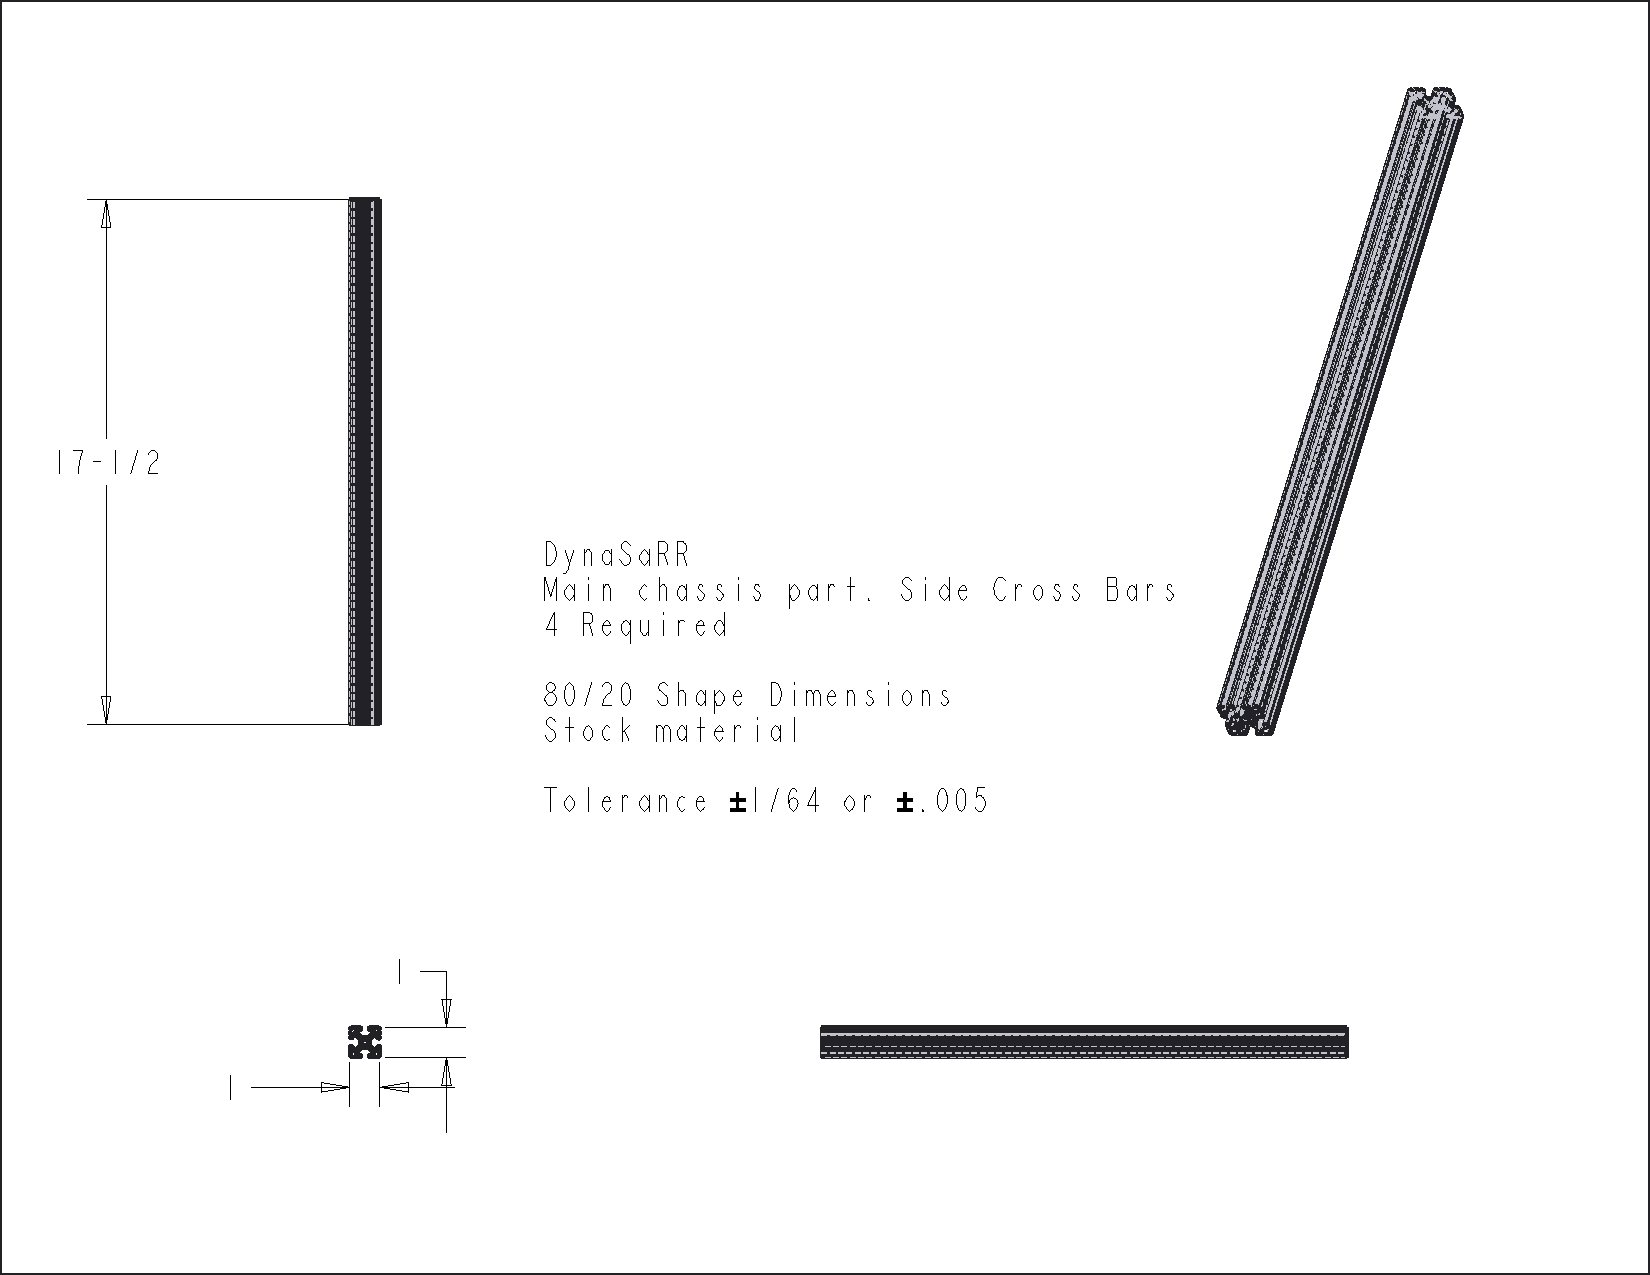
\includepdf[pages={-},angle=90]{./drawings/1010_14_drawing}
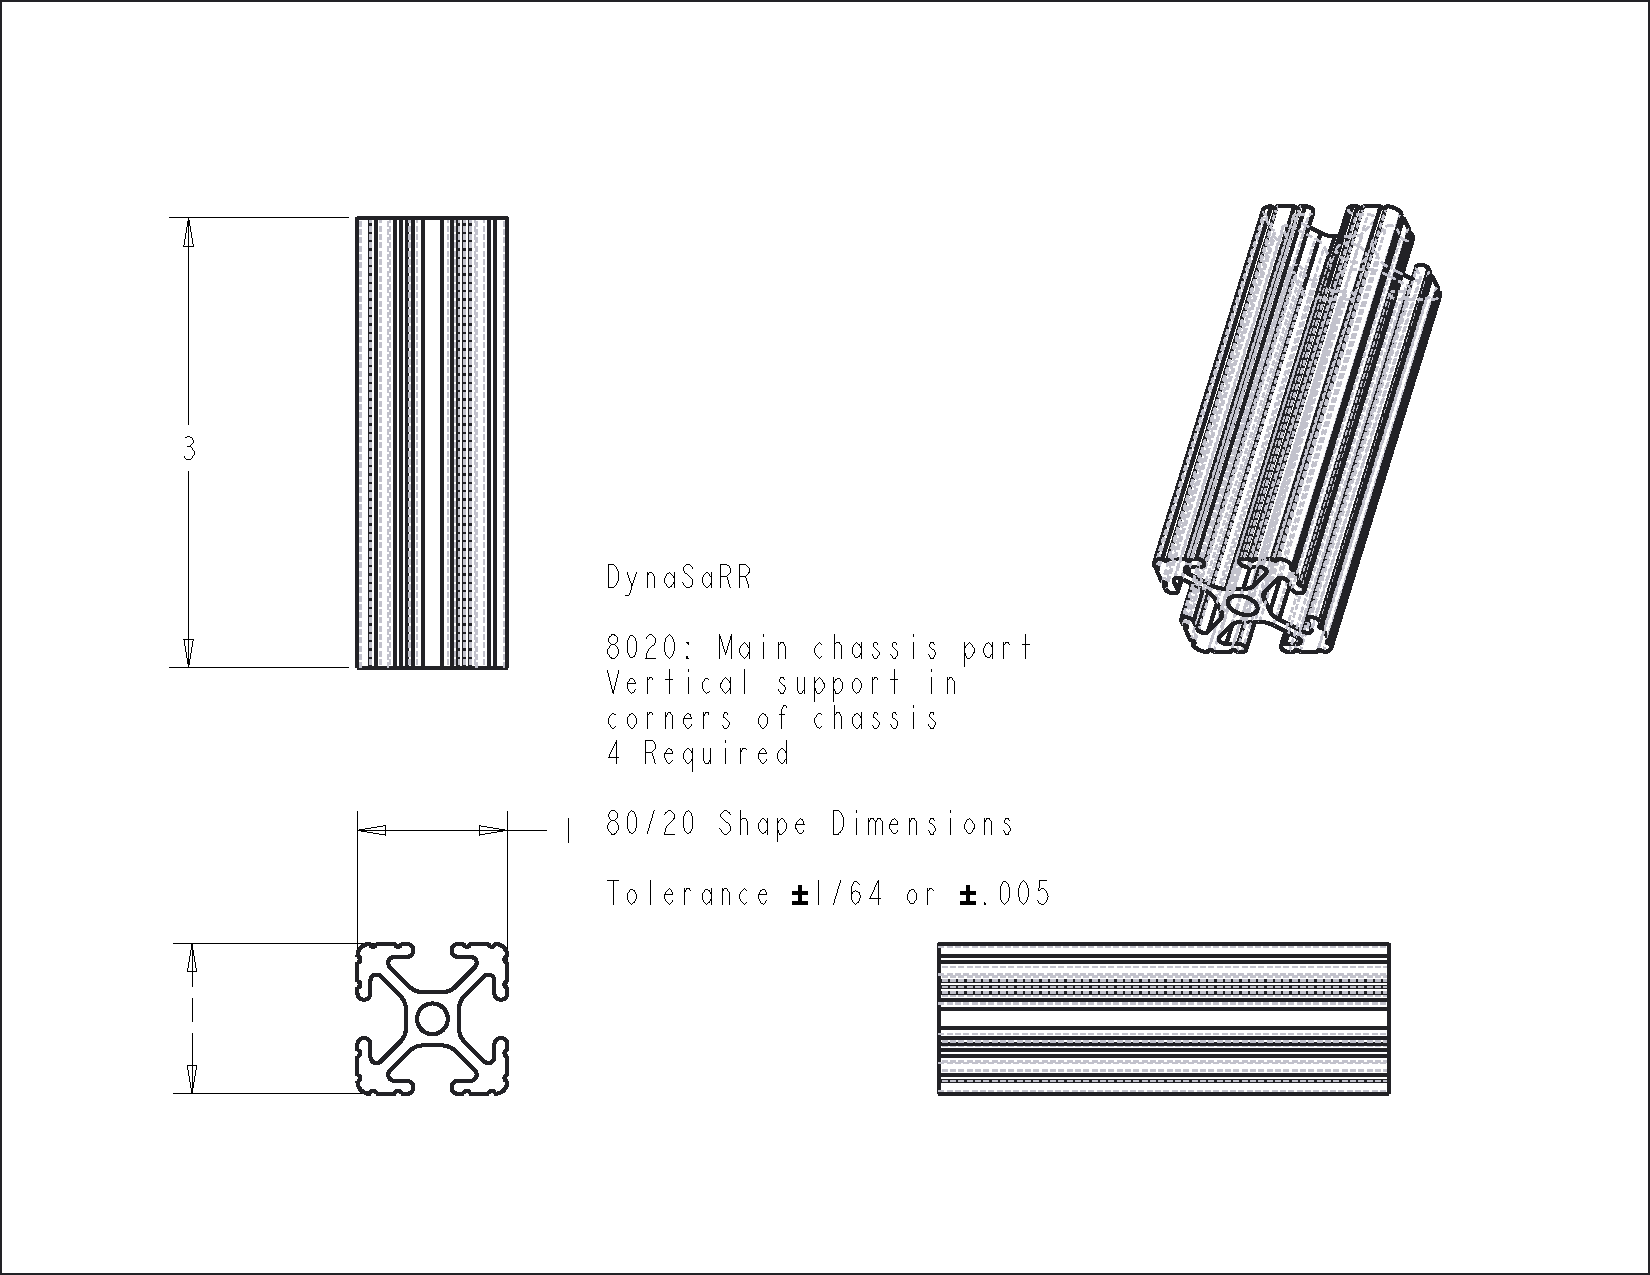
\includepdf[pages={-},angle=90]{./drawings/1010_3_drawing}
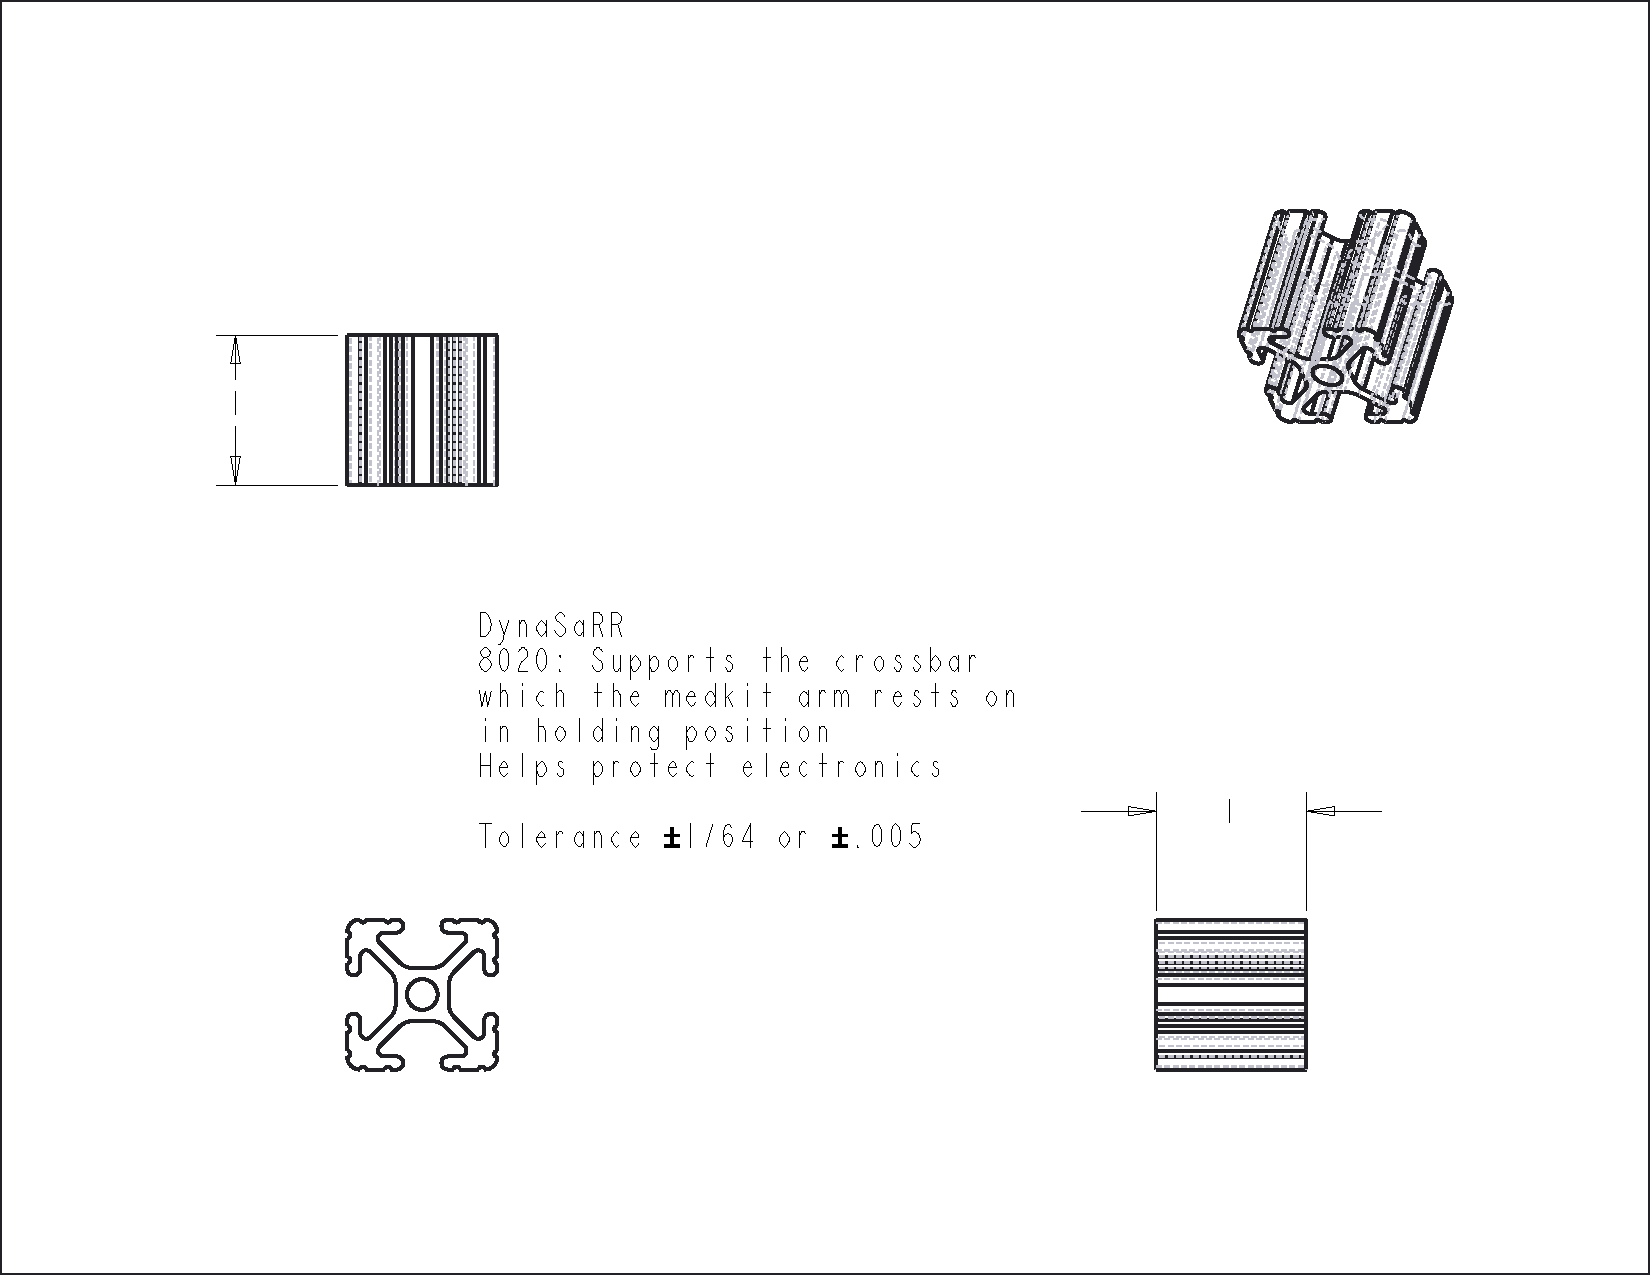
\includepdf[pages={-},angle=90]{./drawings/1010_medkit_rester_drawing}
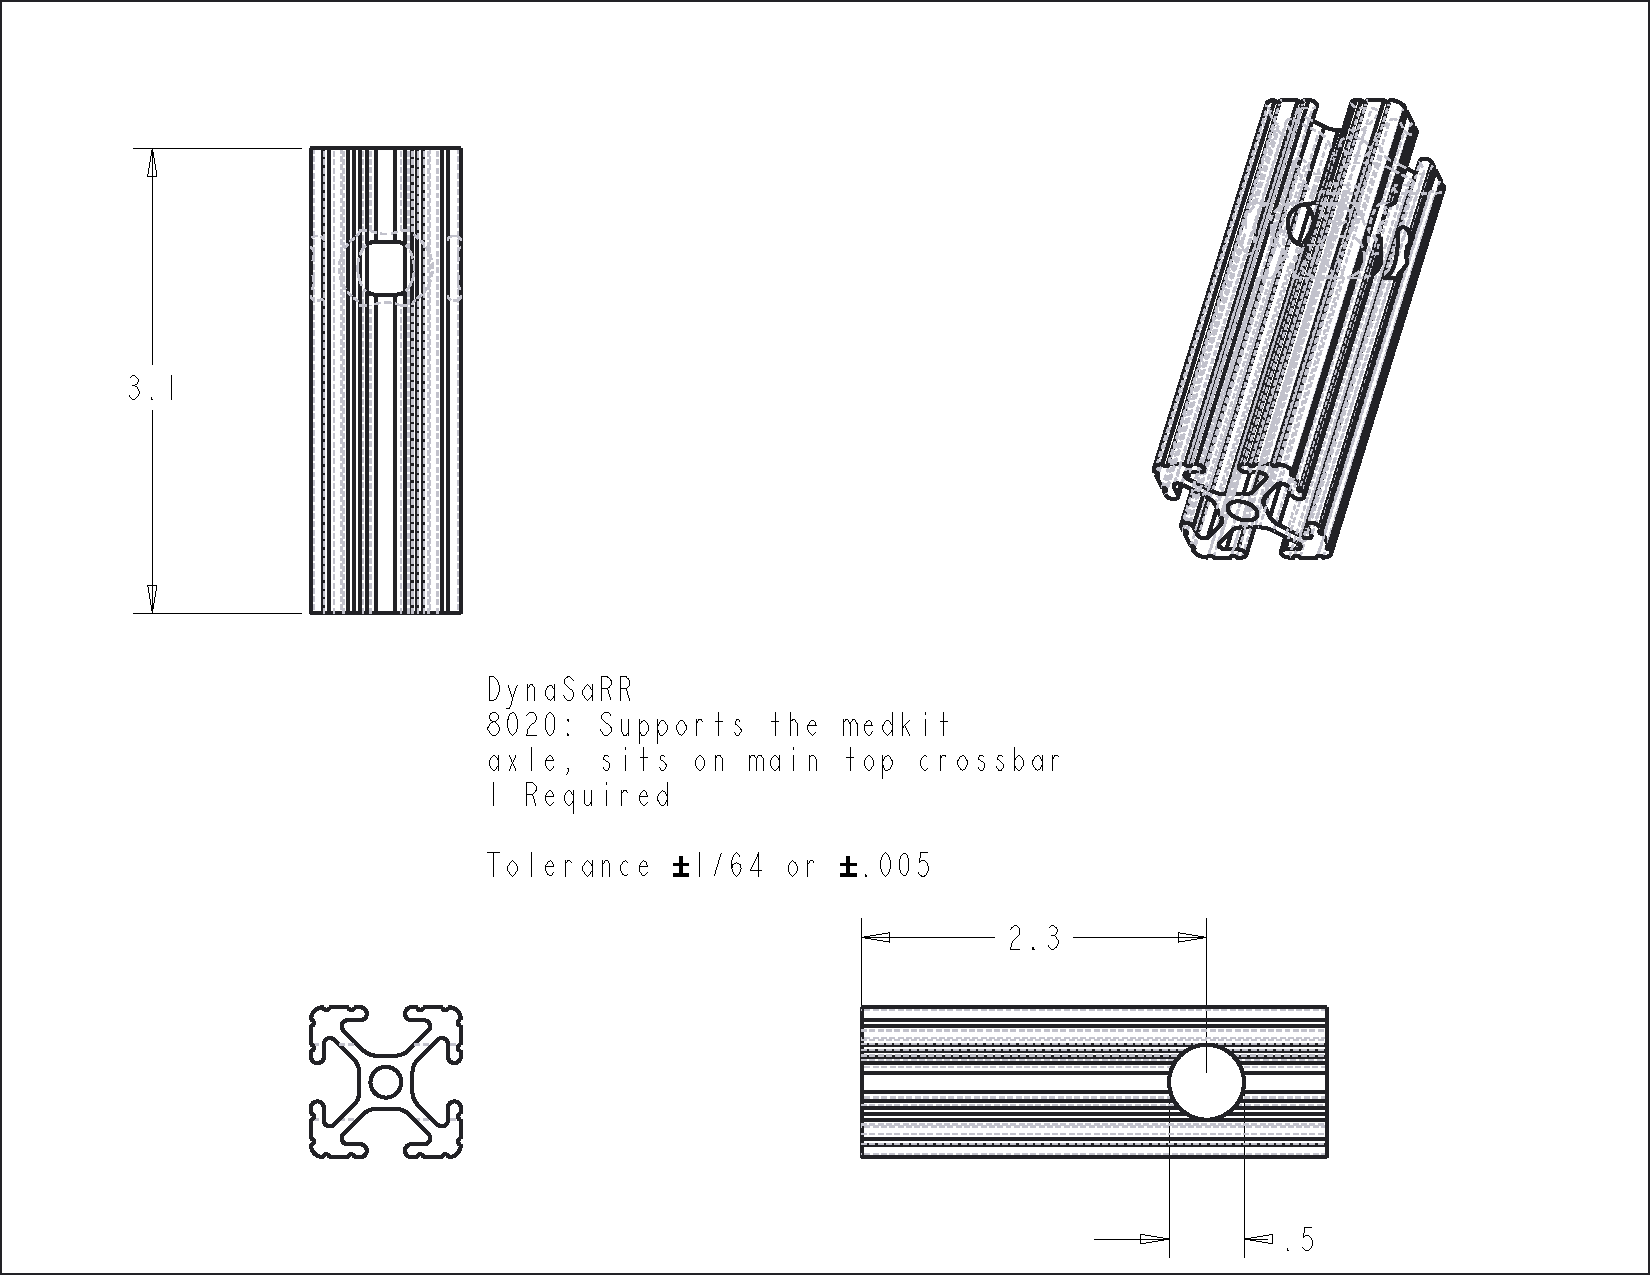
\includepdf[pages={-},angle=90]{./drawings/1010_medkit_support_drawing}
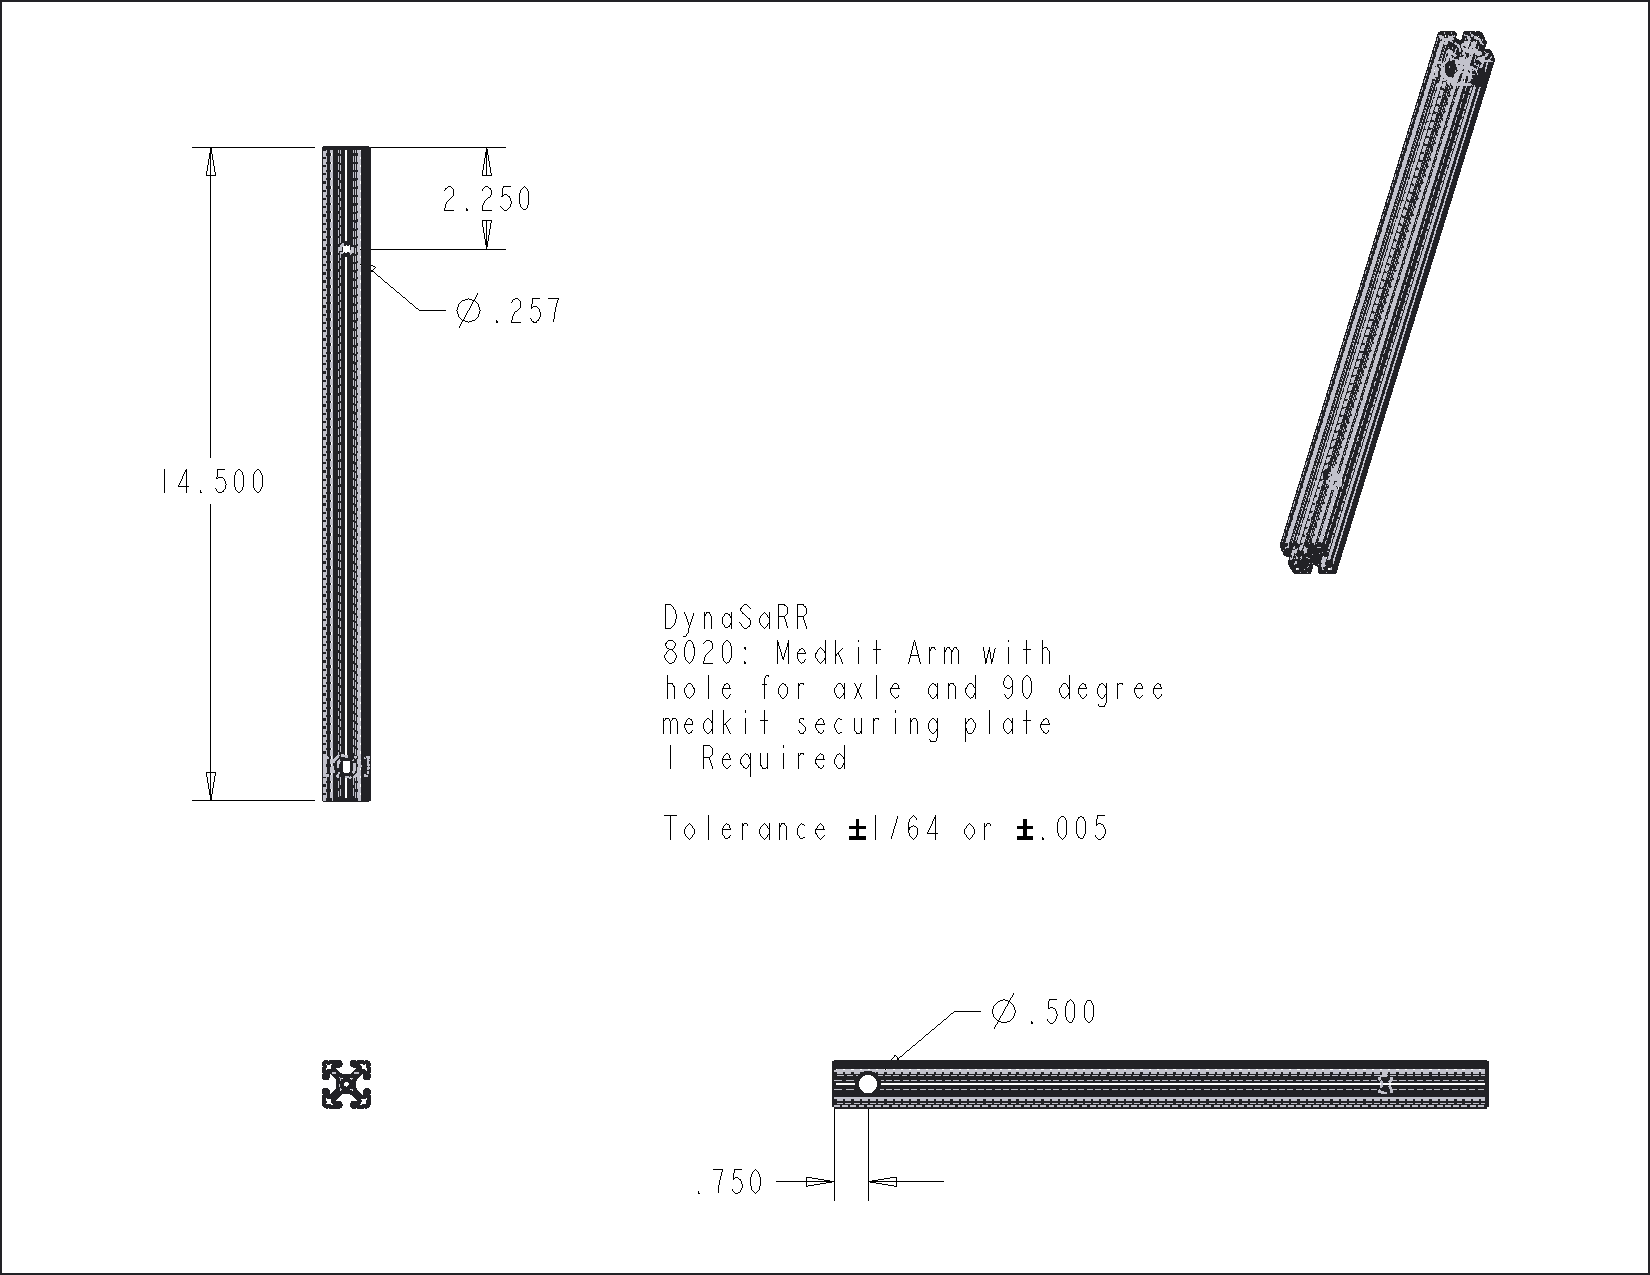
\includepdf[pages={-},angle=90]{./drawings/1010_medkitarm_final_drawing}
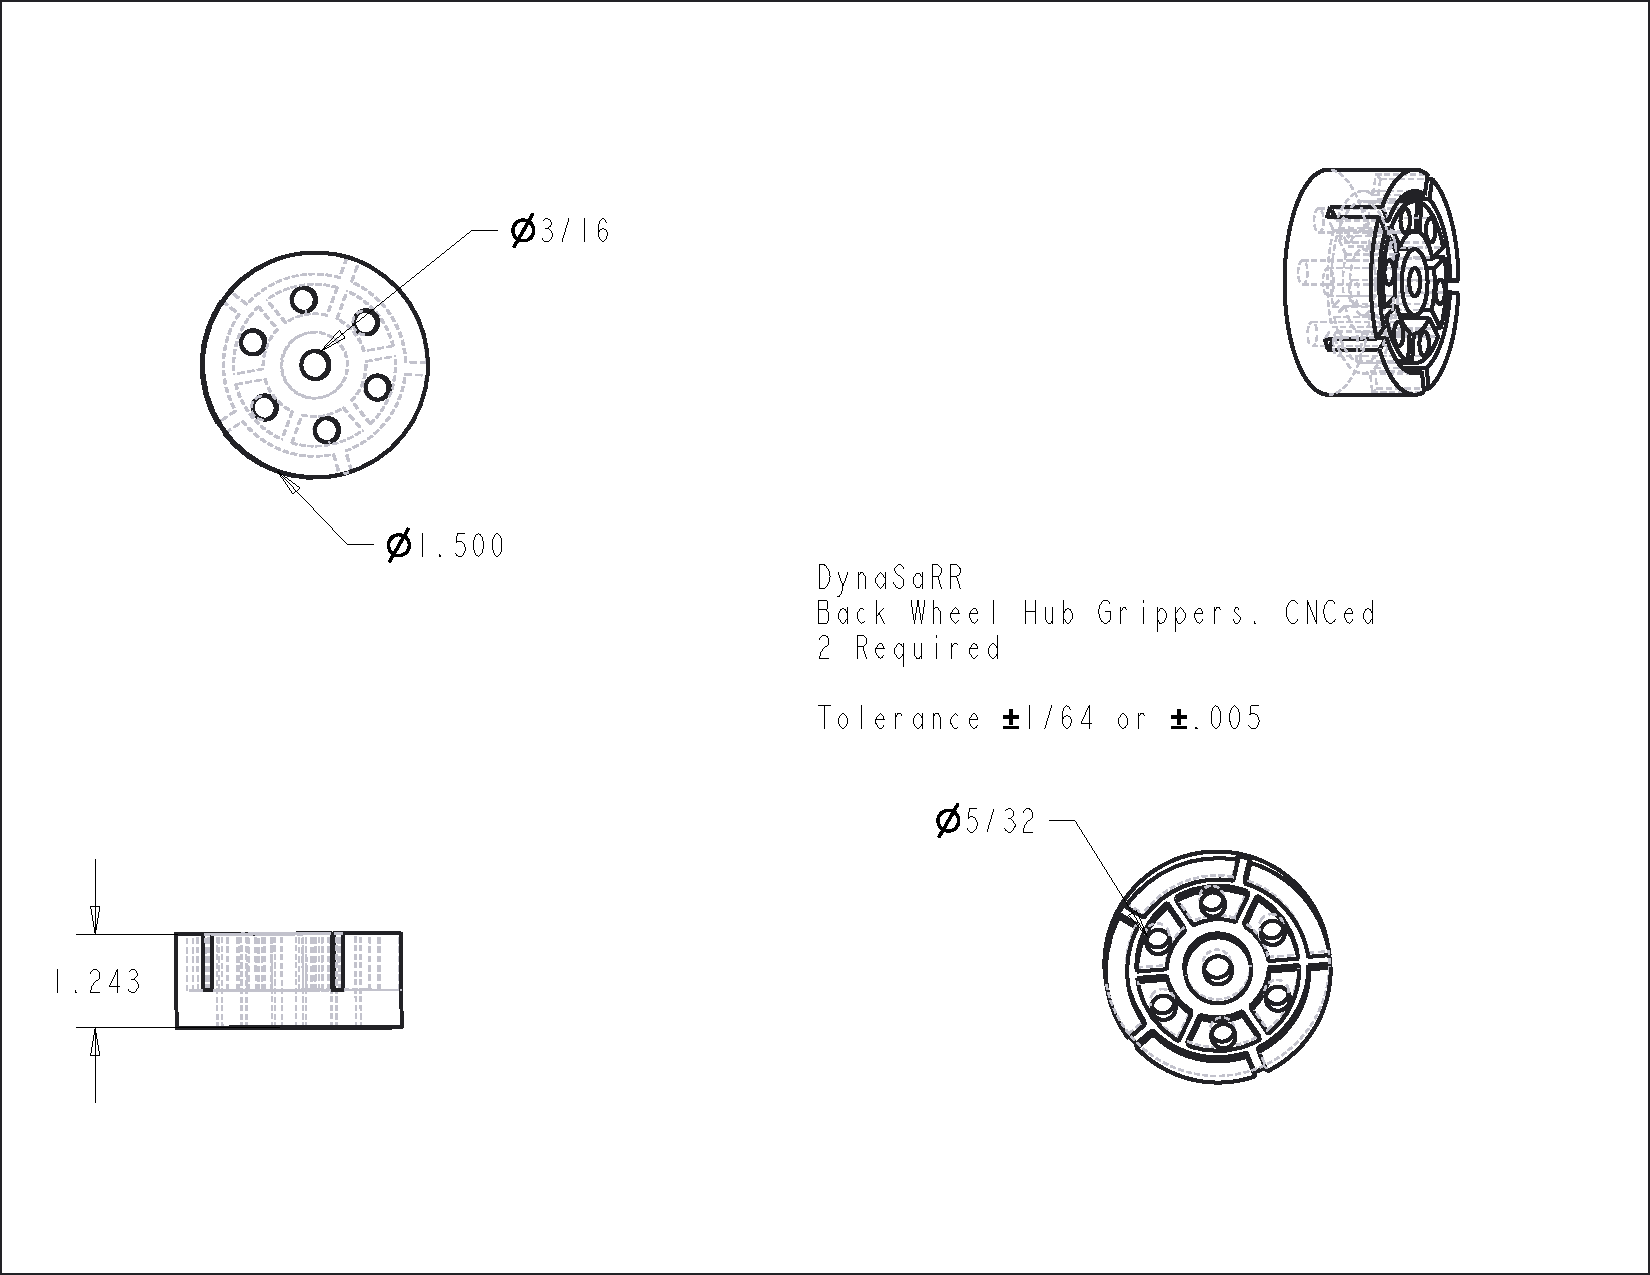
\includepdf[pages={-},angle=90]{./drawings/back_hub_gripper}
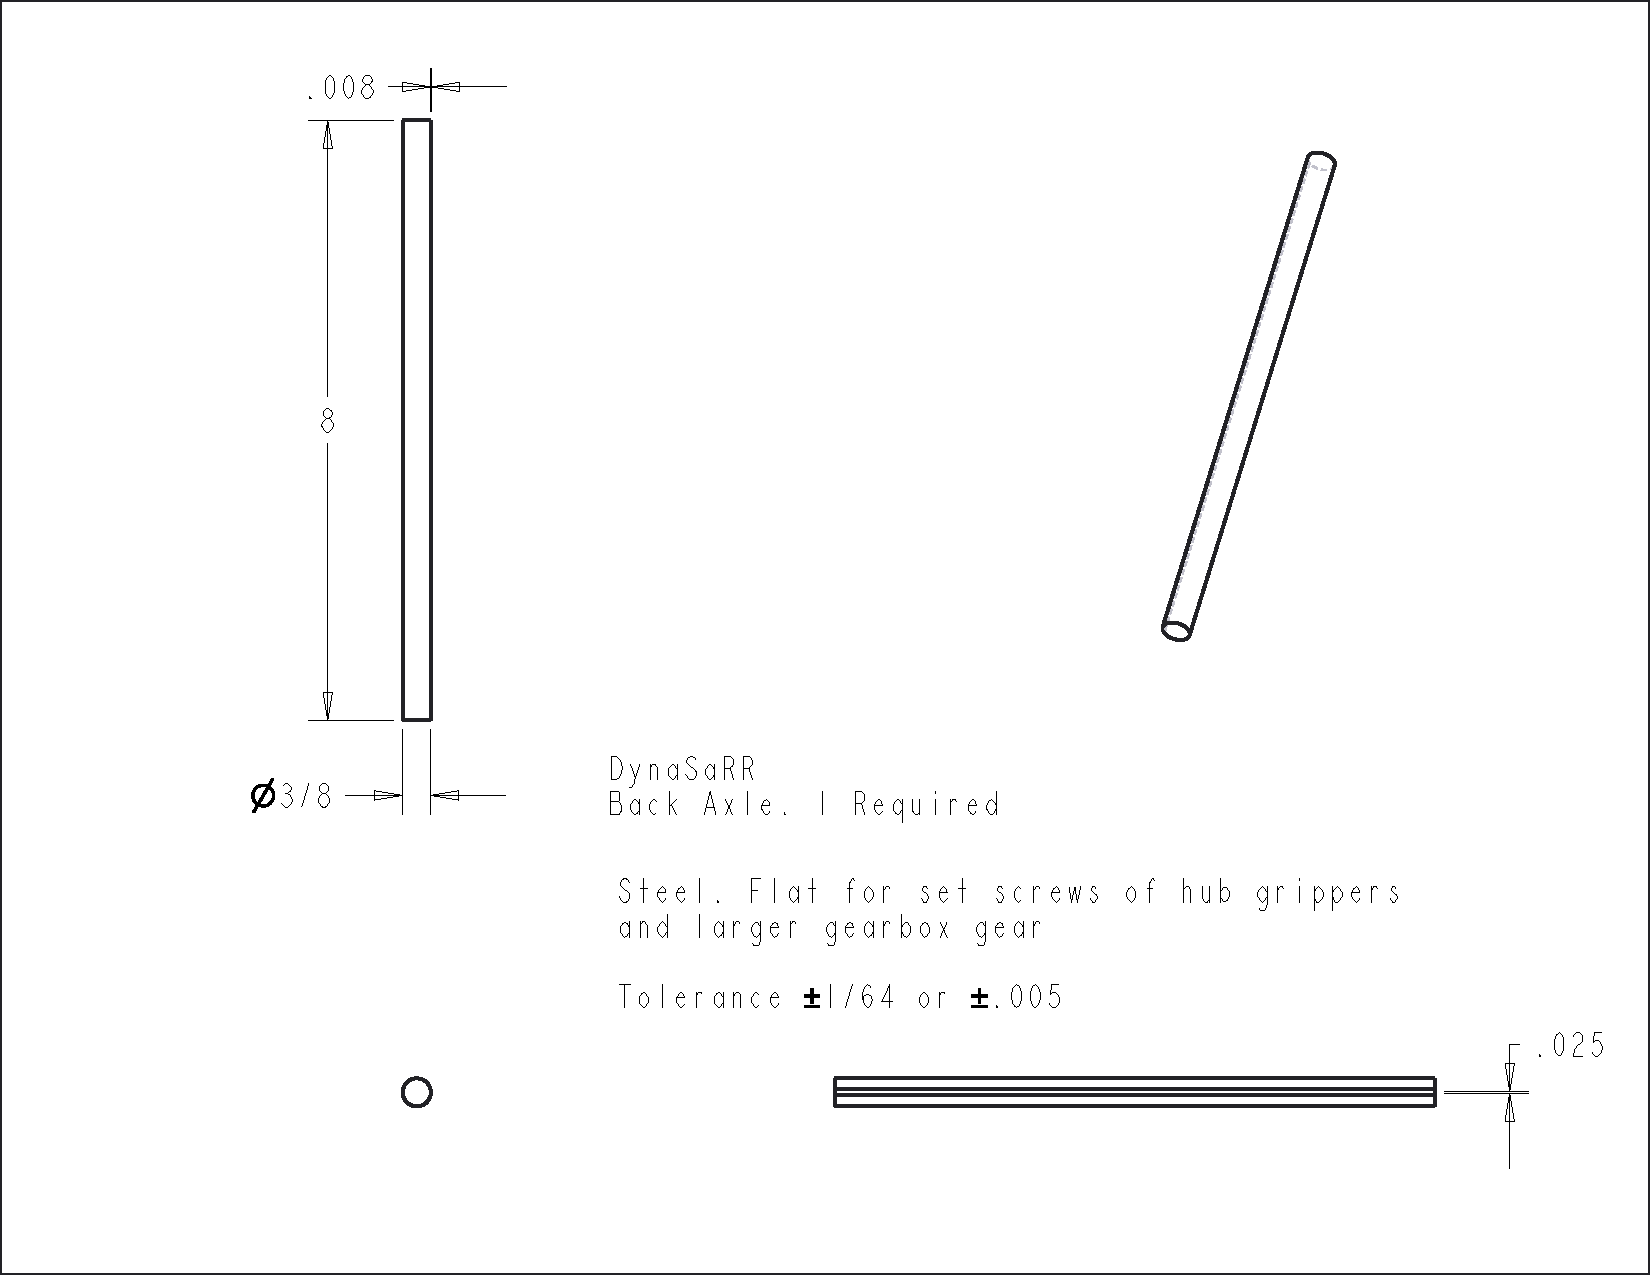
\includepdf[pages={-},angle=90]{./drawings/backaxle_drawing}
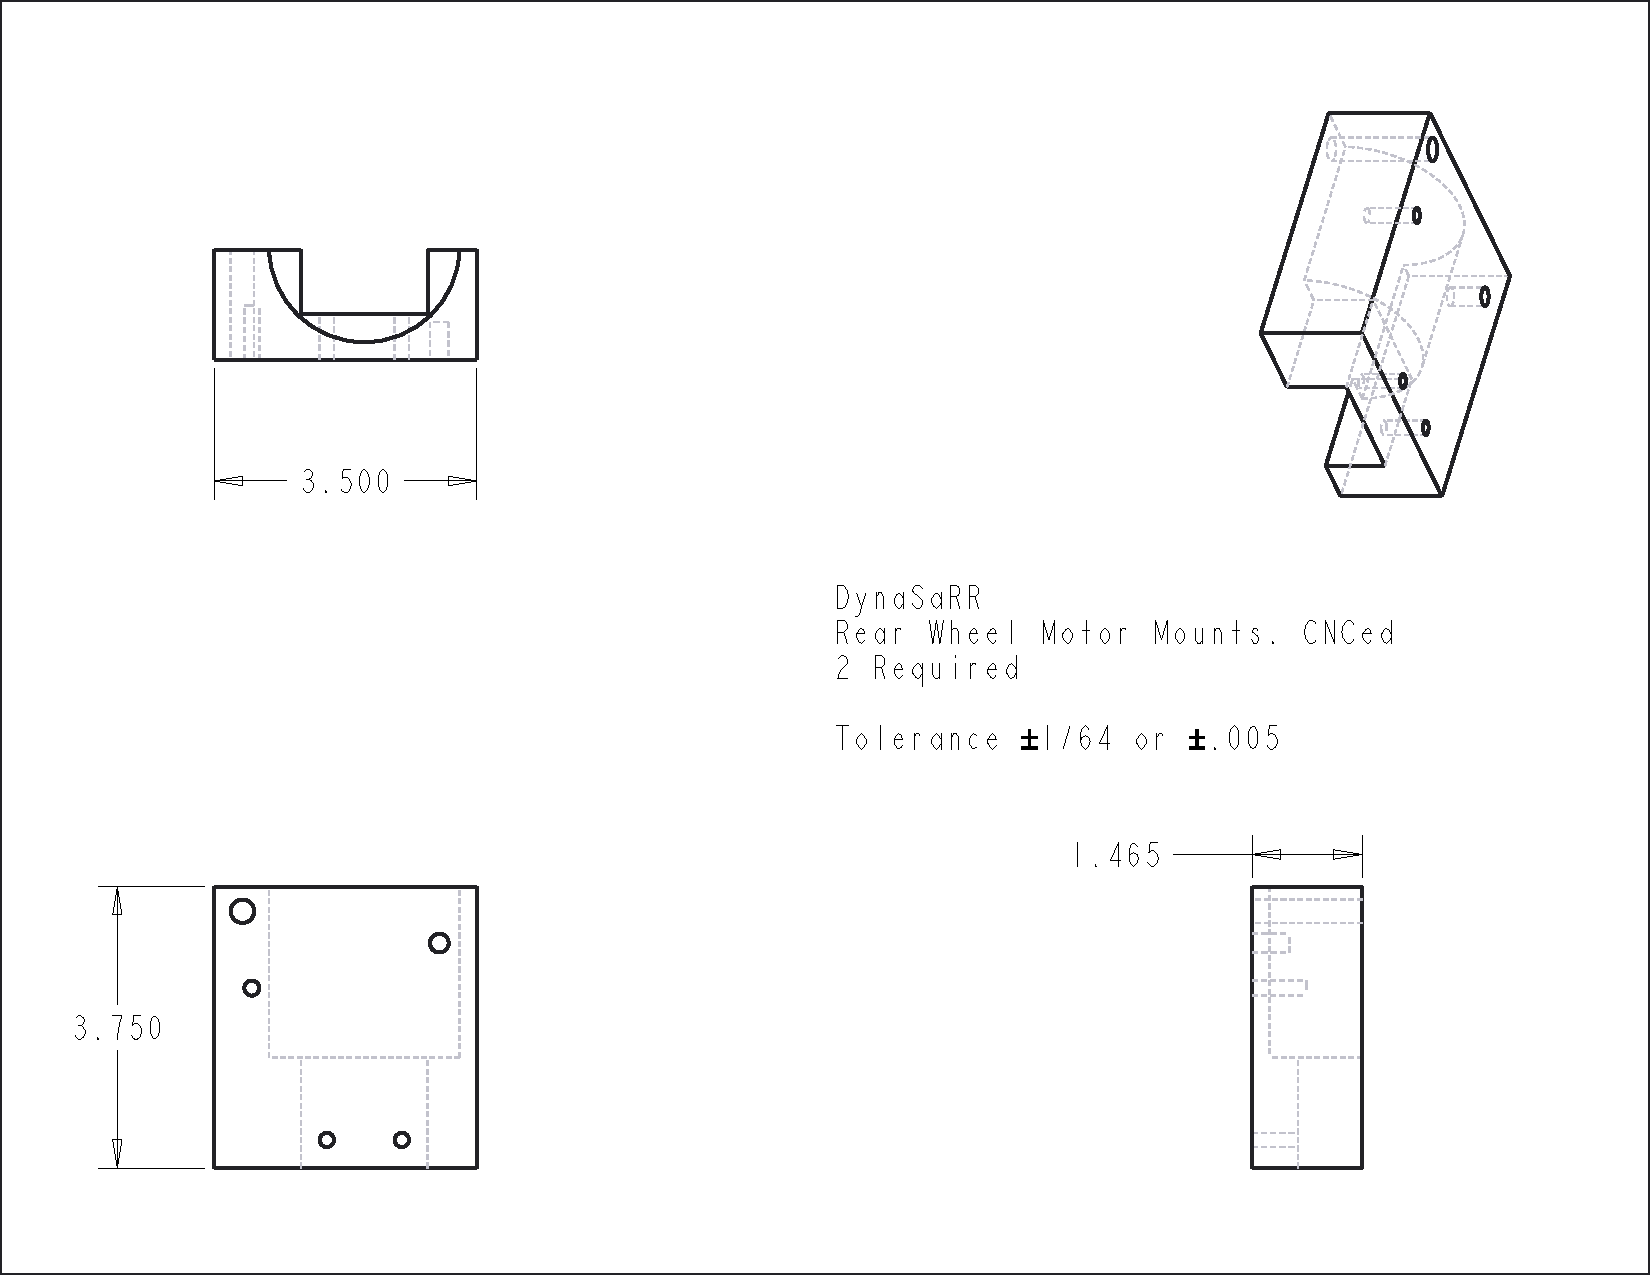
\includepdf[pages={-},angle=90]{./drawings/backwheel_motor_mount}
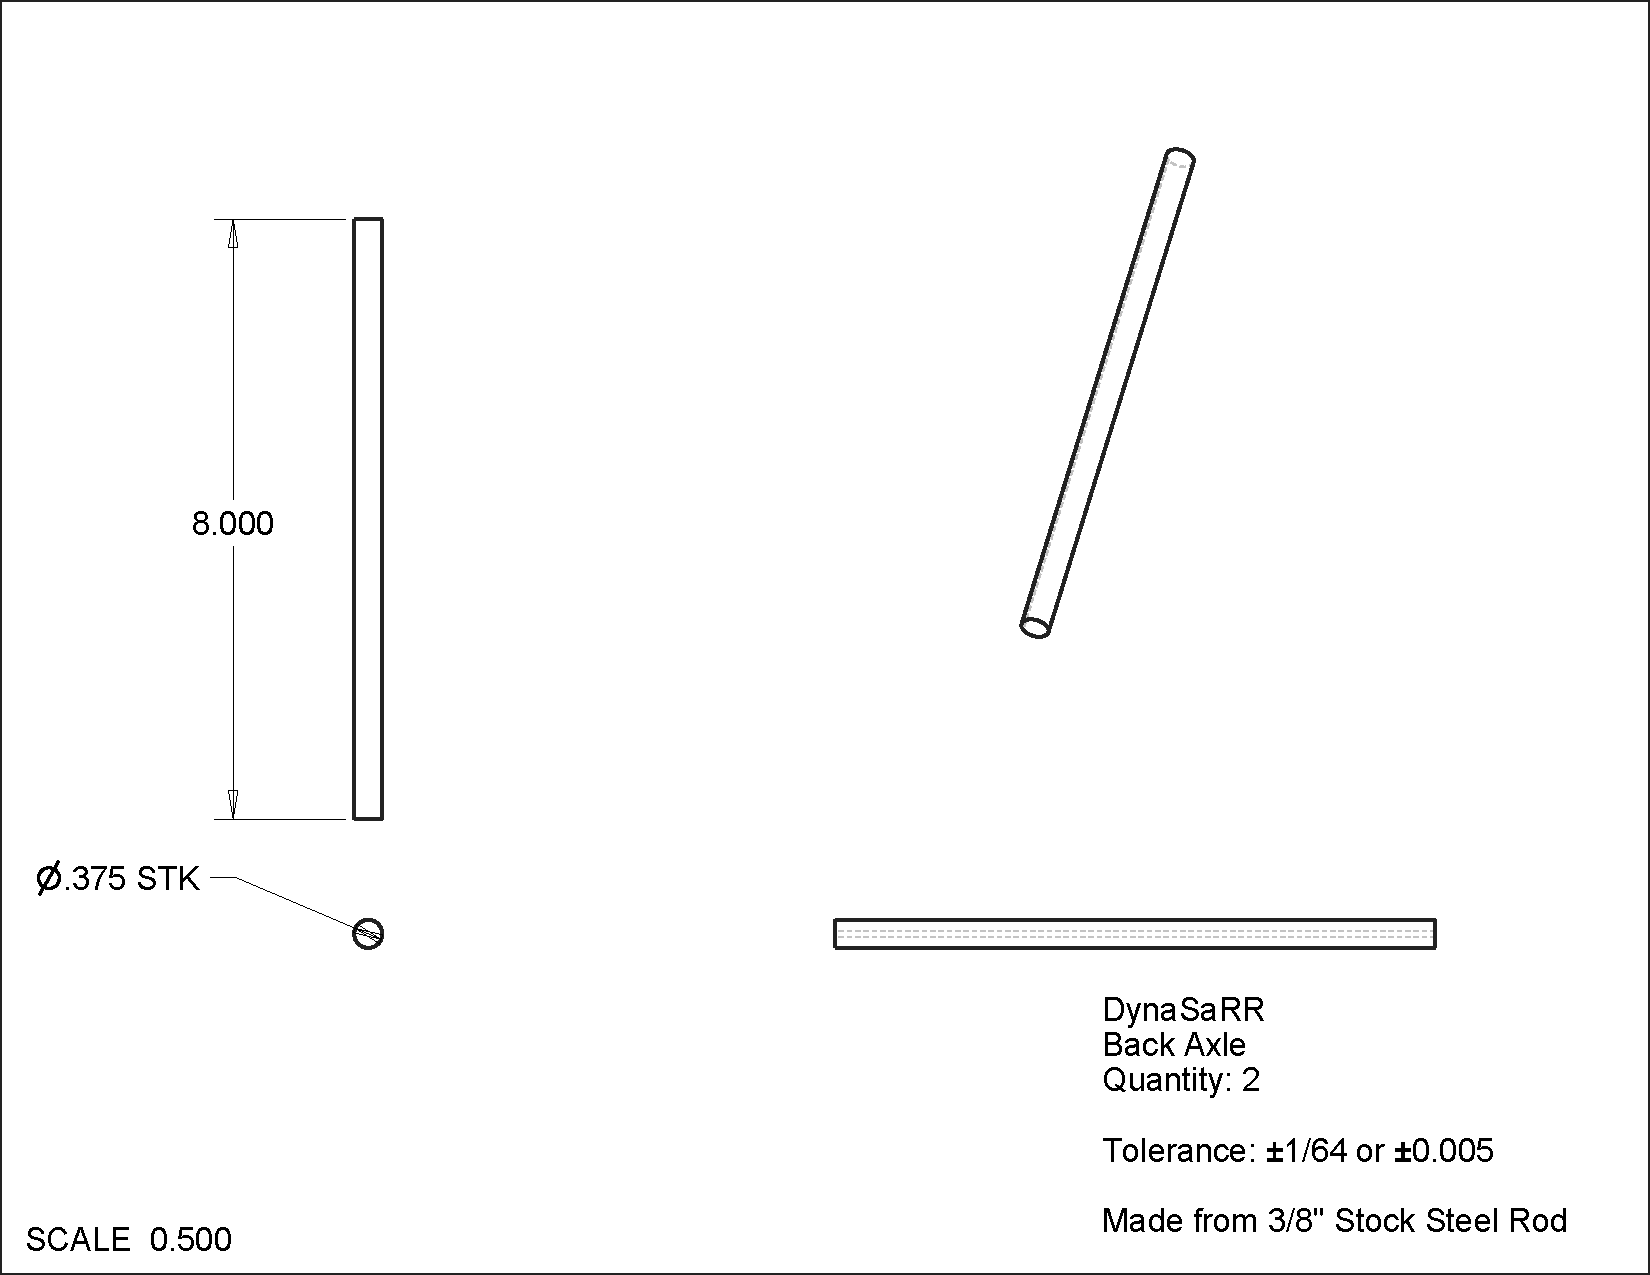
\includepdf[pages={-},angle=90]{./drawings/baxle}
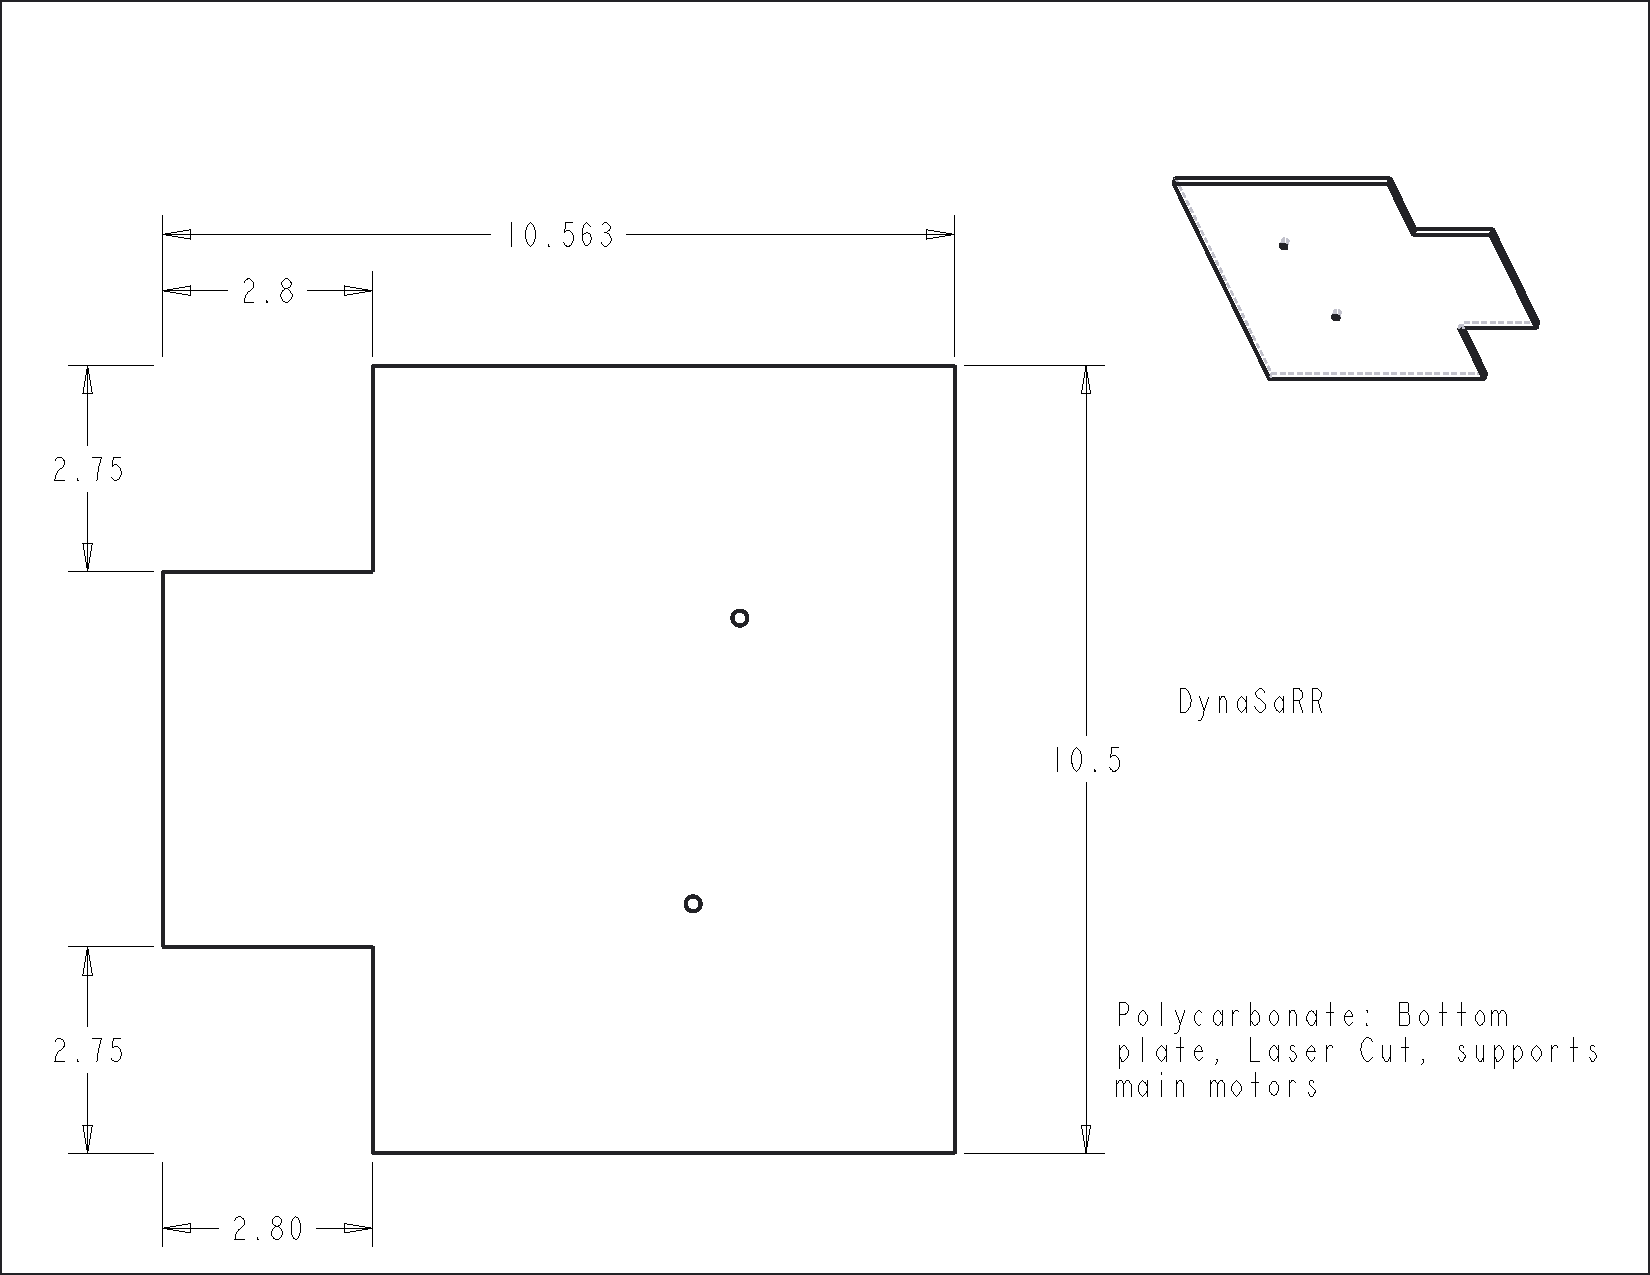
\includepdf[pages={-},angle=90]{./drawings/bottom_poly_cnc}
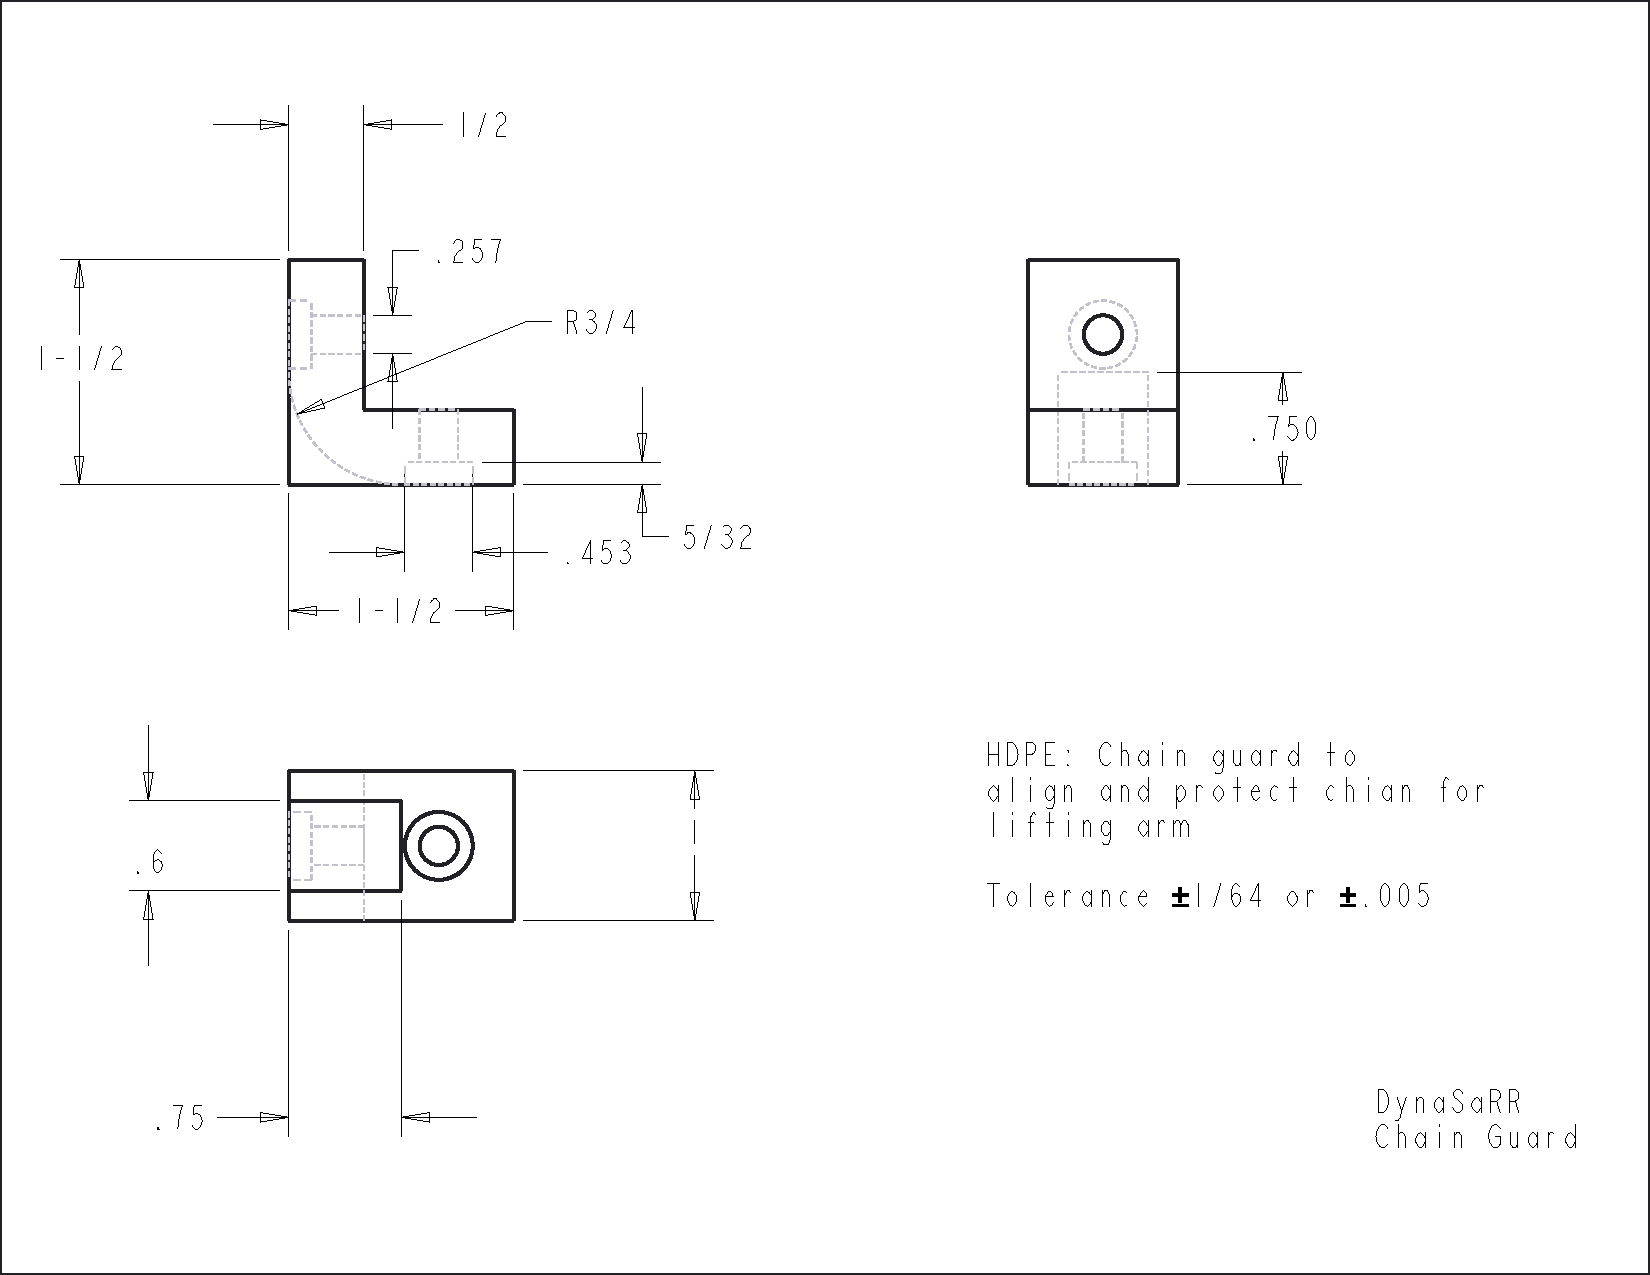
\includepdf[pages={-},angle=90]{./drawings/chain_guard}
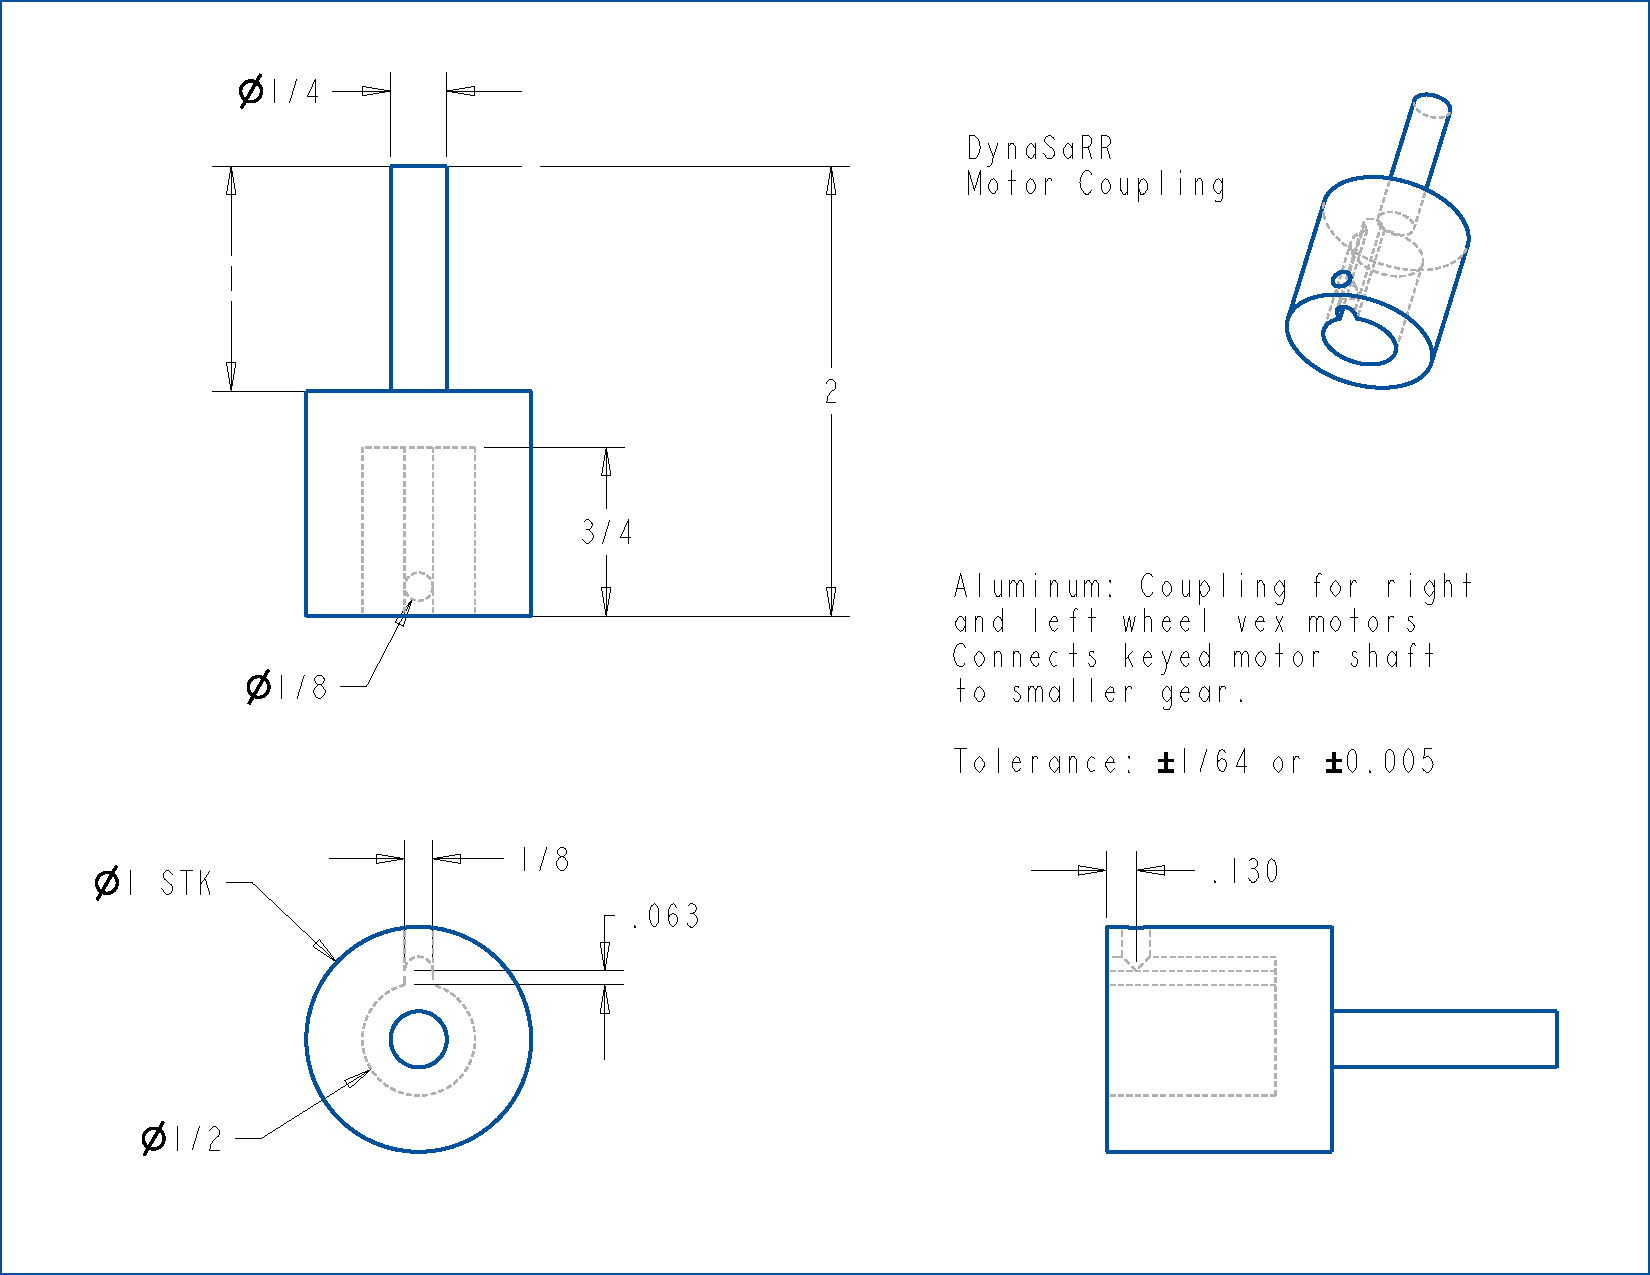
\includepdf[pages={-},angle=90]{./drawings/coupling_drawing}
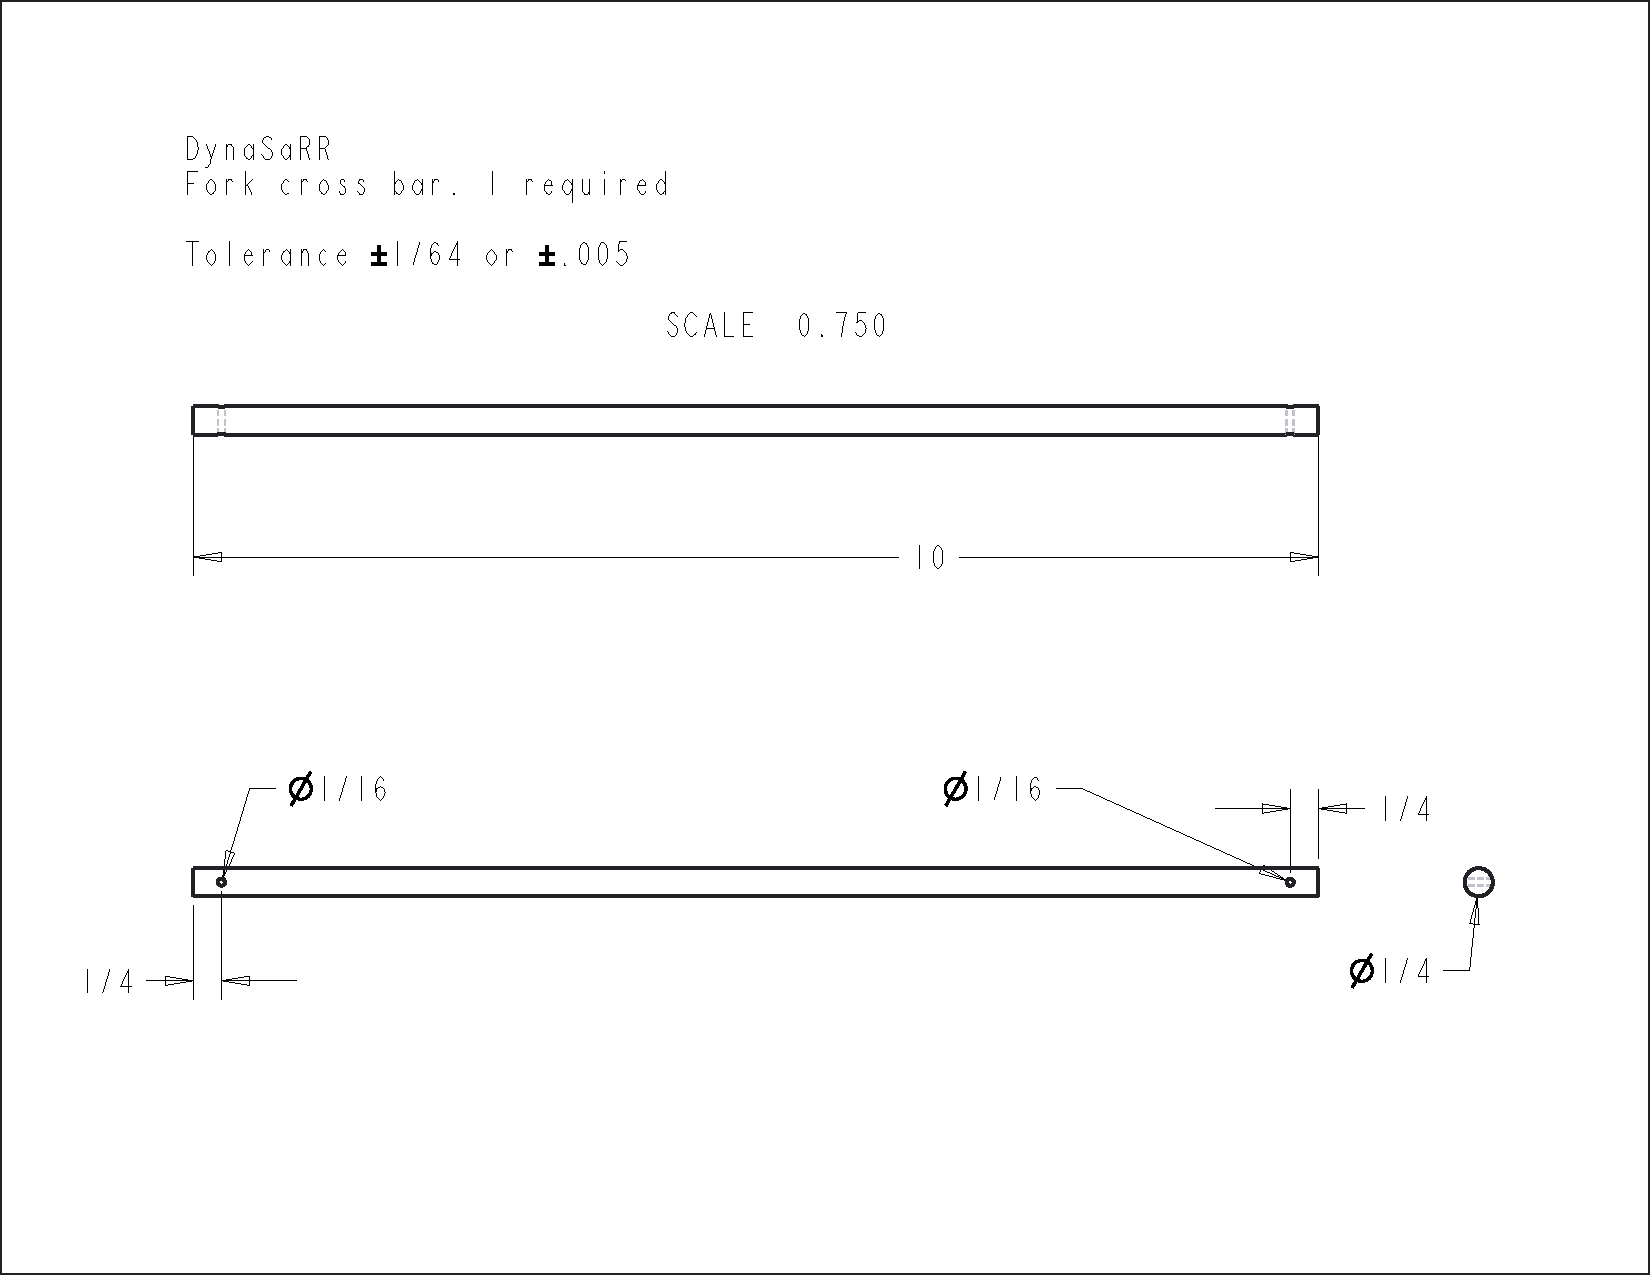
\includepdf[pages={-},angle=90]{./drawings/cross_bar}
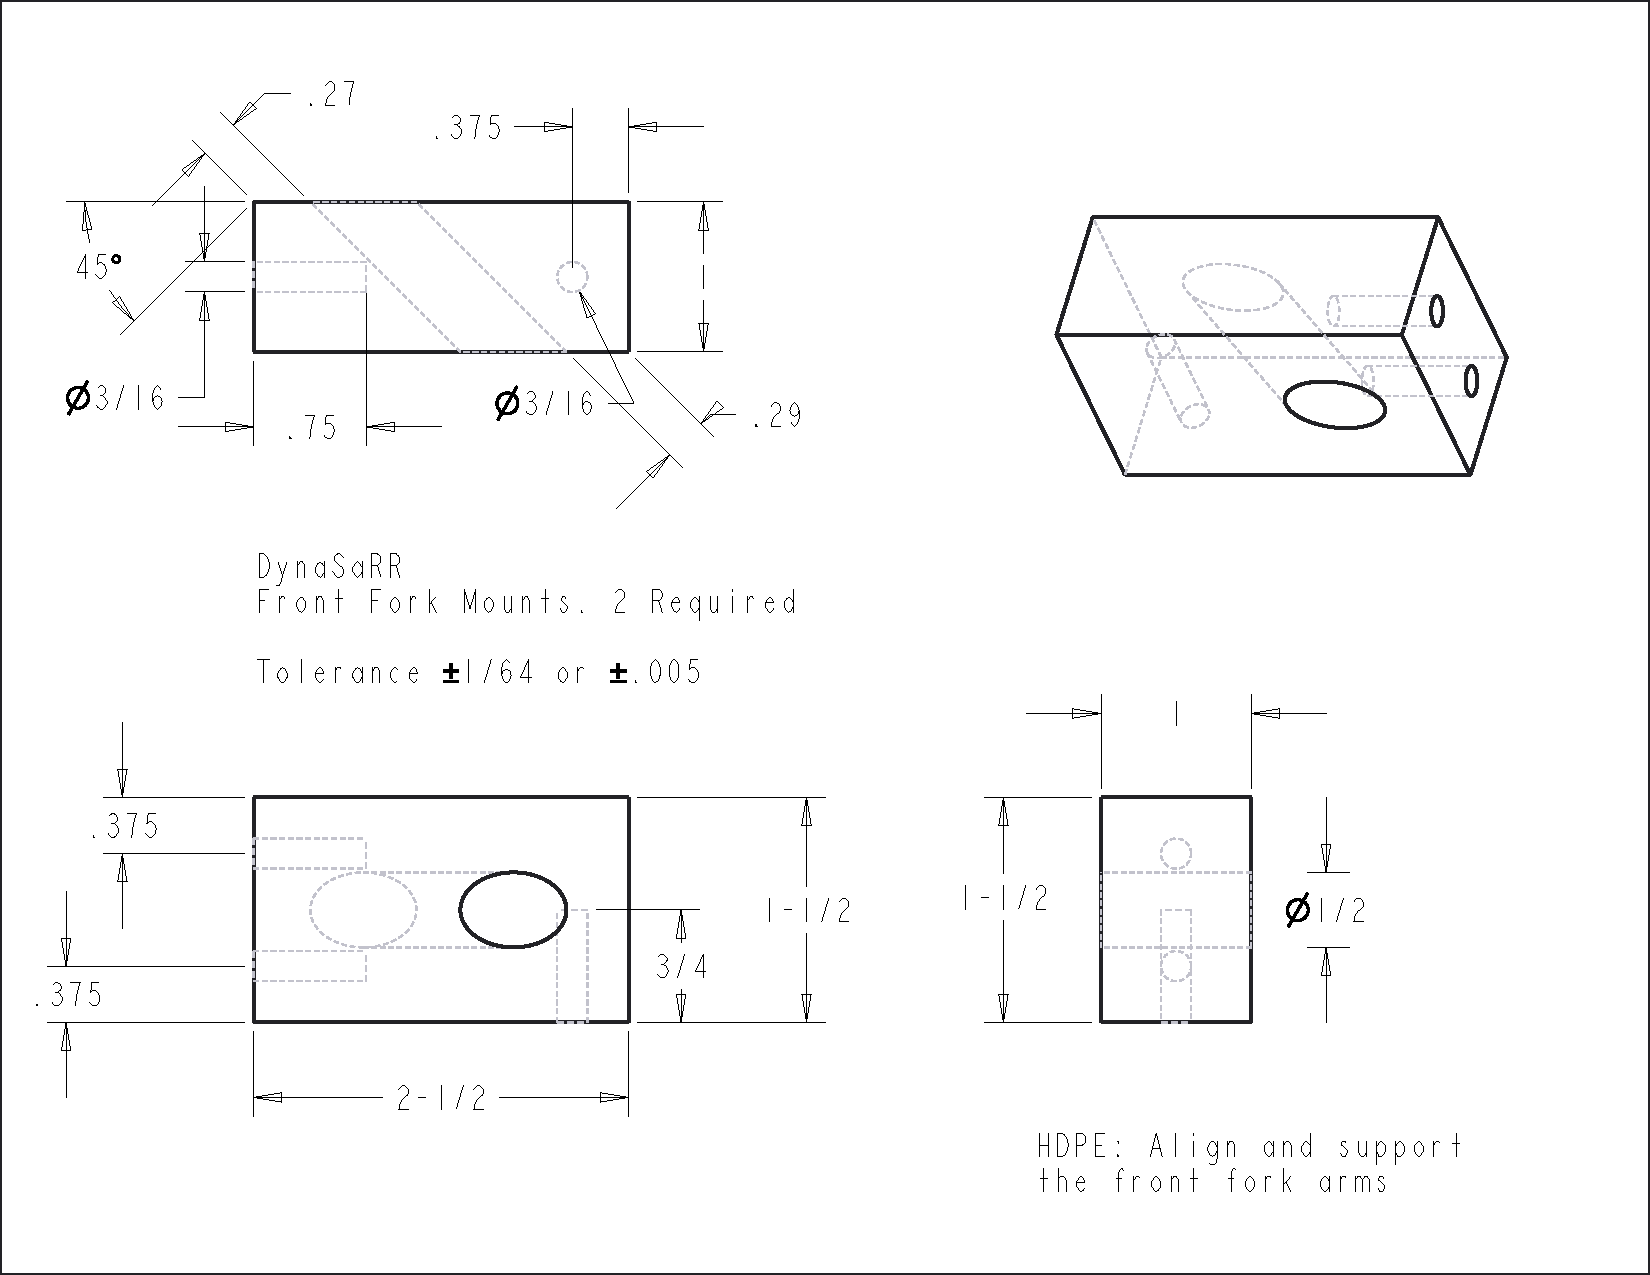
\includepdf[pages={-},angle=90]{./drawings/fork_mount_v3_left_drawing}
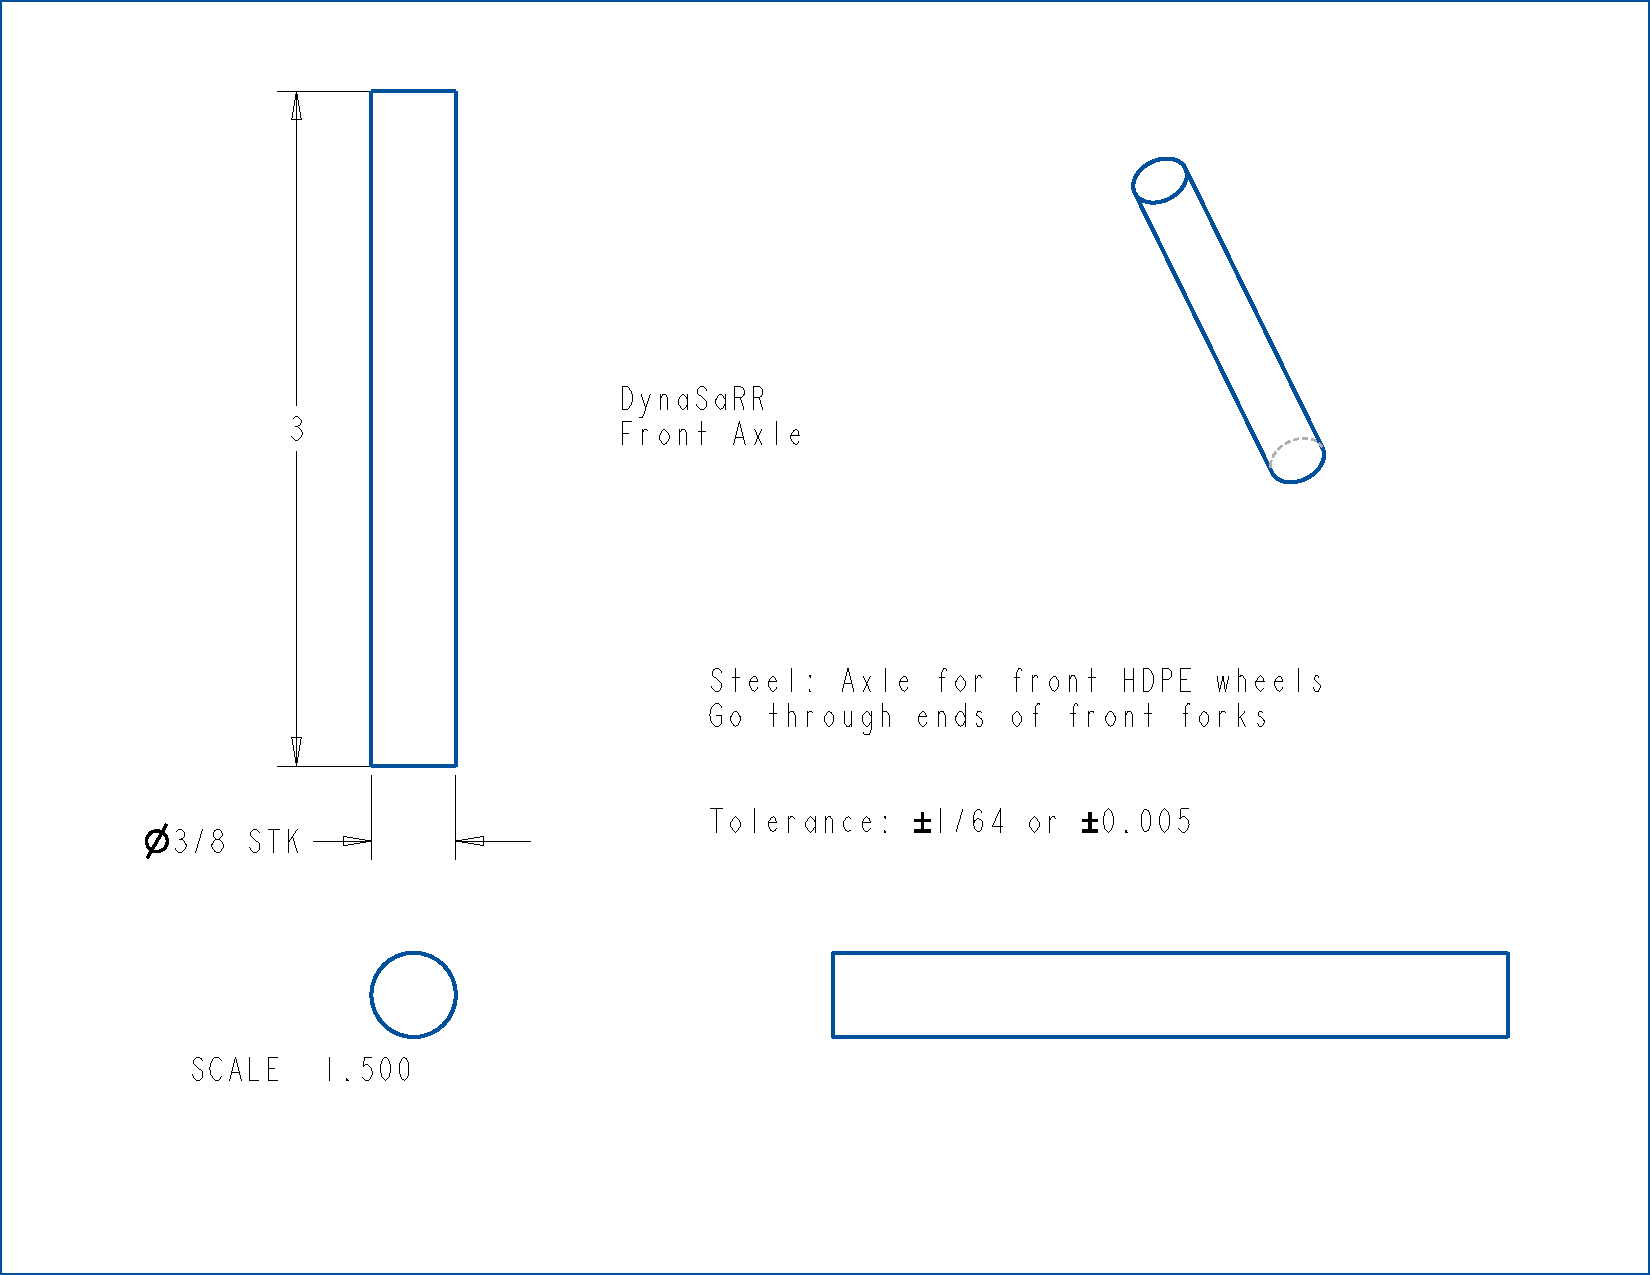
\includepdf[pages={-},angle=90]{./drawings/front_axle_drawing}
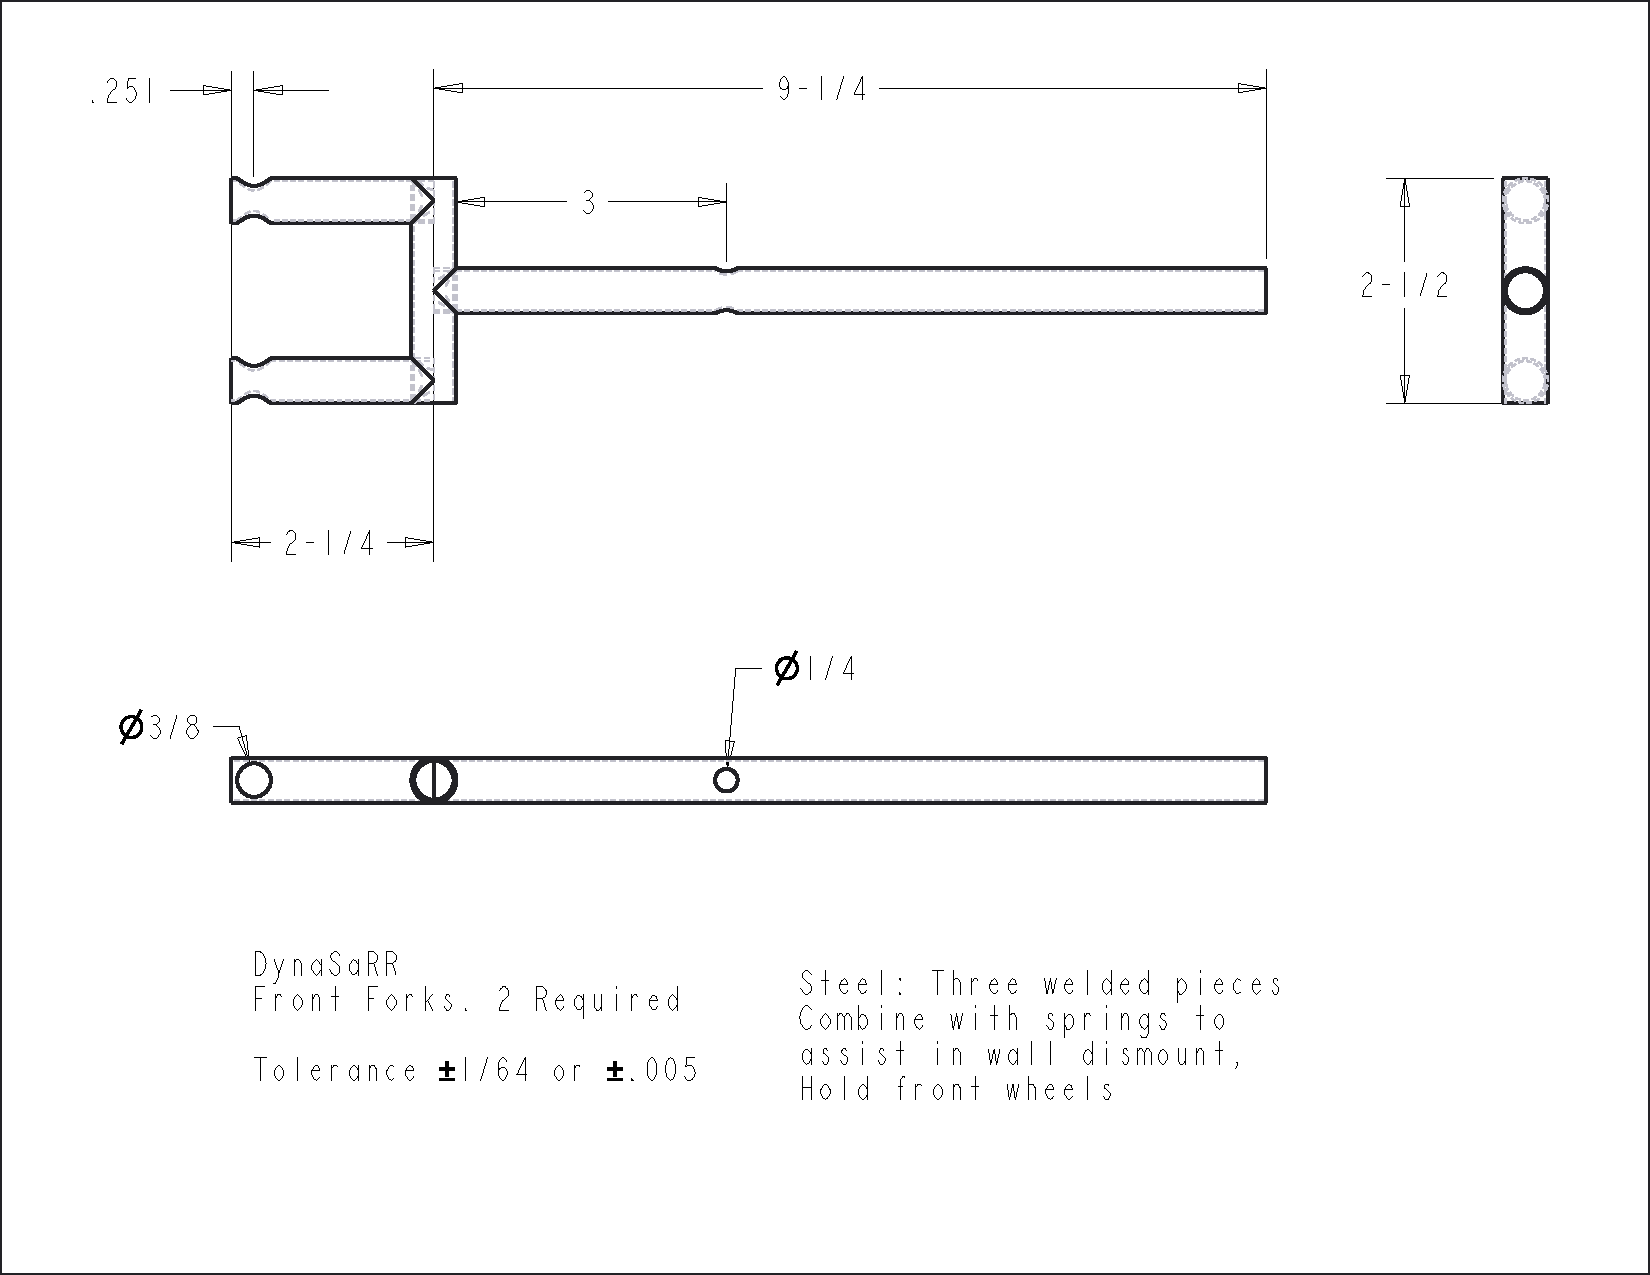
\includepdf[pages={-},angle=90]{./drawings/front_fork}
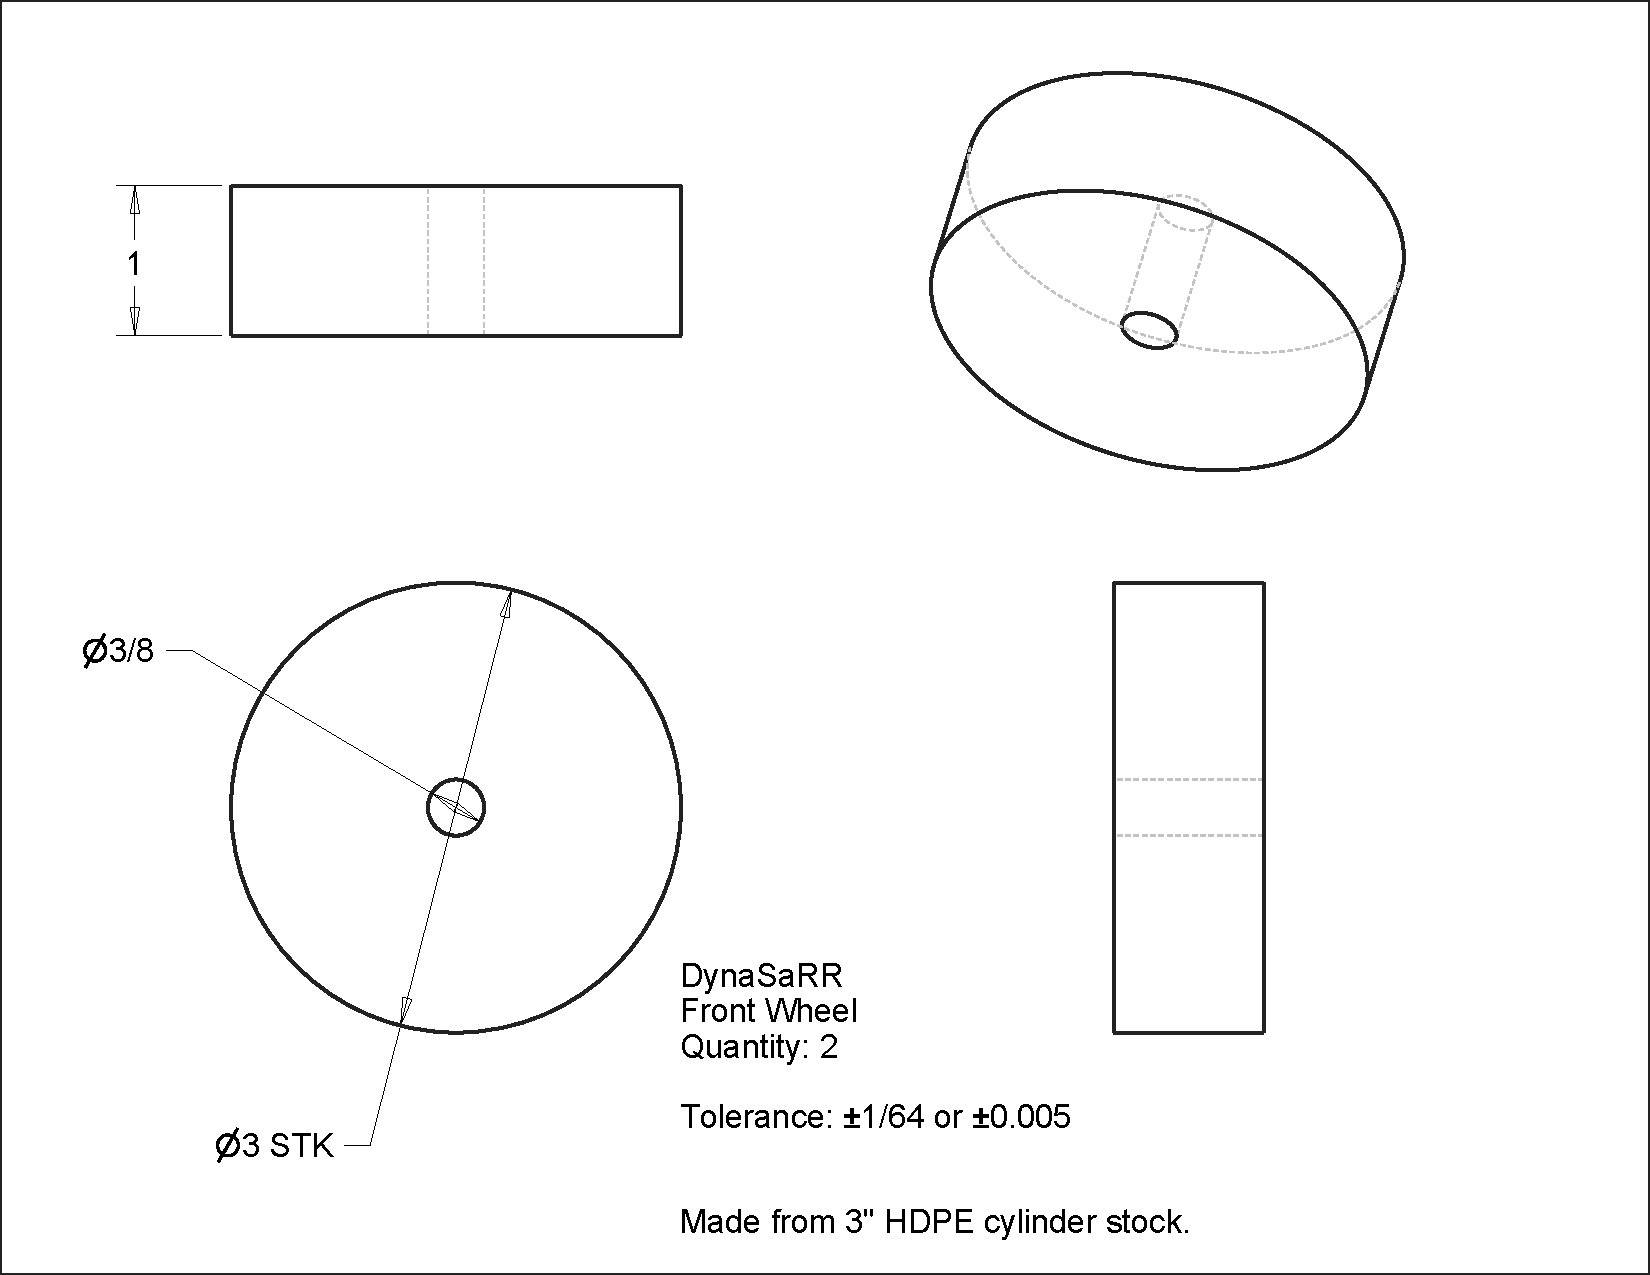
\includepdf[pages={-},angle=90]{./drawings/front_wheel_drawing}
\includepdf[pages={-},angle=90]{./drawings/gear_box}
\includepdf[pages={-},angle=90]{./drawings/gearbox_support}
\includepdf[pages={-},angle=90]{./drawings/grabber_drawing}
\includepdf[pages={-},angle=90]{./drawings/half-t-slot-v2}
\includepdf[pages={-},angle=90]{./drawings/hub_gripper_rear_drawing}
\includepdf[pages={-},angle=90]{./drawings/lifting_arm_axle_drawing}
\includepdf[pages={-},angle=90]{./drawings/lifting_arm_drawing}
\includepdf[pages={-},angle=90]{./drawings/lifting_arm_metal_gripper}
\includepdf[pages={-},angle=90]{./drawings/Lifting_Arm_Motor_Support_Cross}
\includepdf[pages={-},angle=90]{./drawings/lifting_arm_mount}
\includepdf[pages={-},angle=90]{./drawings/lifting_arm_support_cross}
\includepdf[pages={-},angle=90]{./drawings/lifting_arm_washer_plate}
\includepdf[pages={-},angle=90]{./drawings/lifting_motor_mount}
\includepdf[pages={-},angle=90]{./drawings/}
\includepdf[pages={-},angle=90]{./drawings/light-sensor_tap}
\includepdf[pages={-},angle=90]{./drawings/medkit_arm_gear_spacer_drawing}
\includepdf[pages={-},angle=90]{./drawings/medkit_axle_drawing}
\includepdf[pages={-},angle=90]{./drawings/medkit_grabber_attchmnt_drawing}
\includepdf[pages={-},angle=90]{./drawings/medkit_limit_switch_holder_frnt}
\includepdf[pages={-},angle=90]{./drawings/medkit_limit_switch_holder_rear}
\includepdf[pages={-},angle=90]{./drawings/medkit_motor_mount_bottom}
\includepdf[pages={-},angle=90]{./drawings/medkit_motor_mount_top}
\includepdf[pages={-},angle=90]{./drawings/medkit_secure_l_beam}
\includepdf[pages={-},angle=90]{./drawings/medkit_washer_plate_drawing_bottom}
\includepdf[pages={-},angle=90]{./drawings/top_cross_bar}
\includepdf[pages={-},angle=90]{./drawings/washer-plate-drawing.pdf}

\end{landscape}

\end{document}